\clearpage
\section{A pathwise volatility modelling framework}\label{chap:framework}

We are now ready to employ the new ODE theory from the previous two chapters to build a \emph{probabilistic} volatility modelling framework. We use `pathwise' (which may be considered an antonym of `probabilistic') to describe this framework as a reminder that all models within it, which will exist on some probability space $(\Omega,\cF,\PP)$, are well-defined on an explicit subset $\Omega_*\subseteq\Omega$ of outcomes (or `paths') with full $\PP$-measure. Proof of this will just follow from our probability-free well-posedness theory applied to each outcome $\omega\in\Omega_*$. This situation is more helpful than a model just being a.s.~well-defined, since this need not \emph{explicitly} provide $\Omega_*$. We do not consider there to be a standardised meaning of `pathwise' in general; see e.g.~\cite{vovk_2016} for a short background on its varied use in the context of It\^o-type integrals.

Equipped with $\Omega_*$ where $\PP[\Omega_*]=1$, our models thus remain a.s.~well-defined under any other measure $\PP_*$ verifying $\PP_*[\Omega_*]=1$, so by definition under any $\PP_*\!\ll\!\PP$. Practically, this enables us to e.g.~\emph{replace} Brownian motion in the Heston model's representation from \autoref{eq:tce} with a vast range of other (irregular) stochastic processes, \emph{with no additional well-posedness analysis required}. This is discussed following \autoref{thm:solutionmap_rand} and made precise within \autoref{def:gen_heston_frame}, where alternative volatility drivers $Z$ are defined. We make use of these when defining the RLH model in \autoref{sec:RLH_model}, where one of the Gaussian processes from \autoref{cor:gauss_heston_mgf} is used. Recall that this ability to replace Brownian motion is one of the motivations behind the pathwise theory of \cite{friz_2010} and \cite{friz_2014}.

We can only consider e.g.~the Heston SDEs from \autoref{eq:heston_intro} in an similar `pathwise' sense if we invoke pathwise It\^o calculus, originating from \cite{follmer_1981}. This is an active line of research; see \cite{davis_2018}, \cite{lochowski_2018} and \cite{cont_2019} for developments, all similarly motivated by problems in finance. Our pathwise framework built from ODEs was not designed to compete with these rough path and pathwise It\^o alternatives (rather, it emerged when treating the problems outlined in the \hyperlink{prologue}{Prologue}). But a significant benefit of it compared with these is its relative simplicity, given it does not depend on the non-Riemannian integrals at the core of these alternatives.

The programme of this chapter is now outlined before our probabilistic set-up is specified.

\vspace{3mm}\textbf{From framework to model.} Building on the ODE theory from the previous two chapters, the first half of this one serves as a three-stage funnel. A very general framework for modelling price processes on a probability space $(\Omega,\cF,\PP)$ is first defined in \autoref{sec:base_frame}. As discussed in \autoref{ch:intro}, this depends on the solutions of \autoref{prob:ivp2} for each $\omega\in\Omega$. So as per \autoref{cor:surjective_map} it is built from a non-injective and surjective solution map which by \autoref{thm:wellposed} is continuous w.r.t.~uniform convergence over compacts. This general framework is then reduced to two distinct sub-frameworks in \autoref{sec:heston_frame} and \autoref{sec:martingale}, which respectively contain generalised Heston and martingale models. Finally the funnel's specific product, the RLH model, is defined in \autoref{sec:RLH_model}, which resides in the intersection of these two sub-frameworks. This was illustrated in \autoref{fig:venn}, repeated here for convenience.

\vspace{2mm}
\begin{figure}[H]
    \centering
    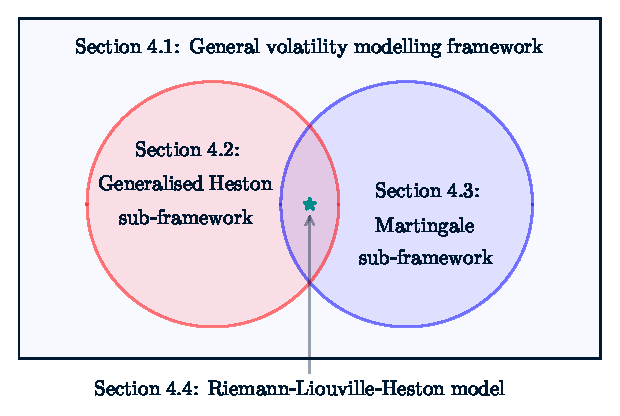
\includegraphics[width=0.60\linewidth]{figures/venn}
    \label{fig:venn2}
\end{figure}

\vspace{-6mm}

{\centering\autoref{fig:venn}: Venn diagram showing the frameworks and model defined in this chapter.\\}

\vspace{4mm}

Much care has been taken in the selection of these funnelling stages for presentation here, because we are trying to attain several goals without compromising any. Of course, we want to end up with a volatility model which exhibits some properties of the leading counterparts from other more established frameworks. But on the other hand, it is arguably more important that the route to this model is identifiable in some respect, given that the ODE-based foundations on which the framework here rests are unconventional in finance. Subject to these requirements, we must additionally show how the limiting results of \autoref{chap:solutions} can be applied to precisely characterise the Heston-NIG relationship discussed in the \hyperlink{prologue}{Prologue}. By doing this, this new framework's ability to teach us practically valuable things about others is unquestionable, not least because the Heston and NIG models are two of the most popular in finance, respectively deriving from differing (continuous and pure jump) frameworks.

This all considered, we let the Heston model take a somewhat central role throughout this chapter. Specifically, the sub-framework in \autoref{sec:heston_frame} produces a price process which is equal in distribution to the Heston model's when a process $Z$ which drives volatility is Brownian motion, but allows for this process to be replaced by essentially any other random element of $\uC_0(\RR_+,\RR)$. (A reader comfortable with stochastic processes existing only up to a non-zero but random explosion time, see e.g.~Definition 2.1 in \cite{ikeda_1989}, can omit `essentially' here.) This ability to simply replace Brownian motion cannot be taken for granted, and as just discussed is reminiscent of rough path theory advertisements.

The RLH model, the focus of \autoref{sec:RLH_model}, then constitutes the special case within this generalised Heston sub-framework where the volatility-driving Brownian motion is replaced by its Riemann-Liouville fractional derivative of some order in $(0,\frac12)$. As a result, the price process from this model coincides (in distribution) with that from the Heston model when (and only when) this derivative order is zero. Because the Riemann-Liouville fractional derivative map defines a continuous isomorphism between H\"older spaces, see e.g.~\cite{samko_1993}, it is straightforward to reconcile this RLH model with the growing evidence that volatility typically exhibits H\"older regularities much lower than that of Brownian motion.

\vspace{3mm}\textbf{Specific application choices.} The second half of this chapter focuses on applications, the last of which are the limits already mentioned, covered in \autoref{sec:price_limits}. These limits are treated in the specific case of the RLH model for maximum clarity, given the probability-free theory for any other model is provided in \autoref{chap:solutions}. As should be clear after \autoref{ex:heston_to_NIG} and  \autoref{fig:hausdorff_composite}, these limits are not just mathematical curiosities, but will provide precise answers to the questions in the \hyperlink{prologue}{Prologue}, regarding the popular Heston and NIG models.

Before this we show in \autoref{sec:vol_surfaces} how derivative prices can be simulated under the RLH model. Theoretically, this depends on both the martingale theory from \autoref{sec:martingale} and the probability-free simulation convergence from \autoref{thm:wellposed}. A background to the relevance of martingales for derivative pricing is also provided in \autoref{sec:martingale}, following the very pragmatic approaches of \cite{cont_2003} and \cite{guyon_2013}. It is specifically \autoref{cor:RLH_martingality} which establishes the RLH price process to be a martingale, by bringing together several other results, existing and new. Towards this, \autoref{thm:mgf_existence} should be noted, clarifying how martingale prices can be related to the thickness of a volatility-driving process's marginal tails, and in the wider generalised Heston sub-framework from \autoref{sec:heston_frame}.

There are two reasons for prioritising a simulation-based approach at this stage of the framework's development. Firstly, it provides a standalone framework-wide solution for pricing derivatives (or other applications like hedging or forecasting), rather than depending on model-specific probabilistic analysis, which we leave for the future. Secondly, recent research has shown that \emph{alongside} simulation, neural networks offer an alternative approach to the problems classically treated by probabilistic analysis. See e.g.~\cite{buehler_2019} for hedging and \cite{horvath_2021} for model calibration.

To aid our simulation convergence, the variance reduction methods recommended in \cite{mccrickerd_2018} are utilised, for which we have no statistical biases to report. By reconciling simulated results with analytically-available classical Heston counterparts, we gain confidence that simulations are implemented correctly and have converged sufficiently.
Concise \texttt{python} code is also provided in the \hyperlink{appendix}{Appendix} to help others implement our models.

\vspace{3mm}\textbf{Probabilistic set-up.} Given the probability-free foundations in the previous two chapters, much of this chapter could also be presented without reference to a probability measure. However, most practical applications, like ours depending on the martingales in \autoref{sec:martingale}, or the weak convergence results in both \autoref{sec:vol_surfaces} and \autoref{sec:price_limits}, are inseparable from probability. It is thus clearer to start introducing the probabilistic necessities immediately.

To this end, we will always work generally on a probability space $(\Omega,\cF,\PP)$ supporting all random elements referred to, and let $\omega$ denote an arbitrary element of $\Omega$. Often it will be possible to construct these random elements on a \emph{fixed} probability space, although for the sake of brevity we will not repeatedly do so. As an example, the RLH model from \autoref{sec:RLH_model} can be constructed on the canonical probability space supporting just a two-dimensional (2d) standard Brownian motion $W=(W^0,W^1)$ over $\RR_+$. Accordingly, we could fix $\Omega:=\uC_0(\RR_+,\RR)\times\uC_0(\RR_+,\RR)$, let $\cF:=\cB(\Omega)$ be the specific Borel $\sigma$-algebra that characterises uniform convergence over compacts, let $\PP:=\WW$ be the Wiener measure on $(\Omega,\cF)$ and let $W$ be the canonical process on $(\Omega,\cF,\PP)$, defined simply by $W(\omega):=\omega$ for each $\omega\in\Omega$. This clarifies that each outcome $\omega$ need not just be connected indirectly with a path of $W$, but it may \emph{actually be} a path of $W$. Both of the Heston and NIG processes from \autoref{eq:heston_prologue2} and \autoref{eq:nig_prologue} can be likewise constructed on this fixed space $(\Omega,\cF,\PP)$, because like all models in our framework these are built from a pathwise unique map.

We assume $(\Omega,\cF,\PP)$ supports such a 2d Brownian motion $W$, which will often be indexed by the variable $x\in\RR_+$, e.g.~$W\!=\!\{W_x\}_{x\in\RR_+}$. To do otherwise can be confusing when $W$ governs the \emph{spatial} behaviour of the random fields $Y=\{Y_{t,x}\}_{(t,x)\in\RR^2_+}$ introduced shortly, and is thereafter composed with a random IVP solution $X$, like $W^\rho_{X}$ in the Heston representation in \autoref{eq:tce2}. For consistency we will then use $\{\cF_x\}_{x\in\RR_+}$ to denote the natural filtration of $W$, and $\{\cG_t\}_{t\in\RR_+}$ for a \emph{different} filtration w.r.t.~which our price processes are martingales.

\subsection{A general price process framework}\label{sec:base_frame}

Loosely, we now want to define random counterparts $X$ of the IVP solutions $\vp$ to \autoref{prob:ivp2}. Recall from \autoref{thm:solutionset} that the solution set $\Phi$ of this problem is precisely the bijective paths in $\uC^1_0(\RR_+,\RR_+)$. A price process $S$ will be obtained from these paths via composition with geometric Brownian motion, specifically $S:=\exp(W^\rho_X - \frac12 X)$, so we call $X$ the cumulative variance of $S$, $X'$ instantaneous variance and $\sqrt{X'}$ volatility. As usual, $W^\rho$ is the 1d Brownian motion on $(\Omega,\cF,\PP)$ defined by $W^\rho:=\sqrt{1-\rho^2}W^0 + \rho W^1$ for some correlation $\rho\in[-1,1]$. There is no need to constrain how $X$ and $W$ are related, via $Y$, yet.

It is worth elaborating on this last point. We do not impose such constraints at this stage because the well-posedness of our framework does not require it, unlike others. For example, in order to even exist, the It\^o integral $\int_0^t\sqrt{V_s}\dd W_s^\rho$ from the Heston model in \autoref{eq:heston_intro2} requires that $V$ is adapted to the natural filtration of $W^\rho$. We manage to defer introducing corresponding constraints until \autoref{def:spatial_adapted}, only when we consider martingale prices.

A benefit of this deferral is that if we are not working under the constraints of martingales, e.g.~if our application is volatility forecasting rather than derivative pricing, then we do not have to check the condition in \autoref{def:spatial_adapted}. What we pay for this freedom is that in full generality, where $Y$ and $W$ are merely random elements on the same space $(\Omega,\cF,\PP)$, the correlation $\rho$ and process $W^\rho$ are theoretically redundant. We choose to continue using these to define our price processes, however, because in our applications we will use them consistently with their introduction in \autoref{eq:heston_intro}. Namely, we will use $\rho$ to control the correlation between a price $S$ and its volatility $\sqrt{X'}$, often referred to as a leverage effect in equity markets. This effect may be detected in the at-the-money implied volatility skews in \autoref{fig:heston_comparison_skewed}, defined in \autoref{eq:skew_curv}, and also in the paths of $S$ and $V:=X'$ in \autoref{fig:simulation_output}.

\vspace*{2mm}
A question now arising from this loose description is: in what sense should $X$ (and $S$) be considered a bona fide stochastic process, e.g.~into which function topology does $X$ actually define a measurable map from $(\Omega,\cF,\PP)$? Recall from \autoref{thm:wellposed} that the solution map of \autoref{prob:ivp2} is continuous between $\uG\subset\uC(\RR_+^2,\RR)$ and $\uC(\RR_+,\RR)$ w.r.t.~the norms $\Vert\cdot\Vert_{\RR_+^d}$ which characterise uniform convergence over compacts. So this solution map is clearly measurable between the induced $\sigma$-algebras (topologies). So provided the random counterparts of the functions $g\in\uG$ in \autoref{prob:ivp2} are measurable from $(\Omega,\cF,\PP)$, then $X$ (and $S$) will also be. This random counterpart of $g\in\uG$ is called a random field, introduced in \autoref{def:rand_field}.

We only invoke \autoref{thm:wellposed} above because we can, and the measurability of $X$ and $S$ can be established directly. For this a sequence of (measurable) forward Euler polygon processes with vanishing mesh can be utilised, the convergence of which is ensured by \autoref{thm:euler_converge}. This approach mirrors that in Section 2.1.2 of \cite{han_2017}, where Picard-Lindel\"of sequences are used because the counterparts to our functions $g\in\uG$ are spatially Lipschitz.

\vspace{3mm}\textbf{Random fields and IVPs.} In this part the random counterpart to \autoref{prob:ivp2} is stated, for which we introduce continuous random fields. In our setting, these will be random elements of $\uC(\RR_+^2,\RR)$, but the meaning from other domains will be clear. We utilise the notation $Y=\{Y_{t,x}\}_{(t,x)\in\RR_+^2}$ from \cite{barndorff-nielsen_2018} to denote these, despite the application there being to `ambit stochastics'. Now recall the norm $\Vert\cdot\Vert_{\RR_+^2}$ on $\uC(\RR_+^2,\RR)$ used in \autoref{thm:wellposed}, which induces the topology of uniform convergence over compacts.

\begin{definition}[Continuous random field]\label{def:rand_field}
    Let a continuous random field $Y=\{Y_{t,x}\}_{(t,x)\in\RR_+^2}$ be any random element of $\uC(\RR_+^2,\RR)$. That is, any measurable map from $(\Omega,\cF,\PP)$ to the set $\uC(\RR_+^2,\RR)$ equipped with the Borel $\sigma$-algebra induced by the norm $\Vert\cdot\Vert_{\RR_+^2}$ on $\uC(\RR_+^2,\RR)$.
\end{definition}

Using continuous random fields (hereafter just random field), random ODEs and IVPs, and their solutions, can be defined as a natural extension of their non-random counterparts. We define solutions over all of $\RR_+$ because we are most interested in IVPs like \autoref{prob:ivp2} where maximal solutions are global. Reducing this to compact subsets of $\RR_+$ is straightforward.

\begin{definition}[Random IVP]\label{def:rand_ivp}
    For a random field $Y=\{Y_{t,x}\}_{(t,x)\in\RR_+^2}$ on $(\Omega,\cF,\PP)$, call a stochastic process $X=\{X_t\}_{t\in\RR_+}$ a solution of the random ODE `$x'=Y_{t,x}$' if $X$ a.s.~verifies $X'_t = Y_{t,X_t}$ over $\RR_+$. Call $X$ a solution of the random IVP `$x'=Y_{t,x}$, $x_0=0$' if also $X_0=0$.
\end{definition}

As noted in \autoref{ch:intro}, our definition is consistent with the `SP' (sample path) formulation of random ODEs in \cite{strand_1970}, which is based on the author's PhD thesis \cite{strand_1968}. This should be contrasted with the definition given e.g.~in \cite{han_2017}, which is consistent with those from \cite{soong_1973} and \cite{sussmann_1978}, all extending the definition from \cite{srinivasan_1971}. Specifically, fixing a stochastic process $Z=\{Z_t\}_{t\in\RR_+}$ and function $h\in\uC(\RR^2,\RR)$, then \cite{han_2017} would ask that a random ODE solution $X=\{X_t\}_{t\in\RR_+}$ verifies an expression like $x'=h(Z_t,x)$ over $\RR_+$, i.e.~$X'_t=h(Z_t,X_t)$.

We discussed briefly in \autoref{ch:intro} why this is too restrictive for volatility modelling, because even in the Heston case of \autoref{eq:tce2} we instead have $x'=h(t,Z_x)$, so $X'_t=h(t,Z_{X_t})$. Classical random ODE theory avoids such cases for good reason, because most desirable (random) functions of type $h(t,Z_\cdot)$ violate the Lipschitz condition which is relied upon for well-posedness properties. In the Heston case, $h(t,Z_\cdot)$ inherits the regularity of Brownian motion so is only H\"older continuous of orders in $(0,\frac12)$. This kind of reasoning motivates similarly pessimistic remarks in \cite{soong_1973} regarding spatially Lipschitz random ODEs.

Following \autoref{def:rand_ivp}, the class of problems considered in this chapter may be obvious, but worth stating clearly before clarifying their well-posedness. Recall the subset $\uG\subset\uC(\RR_+^2,\RR)$ of functions from \autoref{def:mod_driving_func}, to which most results in \autoref{chap:wellposed} and \autoref{chap:solutions} apply.

\begin{problem}\label{prob:random_ivp}
    Fix a random field $Y=\{Y_{t,x}\}_{(t,x)\in\RR^2_+}$ which is a.s.~in the set $\uG$. Then find a stochastic process $X=\{X_t\}_{t\in\RR_+}$ which solves the random IVP $x'=Y_{t,x}$, $x_0=0$ over $\RR_+$.
\end{problem}

For each outcome $\omega\in\Omega$, the (non-random) IVP $x'=Y_{t,x}(\omega), x(0)=0$ then a.s.~provides an example $x'=g_\omega(t,x), x(0)=0$ of \autoref{prob:ivp2}, given a.s.~$g_\omega(t,x)=Y_{t,x}(\omega)\in\uG$. From a probabilistic perspective, our use of `Fix\dots Then\dots' in \autoref{prob:random_ivp} should be noted. This is because we are in the privileged situation where we \emph{can} first fix $Y$ and \emph{will} be able to find a solution $X$, never having to seek the couple $(X,Y)$ simultaneously. To borrow terminology from SDEs, we are seeking only \emph{unique strong} solutions. If found for arbitrary $Y$ in $\uG$, this is `the best possible situation', as described in Figure 1.1 from \cite{cherny_2005}.

In a related vein, whenever we refer to stochastic processes like $X$, e.g.~a unique solution of \autoref{prob:random_ivp}, we are as usual referring to an equivalence class of indistinguishable stochastic processes. Only \autoref{thm:rand_well_posed} acknowledges this explicitly, by constructing one solution $X$ to \autoref{prob:random_ivp} and clarifying that any other $X^*$ is indistinguishable, i.e.~a.s.~verifies $X^*=X$.

\vspace{3mm}\textbf{Well-posedness.} By considering the random IVPs in \autoref{prob:random_ivp} driven only by random fields $Y$ a.s.~in $\uG$, we can draw upon the probability-free analysis in the previous two chapters. The next result specifically clarifies the consequences of \autoref{thm:wellposed} for \autoref{prob:random_ivp}. We will henceforth omit the repetition of `a.s.' when it is clear to do to so, e.g.~writing $Y\in\uG$. Such an assumption \emph{implies} that the set $\{\omega\in\Omega:Y(\omega)\in\uG\}$ is measurable, i.e.~in $\cF$. In turn any countable intersection of full-measure sets is measurable by the properties of $\sigma$-algebras, and retains full-measure by \autoref{eq:full_measure}. This is precisely why our probability-free theory can be applied on a pathwise basis to obtain a.s.~results, as the next proof demonstrates.
\begin{theorem}[Well-posedness for \autoref{prob:random_ivp}]\label{thm:rand_well_posed}
    All of the probability-free statements in \autoref{thm:wellposed}, applicable to a solution of \autoref{prob:ivp2}, apply on an a.s.~basis to a solution of \autoref{prob:random_ivp}, i.e.~to a solution of a random IVP $x'=Y_{t,x}$, $x_0=0$ with $Y\in\uG$. Specifically\emph{:}

    \emph{1 (Global existence and uniqueness).} There exists a unique solution $X=\{X_t\}_{t\in\RR_+}$ of any such random IVP. This solution has paths in the set $\Phi\subset\uC^1_0(\RR_+,\RR_+)$ from \autoref{def:solutionset}\emph{;}

    \emph{2 (Upper bound).} This solution $X$ is dominated by the process $\bX=\{\bX_t\}_{t\in\RR_+}$ defined by $\bX_t=\inf\{x>0:Y_{t,x}<0\}$, which has paths in the set $\bPhi\subset\uD(\RR_+,\RR_+)$ from \autoref{def:setE}\emph{;}

    \emph{3 (Continuous dependence).}$\!$ The solution map of \autoref{prob:random_ivp} is continuous from $\uG$ to $\Phi$ w.r.t.~uniform convergence over compacts. That is, if $\{Y^n\}_{n\in\NN_0}$ generate solutions $\{X^n\}_{n\in\NN_0}$,~
    \begin{equation}\label{eq:cont_dep_sim}
        \Vert Y^0-Y^n\Vert_{\RR_+^2}\xrightarrow[\mathrm{a.s.}]{n\to\infty}0\quad \implies\quad \Vert X^0- X^n\Vert_{\RR_+}\xrightarrow[\mathrm{a.s.}]{n\to\infty}0.
    \end{equation}
\end{theorem}
\begin{proof}
    Let the subset $\Omega_*\subset\Omega$ of outcomes be defined by $\Omega_*:=\{\omega\in\Omega:Y(\omega)\in\uG\}$. Given that $Y\in\uG$ by assumption, we know this set $\Omega_*$ has full measure, i.e.~$\PP[\Omega_*]=1$. For each $\omega\in\Omega_*$, the (non-random) IVP $x'=g_\omega(t,x):=Y_{t,x}(\omega)$, $x(0)=0$ constitutes an example of \autoref{prob:ivp2}, so adheres to the well-posedness results of \autoref{thm:wellposed}. In particular, for each $\omega\in\Omega_*$, this IVP has a unique solution $\vp=\vp_\omega$ which is bounded above by the path $\bvp=\bvp_\omega$. Checking $(\vp,\bvp)\in\Phi\times\bPhi$ is straightforward given \autoref{thm:wellposed} and these sets' definitions.

    Now by simply defining $X(\omega):=\vp$ and $\bX(\omega):=\bvp$ for each $\omega\in\Omega_*$, processes $X$ and $\bX$ are constructed with the claimed properties in points 1.~and 2. here. There are technically other processes $X^*$ which solve \autoref{prob:random_ivp} for this choice of field $Y$, but assuming these \emph{are not} indistinguishable from $X$ provides a subset of $\Omega_*$ with positive measure where the uniqueness statement in \autoref{thm:wellposed} is violated. So indistinguishability $X^*=X$ is ensured.

    The continuous dependence statement in \autoref{eq:cont_dep_sim} follows in a similar way by applying \autoref{thm:wellposed} on a subset $\Omega_*\subset\Omega$ of outcomes with full measure. Specifically, we can define
    \begin{equation}
        \Omega_n:=\{\omega\in\Omega: Y^n(\omega)\in\uG\},\quad \Omega_*:=\cap_n\Omega_n \cap \{\omega\in\Omega: \Vert Y^0(\omega) - Y^n(\omega)\Vert_{\RR_+^2}\xrightarrow{n\to\infty}0\}
    \end{equation}
    then obtain $\Vert X^0(\omega) - X^n(\omega)\Vert_{\RR_+}\xrightarrow{n\to\infty}0$ for each $\omega\in\Omega_*$ by applying \autoref{thm:wellposed}. Provided $Y^n\in\uG$ and $\Vert Y^0-Y^n\Vert_{\RR_+^2}\xrightarrow[\mathrm{a.s.}]{n\to\infty}0$, then since $\Omega_*$ is a countable intersection of full-measure sets we have $\PP[\Omega_*]=1$ by \autoref{eq:full_measure}. We have thus shown $\Vert X^0- X^n\Vert_{\RR_+}\xrightarrow[\mathrm{a.s.}]{n\to\infty}0$.
\end{proof}

In addition to the continuity statement given in \autoref{eq:cont_dep_sim}, we can alternatively use \autoref{thm:wellposed} to get a statement \emph{not} related to the same outcomes of different random elements, but instead different outcomes of fixed ones. E.g.~for outcomes $\{\omega_n\}_{n\in\NN_0}\subset\Omega_*$,
\begin{equation}\label{eq:rand_cont_dep}
    \Vert Y(\omega_0) - Y(\omega_n) \Vert_{\RR^2_+}\xrightarrow{n\to\infty}0 \implies \Vert X(\omega_0) - X(\omega_n) \Vert_{\RR_+}\xrightarrow{n\to\infty}0.
\end{equation}
This pathwise statement differs from the probability-free one in \autoref{eq:new_cont_statement} only through its applicability to a full-measure set $\Omega_*$, and having the ability to make such statements on \emph{explicit} full-measure sets is why we describe our framework as `pathwise' itself. The statement in \autoref{eq:cont_dep_sim} suggests more practical value than \autoref{eq:rand_cont_dep}, though. E.g.~suppose we would like to simulate a random IVP solution $X^0$ but cannot simulate $Y^0$. Then we may utilise approximating fields $\{Y^n\}_{n\in\NN}$ and at least generate a converging sequence $\{X^n\}_{n\in\NN}$.

\vspace{3mm}\textbf{The solution space.} We now clarify two more properties of the solution map of \autoref{prob:random_ivp}, like point 3.~in \autoref{thm:rand_well_posed} but instead deriving from \autoref{chap:solutions}. Proofs are not provided for these results because they follow from \autoref{thm:solutionset} and \autoref{thm:solutionmap} respectively, just like \autoref{thm:rand_well_posed} does from \autoref{thm:wellposed}. That is, by defining the appropriate full-measure set $\Omega_*$, then applying \autoref{thm:solutionset} and \autoref{thm:solutionmap} for each outcome $\omega\in\Omega_*$.

Extending the use of $\vp^{-1}$ in \autoref{thm:solutionset}, we now let the process $X^{-1}=\{X^{-1}_x\}_{x\in\RR_+}$ denote the unique inverse of any $X\in\Phi$, like solutions of \autoref{prob:random_ivp}. This inverse is well-defined, has bijective paths in $\uC_0(\RR_+,\RR_+)$ like $X$, and verifies $X^{-1}_{X_t}=t$ and $X_{X^{-1}_x}=x$ for $(t,x)\in\RR_+^2$.

\begin{corollary}[The solution set]\label{thm:solutionset_rand}
    The solution set of \autoref{prob:random_ivp} is precisely all stochastic processes $X=\{X_t\}_{t\in\RR_+}$ with paths in $\Phi$. In particular, fixing any process $\vt=\{\vt_t\}_{t\in\RR_+}$ with paths in $\uC_0(\RR_+,\RR)$, then each $X\in\Phi$ solves the random IVP $x' = Y_{t,x}$, $x_0=0$ when
    \begin{equation}\label{eq:g_rep_rand}
        Y_{t,x}:=X'_{X^{-1}_x} + \vt_t - \vt_{X^{-1}_x}.
    \end{equation}
    This random IVP provides an example of \autoref{prob:random_ivp}, i.e.~$Y\in\uG$, when $\vt$ is strictly increasing with $\sup_{t\in\RR_+}\vt_t-X'_t=\infty$. In this case, $X$ is this random IVP's unique solution.
\end{corollary}

Notice that, for each fixed $x\in\RR_+$, the temporal structure of the random field in \autoref{eq:g_rep_rand} is governed entirely by the process $\vt$. This next result follows from \autoref{thm:solutionmap} and tells us that the solution set of \autoref{prob:random_ivp} is not compromised very much if we reduce this process $\vt$ to a \emph{fixed} function. Specifically, the solution set $\Phi$ reduces to all stochastic process with paths in the subset $\Phi_\vt\subset\Phi$ defined in \autoref{thm:solutionmap}. As discussed thereafter, \emph{any} such subset $\Phi_\vt$ contains all paths $\vp\in\Phi$ with the additional property of $\liminf_{t\to\infty}\vp'(t)<\infty$.

\begin{corollary}[Solution map bijectivity]\label{thm:solutionmap_rand}
    Fix any strictly increasing function $\vt\in\uC_0(\RR_+,\RR)$ with $\sup_{t\in\RR_+}\vt(t)=\infty$. Let $\Phi_\vt\subset\Phi$ contain the paths $\vp$ which verify $\sup_{t\in\RR_+}\vt(t)-\vp'(t)=\infty$, and let $\uG_\vt\subset\uG$ contain functions $g$ with representation $g(t,x):=\vt(t)-w(x)$ for some $w\in\uC(\RR_+,\RR)$ with $w(0)\le0$ and $\sup_{x\in\RR_+}w(x)=\infty$. Then the map taking each random field $Y\in\uG_\vt$ to the solution $X\in\Phi_\vt$ of the case $x' = Y_{t,x}$, $x_0=0$ of \autoref{prob:random_ivp} is bijective.
\end{corollary}

Like in the proof of \autoref{thm:solutionmap}, the unique field $Y\in\uG_\vt$ which generates the chosen process $X\in\Phi_\vt$ as the solution of \autoref{prob:random_ivp} is now given in terms of a \emph{process} $Z=\{Z_x\}_{x\in\RR_+}$ by
\begin{equation}\label{eq:separable_field}
    Y_{t,x}:=\vt(t) - Z_x,\quad Z_x := \vt(X^{-1}_x) - X'_{X^{-1}_x}.
\end{equation}
This process has paths in $\uC(\RR_+,\RR)$ and satisfies $Z_0\le0$ and $\sup_{x\in\RR_+}Z_x=\infty$. The solution map bijectivity in \autoref{thm:solutionmap_rand} of course supplements this map being continuous from $\uG_\vt$ to $\Phi_\vt$ w.r.t.~uniform convergence over compacts, like in point 3.~of \autoref{thm:rand_well_posed}. It is no coincidence that such fields $Y\in\uG_\vt$ from \autoref{eq:separable_field} are closely related to the functions in $\uF_\vt$ first introduced in \autoref{ex:main_example} and containing the Heston case defined in \autoref{eq:cir_ivp_well_posed}.

We will advocate the use of such fields $Y_{t,x}:=\vt(t)-Z_x$ for volatility modelling more generally, where $\vt\in\uC_0(\RR_+,\RR)$ is strictly increasing, $\sup_{t\in\RR_+}\vt(t)=\infty$, $Z\in\uC(\RR_+,\RR)$, $Z_0\le0$ and $\sup_{x\in\RR_+}Z_x=\infty$. This is because \autoref{thm:solutionmap_rand} says that even if we do fix the temporal structure of a random field $Y\in\uG$ via a function $\vt$, the solution set of \autoref{prob:random_ivp} \emph{only} reduces to the processes in $\Phi_\vt$. All these processes satisfy $\sup_{t\in\RR_+}\vt(t)-X'_t=\infty$, which is ensured by $\sup_{t\in\RR_+}\vt(t)=\infty$ when $\liminf_{t\to\infty}X'_t<\infty$. Given we will shortly define the process $\sqrt{X'}$ to be a price process's volatility, this condition $\liminf_{t\to\infty}X'_t<\infty$ is not only weak but actually desirable, given $\liminf_{t\to\infty}X'_t=\infty$ a.s.~is clearly unrealistic.

Now recall the set $\Phi'$ from \autoref{def:solutionderivset} and the following discussion. This set characterises the instantaneous variance processes $X'$ we can theoretically model with \autoref{prob:random_ivp}. So if we use fields of type $Y_{t,x}=\vt(t)-Z_x$ then in full we can model any $X'$, thus volatility $\sqrt{X'}$, which satisfies $\liminf_{t\to\infty}X'_t<\infty$ and $\lim_{t\to\infty}\int_0^t X'_s\dd s=\infty$, and is not zero over intervals.

Now that we understand why \autoref{prob:random_ivp} is so promising for volatility modelling, we are finally ready to properly define the modelling frameworks which have this problem at their heart. We have clearly not yet consolidated all probability-free results which apply to \autoref{prob:random_ivp} on a pathwise basis. The remainder, like the simulation convergence in \autoref{thm:wellposed} and the exit-time limits in \autoref{thm:exit_limit}, will be introduced instead when they are needed.

\vspace{3mm}\textbf{A price process framework.} At the beginning of this section we described our general framework for modelling price processes $S=\{S_t\}_{t\in\RR_+}$, via the expression $S=\exp(W^\rho_X-\frac12 X)$. This framework is properly defined here in \autoref{def:price_frame}, depending on \autoref{prob:random_ivp} which has a unique solution $X=\{X_t\}_{t\in\RR_+}$ by \autoref{thm:rand_well_posed}. Following this definition we can finally call $\sqrt{X'}$ volatility in this framework, and then the framework is better described as a `general volatility modelling framework', like it is labelled in the Venn diagram of \autoref{fig:venn}.

\begin{definition}[Price process framework]\label{def:price_frame}
    Let the space $(\Omega, \cF,\PP)$ support a 2d Brownian motion $W=(W^0,W^1)$ over $\RR_+$ and random field $Y\in\uG$. Let $X=\{X_t\}_{t\in\RR_+}$ be the unique solution of the random IVP $x'=Y_{t,x}$, $x_0=0$, then define the price process $S=\{S_t\}_{t\in\RR_+}$ simply by $S_t:=\exp(W^\rho_{X_t}-\frac12 X_t)$, where $W^\rho:=\sqrt{1-\rho^2}W^0 + \rho W^1$ for some fixed $\rho\in[-1,1]$.
\end{definition}

Like the Heston model's representation in \autoref{eq:rand_ode}, specific models for $S$ and $X$ in this general framework will be summarised by the equations which they uniquely verify, namely
\begin{equation}
    X'_t = Y_{t,X_t},\quad S_t:=\exp(W^\rho_{X_t}-\tfrac12 X_t).
\end{equation}

We have already discussed at the beginning of this section why these processes $X$ and $S$ are indeed bona fide stochastic processes; because they both define measurable maps from $(\Omega, \cF,\PP)$ to the set $\uC(\RR_+,\RR)$ equipped with the Borel $\sigma$-algebra which characterises uniform convergence over compacts. In fact these maps are \emph{continuous} in this sense if $(\Omega, \cF,\PP)$ is defined appropriately. E.g.~let $(\Omega, \cF,\PP)$ be the canonical product space supporting Brownian motion $W=(W^0,W^1)$ and random field $Y$, so $\Omega:=\uC(\RR_+,\RR)^2\times\uC(\RR_+^2,\RR)$, then continuity of $S$ is confirmed by extending the assumption in \autoref{eq:rand_cont_dep} to the product convergence
\begin{multline}\label{eq:joint_continuity}
    (\Vert W^0(\omega_0) - W^0(\omega_n)\Vert_{\RR_+} , \Vert W^1(\omega_0) - W^1(\omega_n)\Vert_{\RR_+}, \Vert Y(\omega_0) - Y(\omega_n)\Vert_{\RR^2_+}) \xrightarrow{n\to\infty} (0,0,0).
\end{multline}
From this we obtain $\Vert S(\omega_0) - S(\omega_n) \Vert_{\RR_+}\xrightarrow{n\to\infty}0$ provided $\{Y(\omega_n)\}_{n\in\NN_0}\!\subset\!\uG$, which is a.s.~in the framework of \autoref{def:price_frame} given the assumption $Y\in\uG$. Note that no constraints on the relationship between $W$ and $Y$ have been imposed yet. Contrasting this, recall the Heston case $Y_{t,x}:=\sigma W^1_x + \kappa(\theta t - x) + v$ from \autoref{eq:rand_ode}, where $Y$ is constructed linearly from $W^1$ and the third component in \autoref{eq:joint_continuity} is thus redundant, being implied by the second. Like in this Heston case, the next two sections impose constraints on $W$ and $Y$ in order to define sub-frameworks in which the price process $S$ inherits desirable properties.

Now that a price process framework is fully specified in \autoref{def:price_frame}, only now can we precisely say what we mean by the framework-dependent stochastic process called volatility.
\begin{definition}[Volatility]\label{def:volatility}
    Let $S=\{S_t\}_{t\in\RR_+}$ be a price process constructed in the framework of \autoref{def:price_frame}. Then let the volatility $\sigma=\{\sigma_t\}_{t\in\RR_+}$ of $S$ be defined by $\sigma := \sqrt{X'}$.
\end{definition}

While this definition may seem at odds with the more recognisable relationship of $\sigma^2_t = \frac{\dd}{\dd t}[\log S]_t$, we will prove consistency between the two in the martingale setting of \autoref{sec:martingale}, i.e.~there we show $[\log S] = X$ in \autoref{thm:price_martingale}, so also $\frac{\dd}{\dd t}[\log S]_t = X'_t$. It makes sense to treat this consistency alongside the martingality of $S$, given that the existence and properties of quadratic variations (in the conventional probabilistic sense) are intricately related to martingales. We will henceforth prioritise the use of $\sqrt{X'}$ to denote volatility, to avoid clashes of notation with Heston's volatility of volatility parameter first introduced in \autoref{eq:heston_prologue}.

\subsection{A generalised Heston sub-framework}\label{sec:heston_frame}

This section moves down the funnel described at the beginning of this chapter, reducing the general volatility modelling framework from \autoref{def:price_frame} to one of the sub-frameworks in \autoref{fig:venn}. The models in this sub-framework are generalisations of the popular stochastic volatility model from \cite{heston_1993}, which was introduced informally in the \hyperlink{prologue}{Prologue}. Specifically, \autoref{thm:heston_ode} demonstrates how to recover this model's price process distribution.

Besides clarifying consequences of \autoref{thm:rand_well_posed} and \autoref{thm:solutionset_rand} from the previous section, the main contributions of this section are the conditions in \autoref{thm:mgf_existence} and \autoref{cor:gauss_heston_mgf} which ensure the existence of moment generating functions (MGFs) $\EE[e^{pX_t}]$ within this sub-framework, where $X$ is a solution of \autoref{prob:random_ivp}. These results illustrate how valuable the dominating process $\bX$ from \autoref{thm:rand_well_posed} is, and are some of the first intrinsically probabilistic contributions of this thesis, given everything thus far may be reduced to the probability-free results from \autoref{chap:wellposed} and \autoref{chap:solutions} on a pathwise basis. Although informative in their own right, these MGF existence results are critically important towards establishing the martingality of corresponding price processes $S = \exp(W^\rho_X - \frac12 X)$ in \autoref{sec:martingale}, given the line we take there via Novikov's condition for martingales, provided in \autoref{thm:novikov}. We now recall the volatility model from \cite{heston_1993}, preparing for generalisations.

\vspace{3mm}\textbf{The classical Heston model.} As usual, let our space $(\Omega,\cF,\PP)$ support a fixed standard 2d Brownian motion $W=(W^0,W^1)$ over $\RR_+$. Constructed from $W$, we can then define the classical Heston model as follows. For completeness, the celebrated pathwise uniqueness result of \cite{yamada_1971} can be invoked to show that the CIR SDE in \autoref{eq:heston_cir} has a unique strong solution, so the model specified here is indeed well-defined.

\begin{definition}[Classical Heston model]\label{def:heston_stoch_vol}
    For fixed parameters $\sigma,\kappa,\theta,v > 0$, let the process $V=\{V_t\}_{t\in\RR_+}$ be the unique solution of the CIR SDE depending on $W^1$, i.e.~verifying
    \begin{equation}\label{eq:heston_cir}
        \dd V_t = \sigma\sqrt{V_t}\dd W^1_t + \kappa(\theta - V_t)\dd t,\quad V_0=v.
    \end{equation}
    Then, for fixed $\rho\in[-1,1]$, let the Heston price process $S=\{S_t\}_{t\in\RR_+}$ be defined by
    \begin{equation}\label{eq:heston_stock}
        S_t := \exp\left(\int_0^t\sqrt{V_s}\dd W^\rho_s - \frac12 \int_0^t V_s\dd s\right),\quad W^\rho := \sqrt{1-\rho^2} W^0 + \rho W^1.
    \end{equation}
\end{definition}

This relatively simple model has been analysed to a tremendous degree since its formulation, yet it continues to inform some of the most cutting edge volatility modelling developments, like the rough Heston model of \cite{eleuch_2019a} and its quadratic variant from \cite{gatheral_2020}. This considered, it is surprising that the relationship between this model and random ODEs has not been taken seriously before now. The obvious reason for this is that existing ODE theory does not immediately provide well-posedness for the resulting random ODE, but \autoref{chap:wellposed} has now dealt with this obstacle.

\vspace{3mm}\textbf{A generalised Heston framework.} A modelling framework is now defined which constitutes a sub-framework of that from \autoref{def:price_frame}, and features in \autoref{fig:venn}. The relationship with the Heston model is briefly deferred until \autoref{thm:heston_ode}, although by comparing \autoref{def:gen_hest_field} below with \autoref{eq:heston_cir} above, this can be intuited when $Z:=W^0$ and $\vt(t):=\theta t$.

\begin{definition}[Generalised Heston framework]\label{def:gen_heston_frame}
    Let $\vt$ be a
    bijective path in $\uC_0(\RR_+,\RR_+)$, and $Z=\{Z_x\}_{x\in\RR_+}$ any process in $\uC_0(\RR_+,\RR)$ verifying the condition $\sup_{x\in\RR_+}\kappa x - \sigma Z_x=\infty$ for parameters $\sigma,\kappa > 0$. Let the random field $Y=\{Y_{t,x}\}_{(t,x)\in\RR_+^2}$ in $\uG$ be then defined by
    \begin{equation}\label{def:gen_hest_field}
        Y_{t,x} := \sigma Z_x + \kappa(\vt(t) - x) + v,
    \end{equation}
    for $v\ge0$, let $X=\{X_t\}_{t\in\RR_+}$ be the unique solution of the random IVP $x'=Y_{t,x}$, $x_0=0$, and let the price process $S=\{S_t\}_{t\in\RR_+}$ be defined by $S_t:=\exp(W^\rho_{X_t}-\frac12 X_t)$ for fixed $\rho\in[-1,1]$.
\end{definition}

When helpful, specific models in this framework will be summarised using the equations
\begin{equation}\label{eq:model_summary}
    X'_t = \sigma Z_{X_t} + \kappa(\vt(t) - X_t) + v,\quad S_t:=\exp(W^\rho_{X_t}-\tfrac12 X_t)
\end{equation}
but to help draw comparisons with the CIR SDE in \autoref{eq:heston_cir}, notice we could write
\begin{equation}\label{eq:model_summary2}
    V_t = \sigma Z_{\int_0^t V_s\dd s} + \kappa\left(\vt(t) - \int_0^t V_s\dd s\right) + v\ \implies\ \dd V_t = \sigma \dd Z_{\int_0^t V_s\dd s} + \kappa(\vt'(t) - V_t)\dd t
\end{equation}
where $V:=X'$, and the right-hand equation assumes the equivalence $\vt(t)=\int_0^t\vt'(s)\dd s$, which is technically not required in \autoref{def:gen_heston_frame}, i.e.~$\vt$ need not be absolutely continuous. Contrasting the Heston case where $Z:=W^0$ and $\vt(t):=\theta t$, we still do not need to impose a link between $(W^0, W^1)$ and $Y$ via $Z$, as discussed in the more general setting of \autoref{sec:base_frame}.

It is of course worth clarifying the implicit claim in \autoref{def:gen_heston_frame} that any such field $Y$ in \autoref{def:gen_hest_field} is indeed found in $\uG$. It is certainly clear from \autoref{def:gen_hest_field} that $Y$ defines a random element of $\uC(\RR^2_+,\RR)$, but using the definition of $\uG$ from \autoref{def:mod_driving_func}, we require~
\begin{equation}
    1.~Y_{0,0}\ge 0\quad 2.~Y_{\cdot,x} \text{ strictly increasing }\quad 3.~\inf_{x\in\RR_+}Y_{t,x}<0\quad 4.~\sup_{t\in\RR_+}Y_{t,x}>0.
\end{equation}
Now 1.~$Y_{0,0} =v >0$ follows from $Z_0=\vt(0)=0$, 2.~$Y_{\cdot,x}$ is strictly increasing for each fixed $x\in\RR_+$ because $\vt$ is strictly increasing, 3.~$\inf_{x\in\RR_+}Y_{t,x}=-\infty<0$ for each $t\in\RR_+$ because of the growth assumption $\sup_{x\in\RR_+}\kappa x - \sigma Z_x=\infty$ and finally 4.~$\sup_{t\in\RR_+}Y_{t,x}=\infty>0$ for each $x\in\RR_+$ because the bijectivity of $\vt$ gives $\sup_{t\in\RR_+}\vt(t)=\infty$. Notice that these checks are just like those performed in \autoref{thm:solutionmap}, because of course the settings here and there are uncoincidentally similar. We have thus shown $Y\in\uG$, and also that the generalised Heston framework from \autoref{def:gen_heston_frame} indeed defines a sub-framework of that from \autoref{def:price_frame}.

More specifically $Y\in\uG$ tells us that the random IVP in \autoref{def:gen_heston_frame} is an example of \autoref{prob:random_ivp}, so the cumulative variance process $X$ has all the properties from \autoref{chap:solutions} consolidated in \autoref{thm:rand_well_posed}. We will shortly return to some of these properties, but now clarify how the classical Heston process is recovered in this generalised Heston framework.

\vspace{3mm}\textbf{The Heston relationship.} We now clarify how the generalised Heston framework of \autoref{def:gen_heston_frame} and the classical Heston model in \autoref{def:heston_stoch_vol} are related. Except for the parameters $\sigma,\kappa,v,\rho$, notice that a specific model in our framework is defined through choices of a path $\vt$ and process $Z$. So the primary task here is to explicitly make such choices which produces a price process with distribution equal to that of the classical Heston model's.

The main tool towards achieving this is the following result originating from \cite{dambis_1965} and \cite{dubins_1965}, but stated here like Theorem 5.1.6 in \cite{revuz_1999}. Similar statements can be found in \cite{karatzas_1998} and \cite{ikeda_1989}.

\begin{theorem}[Dambis, Dubins-Schwarz]\label{thm:DDS}
    Let $M$ be a continuous local martingale on $(\Omega,\cF,\{\cF_t\}_{t\in\RR_+},\PP)$ with $M_0=0$ and $[M]_\infty=\infty$, and define the process $T$ by $T_t:=\inf\{s>0:[M]_s>t\}$. Then $B_t:=M_{T_t}$ defines an $\cF_{T_t}$-Brownian motion which verifies $B_{[M]_t}=M_t$.
\end{theorem}

Notice how in this result $t\in\RR_+$ is allowed to index \emph{both} the filtration $\{\cF_t\}_{t\in\RR_+}$ and the process $T$ with which this filtration is composed, in $\cF_{T_t}$. Although mathematically palatable, this can lead to poor intuition for the relationship between the processes $M$ and $T$, and their physical relevance. Except when discussing such existing results, this is why we index our Brownian motion $W$ with the variable $x\in\RR_+$ instead; both to avoid a repetition of indices and to highlight the physical interpretation of this as a \emph{spatial} variable, like in \autoref{def:gen_hest_field}.

Now the continuous local martingales to which we would like to apply \autoref{thm:DDS} are the components $M^i_t:=\int_0^t \sqrt{V_s}\dd W^i_s$ for $i=0,1$ in \autoref{def:heston_stoch_vol}, so $[M^i]_t=\int_0^t V_s\dd [W^i]s=\int_0^t V_s\dd s$. As stated in \autoref{thm:DDS}, this requires the a.s.~limit $[M^i]_\infty=\lim_{t\to\infty}\int_0^t V_s\dd s=\infty$. Although it is straightforward to verify this \emph{once we have expressed} the Heston model in the framework of \autoref{def:price_frame} (using the unboundedness of $X$ in \autoref{thm:wellposed}), such an argument would be circular. This circularity may be avoided by localisation to a compact time horizon, then extending this to infinity. Alternatively, the ergodicity of the CIR process may be used, covered generally in \cite{papoulis_2002} or specifically in \cite{jin_2019}. Proof via moment generating functions is also possible, as \autoref{lem:int_cir_unbound} below outlines. Except for minor notational differences, the expressions given in \autoref{eq:int_cir_char_func} agree with those e.g.~obtained in \cite{dufresne_2001} and \cite{carr_2003}.

\begin{lemma}[Integrated CIR unboundedness]\label{lem:int_cir_unbound}
    Let the CIR process $V=\{V_t\}_{t\in\RR_+}$ verify the SDE in \autoref{eq:heston_cir}. Then the convergence $\int_0^t V_s\dd s\asc\infty$ takes place as $t\to\infty$.
\end{lemma}
\begin{proof}
    Define the sequence of random variables $\{X_n\}_{n\in\NN}$ by $X_n:=\int_0^n V_s\dd s$. We will first establish $n^{-1}{X_n}\cd \theta$ as $n\to\infty$, then extend this to the claim. Towards this, the moment generating function of each variable $n^{-1}{X_n}$ is given by $\EE[e^{pn^{-1}X_n}] = e^{\vp_0^n + \vp_1^n v}$, wherein
    \begin{equation}\label{eq:int_cir_char_func}
        \vp_0^n:=\frac{\kappa^2\theta n}{\sigma^2}- \frac{2\kappa\theta}{\sigma^2}\log\left(\cosh\left(\frac{\lambda n}{2}\right) + \frac{\kappa}{\lambda}\sinh\left(\frac{\lambda n}{2}\right)\right),\quad \vp_1^n:= \frac{2pn^{-1}}{\kappa + \lambda\coth\left(\frac{\lambda n}{2}\right)},
    \end{equation}
    and $\lambda := \sqrt{\kappa^2-2\sigma^2pn^{-1}}$. We could restrict $p\in\RR$ to ensure $\lambda>0$, but this is ensured naturally as $n\to\infty$. Now it is straightforward to check $\vp_1^n\xrightarrow{n\to\infty}0$, but less straightforward to see $\vp_0^n\xrightarrow{n\to\infty}p\theta$. For this, we first write the following linear expansion in $n$ as $n\to\infty$~
    \begin{equation}\label{eq:expansion}
        \log\left(\cosh\left(\frac{\lambda n}{2}\right) + \frac{\kappa}{\lambda}\sinh\left(\frac{\lambda n}{2}\right)\right) = \frac{\kappa n}{2} - \frac{\sigma^2 p}{2\kappa} + \ve(n),
    \end{equation}
    then by utilising further expansions $\frac{\lambda n}{2} = \frac{\kappa n}{2} - \frac{\sigma^2 p}{2\kappa} + O(n^{-1})$, $1+\frac{\kappa}{\lambda} = 2 + O(n^{-1})$ and $1-\frac{\kappa}{\lambda} = O(n^{-1})$ the requirement of $\ve(n)\xrightarrow{n\to\infty}\log(1)=0$ becomes clear from the representation
    \begin{equation}\label{eq:error_estimate}
        \ve(n)=\log\left(\frac{(1+\frac{\kappa}{\lambda})e^{\frac{\lambda n}{2}} + (1 -\frac{\kappa}{\lambda})e^{-\frac{\lambda n}{2}}}{2e^{\frac{\kappa n}{2} - \frac{\sigma^2 p}{2\kappa}}}\right).
    \end{equation}
    The claim of $\vp_0^n\xrightarrow{n\to\infty}p\theta$ then follows from the cancellation of $\frac{\kappa^2\theta n}{\sigma^2}$ in \autoref{eq:int_cir_char_func}, i.e.~
    \begin{equation}
        \vp_0^n = \frac{\kappa^2\theta n}{\sigma^2}- \frac{2\kappa\theta}{\sigma^2}\left(\frac{\kappa n}{2} - \frac{\sigma^2 p}{2\kappa}+ \ve(n)\right) \xrightarrow{n\to\infty} p\theta.
    \end{equation}
    So we find $\EE[e^{pn^{-1}X_n}]\xrightarrow{n\to\infty}e^{p\theta}$. With $e^{p\theta}$ being the moment generating function of the constant $\theta$, we get $n^{-1}{X_n}\cd \theta$ as $n\to\infty$ by L\'evy's continuity theorem. This provides $n^{-1}{X_n}\cp \theta$, and also $n_k^{-1}{X_{n_k}}\asc \theta$ as $k\to\infty$ for a subsequence $\{n_k\}_{k\in\NN}$. Given that the sequence $\{X_{n_k}\}_{k\in\NN}$ is non-decreasing, this provides $X_{n_k}\asc \infty$, because $\lim_{k\to\infty}X_{n_k}< \infty$ yields the contradiction $n_k^{-1}{X_{n_k}}\asc 0<\theta$. So we have shown $\int_0^{n_k} V_s\dd s\asc \infty$ as $k\to\infty$, and this extends to $\int_0^t V_s\dd s\asc \infty$ as $t\to\infty$ given that $\int_0^tV_s\dd s$ is also non-decreasing.
\end{proof}

Numerical tests support an intuitive estimate $\ve(n)=O(n^{-1})$ in \autoref{eq:expansion}, but utilising the exact expression in \autoref{eq:error_estimate} clearly suffices to establish the priority $\ve(n)\xrightarrow{n\to\infty}0$. At this point it is worth considering the proof of \autoref{lem:int_cir_unbound} and especially its relative complexity compared with the counterpart in our framework. Even if not applying \autoref{thm:wellposed} directly, this counterpart goes as follows: the classical Heston random field $Y_{t,x}:=\sigma W^1_x+\kappa(\theta t - x)+v$ satisfies $\inf_{x\in\RR_+}Y_{t,x}<0$ and $\sup_{t\in\RR_+}Y_{t,x}>0$. Applying \autoref{cor:exist_summary} on a pathwise basis, the random IVP solution $X$ has bijective paths in $\uC_0^1(\RR_+,\RR_+)$.

Contrary to \autoref{lem:int_cir_unbound}, it is straightforward to show the process $X_t=\int_0^t V_s\dd s$ is \emph{strictly} increasing, which means that $T$ in \autoref{thm:DDS} coincides with the inverse $X^{-1}$, justifying its use in \autoref{lem:heston_timechange}. Following the discussion after \autoref{def:solutionderivset}, $X$ is strictly increasing if $V$ cannot be zero over intervals. But assuming such an interval $(a,b)$ leads to a violation of the SDE in \autoref{eq:heston_cir}, because this then just reads $0=\kappa\theta(t-a)>0$ for any $t\in(a,b)$.

Following this next result, which uses \autoref{lem:int_cir_unbound} to apply \autoref{thm:DDS} to the classical Heston model, we will be ready to recover this model from within the generalised Heston framework in \autoref{def:gen_heston_frame}. We have not yet defined time-changes properly, covered in \autoref{sec:martingale}, so the description in \autoref{lem:heston_timechange} can be considered non-mathematical for now.

\begin{lemma}[Classical Heston time-change]\label{lem:heston_timechange}
    Let $W$ and $V$ be as in the classical Heston model from  \autoref{def:heston_stoch_vol}, and define also $X_t:=\int_0^t V_s\dd s$. Then $B=\{B_x\}_{x\in\RR_+}$ defined by
    \begin{equation}
        B_x := \int_0^{X^{-1}_x}\sqrt{V_s}\dd W_s
    \end{equation}
    is another 2d Brownian motion on $(\Omega, \cF,\PP)$, and this verifies $B_{X_t} = \int_0^t\sqrt{V_s}\dd W_s$ over $\RR_+$.
\end{lemma}
\begin{proof}
    Let $\{\cF^i_t\}_{t\in\RR_+}$ be the natural filtration of each component $W^i$ for $i=0,1$ and define the local martingales $M^i_t:=\int_0^t \sqrt{V_s}\dd W^i_s$ on $(\Omega,\cF,\{\cF_t\}_{t\in\RR_+},\PP)$. These clearly verify $M^i_0=0$, and $[M^i]_t=\int_0^t V_s\dd s =: X_t$. From \autoref{lem:int_cir_unbound}, we also have $\lim_{t\to\infty}\int_0^tV_s\dd s=[M^i]_\infty=\infty$, so \autoref{thm:DDS} can be applied as stated for each of $i=0,1$. This provides that $B_x:=M_{X^{-1}_x}$ defines a Brownian motion which verifies $B_{X_t}=M_t$, and this is precisely the claim here.
\end{proof}

This next result brings precise meaning to the manipulations at the beginning of \autoref{ch:intro}.

\begin{theorem}[Classical Heston recovery]\label{thm:heston_ode}
    Let the price process $S=\{S_t\}_{t\in\RR_+}$ derive from the generalised Heston framework of \autoref{def:gen_heston_frame}, in the specific case where we choose
    \begin{equation}\label{eq:heston_field}
        \vt(t) := \theta t\quad\text{and}\quad Z:=W^1.
    \end{equation}
    Then the distribution of $S$ coincides with that of the classical Heston process in \autoref{def:heston_stoch_vol}, with the same parameters, $\sigma,\kappa,\theta,v>0$ and $\rho\in[-1,1]$. In fact, if this generalised Heston process is constructed \emph{not} from Brownian motion $W$, but instead $B$ from \autoref{lem:heston_timechange} (additionally using $Z:=B^1$), then it is \emph{indistinguishable} from the classical Heston process.
\end{theorem}
\begin{proof}
    Let $V$ and $S$ be as in the classical Heston model, so $V$ verifies the integral equation~
    \begin{equation}\label{eq:cir_intergal_eqn}
        V_t = \sigma\int_0^t\sqrt{V_s}\dd W^1_s + \kappa\int_0^t(\theta - V_s)\dd s + v.
    \end{equation}
    Prioritising the Brownian motion $B$ from \autoref{lem:heston_timechange} and defining $B^\rho := \sqrt{1-\rho^2} B^0 + \rho B^1$ like $W^\rho$, we can equivalently write \autoref{eq:cir_intergal_eqn} and the price process in \autoref{eq:heston_stock} as
    \begin{equation}
        V_t = \sigma B^1_{\int_0^t V_s\dd s} + \kappa \left(\theta t - \int_0^t V_s\dd s\right) + v\quad\text{and}\quad  S_t = \exp\left(B^\rho_{\int_0^t V_s\dd s} - \frac12 \int_0^t V_s\dd s\right).
    \end{equation}
    Now prioritising the process $X_t:=\int_0^t V_s\dd s$, this reduces to a specific case of \autoref{eq:model_summary}:
    \begin{equation}\label{eq:time_change_rep}
        X'_t = \sigma B^1_{X_t} + \kappa \left(\theta t - X_t\right) + v,\quad  S_t := \exp\left(B^\rho_{X_t} - \tfrac12 X_t\right).
    \end{equation}
    So $S$ is nothing else than the specific model within the framework of \autoref{def:gen_heston_frame}, constructed from $B$ rather than $W$ and with $\vt(t) := \theta t$ and $Z:=B^1$. So we have first arrived at the \emph{indistinguishability} claim. The \emph{distributional} claim follows by replacing $B$ with $W$ in \autoref{eq:time_change_rep}. In the terminology of SDEs, every model in the framework of \autoref{def:gen_heston_frame} has a unique strong solution, so the distribution of $S$ is invariant to such replacements.

    For completeness we must verify that the classical Heston choices $\vt(t):=\theta t$ and $Z:=W^1$ verify the requirements in \autoref{def:gen_heston_frame}, namely that $\vt$ is a bijective path in $\uC_0(\RR_+,\RR_+)$ and that $Z$ is in $\uC_0(\RR_+,\RR)$ and verifies $\sup_{x\in\RR_+}\kappa x-\sigma Z_x=\infty$. This final growth condition, i.e.~$\sup_{x\in\RR_+}\kappa x-\sigma W^1_x=\infty$, is the only non-trivial requirement, but this follows e.g.~from the fact that Brownian motion is a.s.~recurrent at zero, as covered in \cite{sato_1999}, meaning that for every $N>0$ there a.s.~exists $x>N\kappa^{-1}$ where $W^0_x=0$, and therefore $\kappa x-\sigma W^0_x>N$.
\end{proof}

It is clear from the above proof that this result does not only recover the Heston price process $S$, but also its cumulative variance $X_t:=\int_0^t V_s\dd s$, and in fact the processes $(X,S)$ jointly.

\vspace{3mm}\textbf{The solution map.} When working in the generalised Heston sub-framework from \autoref{def:gen_heston_frame}, the specification of a random field $Y$ is reduced to that of parameters $\sigma,\kappa,v,\rho$, a path $\vt$ and volatility-driving process $Z$. It is worth covering consequences of this on solution map results like \autoref{thm:solutionmap_rand} which are applicable in the wider framework of \autoref{def:price_frame}.

\begin{corollary}\label{cor:gen_hest_solution}
    Fix parameters $\sigma,\kappa,v$ and path $\vt$ in the generalised Heston framework of \autoref{def:gen_heston_frame}. Let $\Phi_{v,\vt}\subset\Phi$ contain paths $\vp$ with $\vp'(0)=v$ and $\sup_{t\in\RR_+}\vt(t)-\vp'(t)=\infty$. Then the map taking each process $Z$ to the random IVP solution $X\in\Phi_{v,\theta}$ is bijective and continuous w.r.t.~uniform convergence over compacts. Specifically, $X$ is generated when
    \begin{equation}\label{eq:noise_choice}
        Z_x := \sigma^{-1}\left( X'_{X^{-1}_x}-\kappa(\vt(X^{-1}_x) - x) - v \right).
    \end{equation}
\end{corollary}

This result follows from \autoref{thm:solutionmap_rand}, except for the continuity statement which follows from point 3.~in \autoref{thm:rand_well_posed}. Note that nothing changes if we allow the parameter $v$ to be a random variable in $\RR_+$, and this widens the solution set from processes in $\Phi_{v,\vt}$ to those in $\Phi_{\vt}$ from \autoref{thm:solutionmap_rand}. In addition to $Z$ given by \autoref{eq:noise_choice}, we then also require the random selection $v:=X'_0$ to generate a chosen process $X\in\Phi_\vt$ as the random IVP solution.

As covered in the discussion following \autoref{thm:solutionmap_rand}, recall that the set of processes satisfying the condition $\sup_{t\in\RR_+}\vt(t)-X'(t)=\infty$ in \autoref{cor:gen_hest_solution} is wider than those in $\Phi$ which verify the more natural condition $\liminf_{t\to\infty}X'_t<\infty$. So \autoref{cor:gen_hest_solution} tells us that even in the generalised Heston sub-framework of \autoref{def:gen_heston_frame} we can still, through the selection of $Z$, theoretically model any price process $S$ accepting the representation $S_t=\exp(W^\rho_{X_t}-\frac12 X_t)$, where $X$ is \emph{any} bijective process in $\uC^1_0(\RR_+,\RR_+)$ with $X'_0=v$ and $\liminf_{t\to\infty}X'_t<\infty$.

This is precisely why we advocated the use of additively separable fields of type $Y_{t,x}=\vt(t)-Z_x$ following \autoref{thm:solutionmap_rand}, and indeed why we introduced \autoref{ex:main_example}. If we take the generalised Heston random field from \autoref{def:gen_hest_field}, then it is easy to see the connection~
\begin{equation}\label{eq:add_sep}
    Y_{t,x} = \tilde\vt(t) - \tilde Z_x,\quad\text{where}\quad \tilde\vt(t):=\kappa\vt(t),\quad \tilde Z_x:=\kappa x - \sigma Z_x - v.
\end{equation}
So the generalised Heston framework is actually just a framework of additively separable fields presented in a recognisable manner to those familiar with the classical Heston model, with the precise connection given by \autoref{thm:heston_ode}. The less recognisable representation in \autoref{eq:add_sep} can be helpful for mathematical manipulations, as shown in \autoref{thm:mgf_existence}.

\vspace{3mm}\textbf{General MGF existence.} Except for results like \autoref{thm:heston_ode} which relate to existing and intrinsically probabilistic theory, everything in this thesis thus far can be reduced to the probability-free results of \autoref{chap:solutions}. Contrasting this, the main contribution of this section regards the existence of (intrinsically probabilistic) MGFs $M_X(p,t):=\EE[e^{pX_t}]$. Here, $X$ is a random IVP solution restricted to the generalised Heston framework from \autoref{def:gen_heston_frame}, but following the discussion after \autoref{cor:gen_hest_solution}, this is not much of a restriction at all.

Most tangibly, this MGF existence will help to establish the martingality of price processes $S=\exp(W^\rho_X-\frac12 X)$ in \autoref{sec:martingale}, which can be intuited given the expectation of the component $\exp(\frac12 X_t)$ here coincides with $M_X(\frac12,t)$. But more generally, use of the process $\bX$ in \autoref{thm:mgf_existence} and \autoref{cor:gauss_heston_mgf} demonstrates the power of \emph{always} having this process $\bX$ from \autoref{thm:rand_well_posed}, which dominates $X$. This is especially helpful because $\bX_t:=\inf\{x>0:Y_{t,x}<0\}$ derives \emph{directly} from the random IVP's underlying random field, enabling us to draw probabilistic conclusions on the random IVP solution $X$ \emph{without analysing random IVPs}. This makes our framework more accessible to probabilists less familiar with ODEs.

Before the next result it is worth clarifying that by succeeding in establishing the existence of $\EE[e^{pX_t}]<\EE[e^{p\bX_t}]<\infty$ for some $p>0$, we immediately obtain $\bX_t<\infty$. As shown after \autoref{def:gen_heston_frame}, the point of the growth assumption $\sup_{x\in\RR_+}\kappa x - \sigma Z_x=\infty$ is to ensure the property $\inf_{x\in\RR_+}Y_{t,x}<0$ of fields in $\uG$, which is equivalent to $\bX_t<\infty$. So if we obtain $\EE[e^{p\bX_t}]<\infty$ for $t\in\RR_+$ and $p>0$, we do not have to check $\sup_{x\in\RR_+}\kappa x - \sigma Z_x=\infty$ as well.

\begin{theorem}[General MGF existence]\label{thm:mgf_existence}
    Let the random field and IVP solution $Y$ and $X$ be as in the generalised Heston framework from \autoref{def:gen_heston_frame}, so that we can write $Y_{t,x}=\tilde{\vt}(t)-\tilde{Z}_x$ where $\tilde{\vt}:=\kappa\vt$ and $\tilde{Z}_x:=\kappa x - \sigma Z_x - v$. Fix $p,T>0$, then provided that the left tails of $\tilde{Z}$ (thus right tails of $Z$) are thin enough to be dominated in the sense of
    \begin{equation}\label{eq:integrable_assumption}
        \exists\ a,b,c>0\quad s.t.\quad \log\PP[\tilde{Z}_x < \tilde{\vt}(T)] < a - (p+b) x\quad \forall\ x\in[c,\infty),
    \end{equation}
    then the MGF $M_{\bX}(p,t):=\EE[e^{p\bXX_t}]$ exists for $t\in[0,T]$. Likewise for $M_{X}(p,t):=\EE[e^{pX_t}]$.
\end{theorem}
\begin{proof}
    \autoref{thm:rand_well_posed} establishes that $\bX$ dominates $X$ in the sense of $\bX_t\ge|X_t|=X_t$, so the conclusion regarding $X$ follows immediately from that regarding $\bX$. If $Y$ derives from \autoref{def:gen_heston_frame}, then $\bX$ is given elegantly by the exit-time of $\tZ$ from $(-\infty,\vt(t)]$. Specifically,~
    \begin{equation}\label{eq:bound_rep}
        \bX_t := \inf\{x>0:Y_{t,x}<0\} = \inf\{x>0:\tZ_x > \tvt(t)\} =: E_{\tvt(t)}(\tZ).
    \end{equation}
    Given that $\bXX$ has non-negative strictly increasing paths, the conclusion holds for $t\in[0,T]$ provided that it holds for the final time $T$. So let $\mu:=\PP \bX_T^{-1}$ denote the distribution of $\bX_T$, satisfying $\mu(\bRR_+)=1$, where as usual $\bRR_+=\RR_+\cup\{\infty\}$. At this stage, the singleton $\{\infty\}$ being an atom of $\mu$, i.e.~$\mu(\{\infty\})>0$, should not be ruled out. We are required to establish
    \begin{equation}\label{eq:integrable}
        \EE[e^{p\bX_T}] := \int_{\bRR_+}e^{px}\mu(\dd x) <\infty,
    \end{equation}
    and once this is achieved then clearly we will have $\mu(\{\infty\})=0$, so that $\RR_+$ supports $\mu$. Using the expansion $e^{px} = 1 + p\int_0^x e^{pu}\dd u$ in \autoref{eq:integrable} then Tonelli's theorem, we get
    \begin{multline}\label{eq:integrable2}
        \int_{\bRR_+}e^{px}\mu(\dd x) = \underbrace{\mu(\bRR_+)}_{=1} + p\int_{\bRR_+}\int_{[0,x]} e^{pu}\dd u\mu(\dd x)\\ = 1 + p\int_{\bRR_+} e^{pu}\int_{[u,\infty]} \mu(\dd x)\dd u = 1 + p\int_{\bRR_+} e^{pu}\mu([u,\infty])\dd u,
    \end{multline}
    where at this stage these expressions could feasibly read `$\infty=\infty$'. Now for $c\ge0$, define the integrals $I_c:=\int_{[c,\infty]} e^{pu}\mu([u,\infty])\dd u$. Then \autoref{eq:integrable2} shows \autoref{eq:integrable} will be verified if $I_0<\infty$. But actually \autoref{eq:integrable} will be verified if $I_c <\infty$ for any $c$, because
    \begin{equation}
        I_0 - I_c = \int_0^c e^{pu}\mu([u,\infty])\dd u \le e^{pc}\int_0^c \mu([u,\infty])\dd u \le ce^{pc} < \infty.
    \end{equation}
    To establish $I_c<\infty$ and complete the proof, define $M_x(\tZ):=\max_{u\in[0,x]}\tZ_u$ and note that
    \begin{equation}\label{eq:integrable3}
        \mu([x,\infty]) = \PP[ E_{\tilde\vt(T)}(\tZ) \ge x] = \PP[M_x(\tZ) \le \tilde\vt(T)] \le \PP[\tZ_x \le \tilde\vt(T)].
    \end{equation}
    The central equality here follows from the general equivalence $\inf\{u\!>\!0:f(u)\!>\!t\}\ge x\iff\sup_{u\in[0,x]}f(u)\le t$ for continuous $f$ with $f(0)\le0$, as e.g.~utilised in \cite{meerschaert_2004}, and the final inequality follows just from $M_x(Z)\ge Z_x$. Now \autoref{eq:integrable3} relates $\mu([x,\infty])$ appearing in $I_c$ with our assumption on $\PP[\tZ_x \le \tilde\vt(T)]$ in \autoref{eq:integrable_assumption}, providing $\mu([x,\infty]) \le e^{a-(p+b)x}$ for $x\ge c$. Substituting this into $I_c$, we find $I_c$ thus $\EE[e^{p\bX_T}]$ exists if
    \begin{equation}\label{eq:integral_existence}
        \int_c^\infty e^{a - bx}\dd x = b^{-1}e^{a-bc} < \infty.
    \end{equation}
    Since this is clearly the case for positive constants $a,b$ and $c$, then we have demonstrated the MGF existence $\EE[e^{p X_t}] \le \EE[e^{p\bX_t}]<\infty$ for all $t\in[0,T]$, and the proof is thus complete.
\end{proof}

The integral obtained in \autoref{eq:integral_existence} being so clearly finite demonstrates that our assumption on the growth of $Z$ in \autoref{eq:integrable_assumption} is by no means optimal. Indeed, the priority is to provide a preparatory result for \autoref{cor:gauss_heston_mgf}, which regards a class of Gaussian processes $Z$ that are already known to be helpful in volatility modelling. This class is then reduced to a specific example in the RLH model defined in \autoref{sec:RLH_model}. Should one need to improve on \autoref{thm:mgf_existence} then the following equivalence from our proof provides a good starting point
\begin{equation}
    \EE[e^{p\bX_t}] = 1 + p \int_{\bRR_+}e^{px} \PP[M_x(\tZ) \le \tilde\vt(t)] \dd x.
\end{equation}

Since \autoref{thm:mgf_existence} depends only on the process $\bX$, its proof actually applies \emph{to all} random fields $Y\in\uG$ which generate the same process $\bX$ in \autoref{eq:bound_rep}, even though these do not generate the same random IVP solution $X$. E.g.~let $\lambda\in\uC_0(\RR,\RR)$ be a strictly increasing and bijective process, then \autoref{thm:mgf_existence} applies to all fields $Y^\lambda_{t,x}:=\lambda(\tilde\vt(t)-\tZ_x)$, because
\begin{equation}
    \bX^\lambda_t := \inf\{x>0:Y^\lambda_{t,x}<0\} = \inf\{x>0:Y_{t,x}<0\} =: \bX_t.
\end{equation}

\vspace{3mm}\textbf{Gaussian MGF existence.} Models in the generalised Heston framework of \autoref{def:gen_heston_frame} are identified by the equations that the price $S$ and cumulative variance $X$ uniquely verify,
\begin{equation}\label{eq:model_summary3}
    X'_t = \sigma Z_{X_t} + \kappa(\vt(t) - X_t) + v,\quad S_t=\exp(W^\rho_{X_t}-\tfrac12 X_t).
\end{equation}
We now show how \autoref{thm:mgf_existence} can be applied to give the existence of $M_X(p,t):=\EE[e^{p X_t}]$ assuming that the volatility-driving process $Z$ is Gaussian, with a variance growth constraint.

What makes \autoref{cor:gauss_heston_mgf} particularly surprising is that, besides this constrain on $Z$, no \emph{additional} restrictions are placed on the parameters $\sigma, \kappa,\vt,\rho$, yet the conclusion holds for all $(p,t)\in\RR\times\RR_+$. This is essentially achieved by assuming the variance of $Z_x$ is dominated by that of Brownian motion as $x\to\infty$. Crucially, the variance of $Z_x$ is still free to grow at an arbitrary rate over a fixed compact, and this provides the \emph{global} freedom required to reconcile observations. This is validated in \autoref{sec:vol_surfaces}, but if the point is not clear, note that \emph{all} historic, and most future, volatility observations can be reproduced even by a \emph{bounded} volatility process. This global freedom supplements our existing \emph{local} freedom, given $Z$ has no local constraints other than its continuity, e.g.~need not be H\"older regular of any order.

Of course, this next result will apply to the specific RLH model defined shortly in \autoref{sec:RLH_model}. Taking guidance from recent rough volatility modelling developments, this model supposes $Z$ is a (H\"older continuous) fractional Gaussian process verifying $\EE[Z^2_x]=x^{\gamma}$ for some $\gamma\in(0,1)$.

\begin{theorem}[Gaussian MGF existence]\label{cor:gauss_heston_mgf}
    Let $X=\{X_t\}_{t\in\RR_+}$ be as in the generalised Heston framework of \autoref{def:gen_heston_frame}. Provided the process $Z=\{Z_x\}_{x\in\RR_+}$ is centred Gaussian and verifies $\EE[Z_x^2] < \alpha + \beta x^{\gamma}$ for some $\alpha,\beta \ge 0$, $\gamma\in(0,1)$, then $M_X(p,t):=\EE[e^{p X_t}]$ exists globally, i.e.~for all $(p,t)\in\RR\times\RR_+$, regardless of how the parameters $\sigma,\kappa,\vt,v,\rho$ are chosen.
\end{theorem}
\begin{proof}
    Given $X_t$ is non-negative, $M_X(p,t)$ is clearly in $[0,1]$ when $p\le0$, so we can now assume $p>0$. In order to apply \autoref{thm:heston_ode} for the \emph{global} result here, the condition in \autoref{eq:integrable_assumption} must hold for any $p,T>0$. So fixing any $p,T>0$, we seek $a,b,c>0$ with
    \begin{equation}\label{eq:log_bound0}
        \log\PP[\tZ_x < \tvt(T)] := \log\PP[\kappa x - \sigma Z_x - v < \kappa\vt(T)] < a-(p+b) x
    \end{equation}
    for $x\in[c,\infty)$. Now define the constant $\vt_T:=\vt(T)+\kappa^{-1}v>0$, so \autoref{eq:log_bound0} becomes
    \begin{equation}\label{eq:log_bound}
        \log\PP[\sigma Z_x > \kappa(x-\vt_T)] < a-(p+b) x.
    \end{equation}
    It helps to seek only $c>\vt_T$, which means also $x>\vt_T$. Fixing $x$, then having $\kappa(x-\vt_T)>0$ in \autoref{eq:log_bound} makes this a condition directly on the \emph{positive} tail of $Z_x$. Given $Z_x$ is a centred Gaussian random variable with variance less than $\alpha + \beta x^{\gamma}$, \autoref{eq:log_bound} holds if
    \begin{equation}\label{eq:log_bound1}
        \log\PP\left[\phi > \frac{\kappa(x - \vt_T)}{\sigma\sqrt{\alpha + \beta x^{\gamma}}}\right] < a-(p+b) x,
    \end{equation}
    where $\phi$ is a standard Gaussian number. By invoking the popular Gaussian bound $\PP[\phi>u]<e^{-\frac12 u^2}$ for $u\ge0$, we obtain this requirement in \autoref{eq:log_bound1} if for some such $a,b>0$
    \begin{equation}\label{eq:ineq_require}
        -\frac12\frac{\kappa^2(x - \vt_T)^2}{\sigma^2(\alpha + \beta x^{\gamma})} < a - (p+b) x
    \end{equation}
    for all $x$ greater than some $c\ge\vt_T$. Taking expansions in \autoref{eq:ineq_require} as $x\to\infty$, we see
    \begin{equation}\label{eq:ineq_require1}
        O(x^{2-\gamma}) = \frac12\frac{\kappa^2(x - \vt_T)^2}{\sigma^2(\alpha + \beta x^{\gamma})}\quad \text{and}\quad (p+b) x - a = O(x).
    \end{equation}
    Given that $2-\gamma>1$ follows from the assumption $\gamma\in(0,1)$, the existence of such $a,b,c$ finally becomes plausible, \emph{regardless} of $\kappa,\sigma,\vt,\alpha,\beta,T$ or $p$. Indeed, in the Gaussian setting here we can actually first fix any $a,b>0$, then basic manipulations of \autoref{eq:ineq_require} demonstrate that this is satisfied for all $x\in[c,\infty)$, as required, provided we select $c>1\vee\vt_T\vee d$, where
    \begin{equation}
        d := \left( 2\vt_T + 2\frac{\sigma^2}{\kappa^2}(p+b)(\alpha + \beta) \right)^{\frac{1}{1-\gamma}}<\infty.
    \end{equation}
    Having found such values $a,b,c>0$, \autoref{thm:heston_ode} provides the existence of both $M_\bX(p,t)$ and $M_X(p,t)$ for $(p,t)\in\RR\times[0,T]$. This extends to all  $(p,t)\in\RR\times\RR_+$ given $T$ is arbitrary.
\end{proof}

Note that the Gaussian bound used to obtain \autoref{eq:ineq_require} may be found in \cite{feller_1968}, along with the tighter one $\PP[\phi>x]<\frac{1}{x\sqrt{2\pi}}e^{-\frac12 x^2}$ as $x\to\infty$. This tighter bound may help to deal with the boundary case $\gamma=1$ in \autoref{cor:gauss_heston_mgf} if ever required, although does not lend itself to straightforward manipulations after composition with $\log$ in \autoref{eq:log_bound1}.

That concludes our theory for these generalised Heston models from \autoref{def:gen_heston_frame}, which define a sub-framework of the general one from \autoref{def:price_frame}. In \autoref{sec:RLH_model}, this theory will be applied to the specific RLH model in this sub-framework. But first, we look at the martingale sub-framework also shown in \autoref{fig:venn}, and in which the RLH model also resides.

\subsection{A martingale sub-framework}\label{sec:martingale}

In this section a sub-framework of that in \autoref{def:price_frame} is defined which accommodates \emph{only} price processes $S=\{S_t\}_{t\in\RR_+}$ which are martingales w.r.t.~some filtration $\{\cG_t\}_{t\in\RR_+}$ of $(\Omega,\cF,\PP)$. Shown in \autoref{fig:venn}, this martingale framework can be characterised by fields $Y\in\uG$ which exhibits two additional properties. These properties respectively ensure $S$ verifies the adaptedness and integrability conditions which, like in \autoref{def:martingale}, any martingale must.

Like the MGFs just covered, there is an atypical value to these properties of a field $Y$, which is that they can be checked \emph{immediately} following its specification, i.e.~do not require probabilistic analysis of the \emph{solution} $X$ of the associated random IVP $x'=Y_{t,x}$, $x_0=0$ driven by $Y$. So although martingales are inseparable from probability and cannot be established on a pathwise basis, we are still able to maintain our probabilistically uncomplicated approach.

The general importance of martingales in finance, and so the value of this martingale framework, is related to the practice of arbitrage-free derivative pricing, which is explained now. As the goal here is to present a succinct exposition of practical value rather than a technical mathematical one, we draw primarily upon the concise reasoning in \cite{cont_2003}.

\vspace{3mm}\textbf{Derivative pricing means measures.} Let the time $t=0$ denote the present, and consider the possible future paths of a real-world stock price $S_t>0$ (e.g.~any published price) as a continuous stochastic process $S=\{S_t\}_{t\in\RR_+}$ on a probability space $(\Omega,\cF,\PP)$. Let a filtration $\{\cG_t\}_{t\in\RR_+}$ contain information relating to $S$ over each interval $[0,t]$, like $\cF$ does over $\RR_+$, and assume any available price history $\{S_t\}_{t\in[-T,0)}$ is fixed and in the present information $\cG_0$.

For our purposes, a financial derivative on $S$ is a contract between two parties to exchange a cash amount (payoff) at a finite future time $T>0$ (maturity), which depends on the behaviour of $S$ over $[0,T]$. So for now let a derivative be a bounded map from $\{S_t\}_{t\in[0,T]}$ to a payoff $\#\in\RR$ (measurable with respect to Borel $\sigma$-algebras). E.g.~consider $\#:=\mathbbm{1}_{S_T\ge S_0}$ or $\max\{K - \int_0^T S_t\dd t, 0\}$ for $K>0$ (strike). \autoref{sec:vol_surfaces} will focus on the case $\max\{K - S_T, 0\}$.

Starting with a fixed sum of cash at time $0$, assume that all market participants' future investment activity amounts to being able to buy or sell any finite amount of this stock $S$, or enter into such derivative contracts with other parties for agreed prices, both at any time. Additionally assume that any cash left over after such activities remains constant over time. The relevant question is then: how should a party go about assigning prices to derivatives?

Considering this question only at time 0 (of course the argument generalises), it is answered by another map $\Pi$ (pricing rule) from derivative payoffs $\#$ to prices $\Pi(\#)\in\RR$. It is \emph{convenient} (not necessary) to specify $\Pi$ via expectations of payoffs under a probability measure $\QQ$ on $(\Omega,\cF)$, with $\QQ$ being recovered from $\Pi$ via indicator payoffs $\mathbbm{1}_{A}$ for $A\in\cF$,
\begin{equation}
    \Pi(\#) := \EE^\QQ[\#]\quad\implies\quad \QQ[A] = \Pi(\mathbbm{1}_A).
\end{equation}
Note that our boundedness assumption on $\#$ ensures the existence of $\EE^\QQ[\#]$, but this can be ensured (if desirable) via the selection of $\QQ$ otherwise. Now there are two important points to be stressed. Firstly, this \emph{convenience} of specifying pricing rules $\Pi$ via measures $\QQ$ is not merely such. Under very natural constraints on the map $\Pi$, like positivity and linearity:
\begin{equation}\label{eq:pos_and_lin}
    \#\ge 0\implies \Pi(\#)\ge0\quad\text{and}\quad \Pi(\sum_{i=1}^n \#_i) = \sum_{i=1}^n\Pi(\#_i),
\end{equation}
the specification of $\Pi$ or $\QQ$ are mathematically \emph{equivalent}, provided we utilise the relationship $\Pi(\#)=\EE^\QQ[\#]$. This should not be a complete surprise, given that probability measures exhibit properties very similar to those in \autoref{eq:pos_and_lin}, but for subsets of a $\sigma$-algebra.

Secondly, this equivalence between specifying pricing rules and measures should not be interpreted as more than a mathematical fact. E.g.~there is, at this stage at least, no direct relationship between the real-world measure $\PP$, and any of the possible pricing measures $\QQ$.

\vspace{3mm}\textbf{Arbitrage-free means martingales.} Recall that the map $\Pi(\#)=\EE^{\QQ}[\#]$ only assigns derivative prices at time 0, and note that this can be equivalently written $\Pi_0(\#)=\EE^{\QQ}[\#|\cG_0]$ if $\QQ$ agrees with $\PP$ on the information $\cG_0$ begin fixed. Now this pricing relationship between $\Pi$ and $\QQ$ is extended \emph{consistently} over times $t\in[0,T]$ when utilising $\Pi_t(\#)=\EE^\QQ[\#|\cG_t]$, and each price $\Pi_t(\#)$ then, like $S_t$, defines a real-world stochastic process up to its maturity.

Now we want to additionally ensure that prices $\Pi_t(\#)=\EE^\QQ[\#|\cG_t]$, assigned by selecting a pricing measure $\QQ$, do not accommodate the apparent generation of risk-free wealth under the real-world measure $\PP$. Prices set in accordance with this principle are called arbitrage-free. We omit a strict mathematical definition of arbitrage in favour of a sufficient example.

Working from any time $t\in[0,T]$, consider a derivative with payoff $\#:=S_T$ at maturity $T$. To ensure the derivative price $\Pi_t(\#)=\EE^\QQ[\#|\cG_t]$ actually exists, we must relax the earlier boundedness assumption on $\#$ to an integrability condition on measures: $\EE^\QQ[S_T|\cG_t]<\infty$.

At time $T$, this derivative's price $\EE^{\QQ}[S_T|\cG_T]=S_T$ coincides with the stock's, regardless of the measure $\QQ$ selected. So if we can sell this derivative at time $t$ using a measure which verifies $\EE^\QQ[S_T|\cG_t]>S_t$, a profit of $\EE^\QQ[S_T|\cG_t] - S_t>0$ is ensured by simultaneously buying the stock at price $S_t$. This simple strategy demonstrates arbitrage, and can only be prohibited, for all parties and times, if $\QQ$ is selected such that $\EE^\QQ[S_T|\cG_t]=S_t$ for all $t,T\in\RR_+$ with $t\le T$.

Any measure $\QQ$ verifying this property $\EE^\QQ[S_T|\cG_t]=S_t$ can be called risk-neutral, because it suggests there is no expected benefit or cost associated with the risk of buying the stock $S_t$. But this property is more importantly the main feature of martingales, and more generally, we call $\QQ$ a martingale measure if $S$ defines a martingale on $(\Omega,\cF,\{\cG_t\}_{t\in\RR_+},\QQ)$. The rigorous definition of a martingale is deferred until \autoref{def:martingale} to maintain the practical focus.

Recalling that arbitrage is a real-world notion, i.e. relating to the measure $\PP$, it surprisingly turns out that \emph{all} arbitrage, not just the simple example above, is prohibited if derivative prices are set using a martingale measure $\QQ$ and map $\Pi_t[\#]=\EE^\QQ[\#|\cG_t]$, \emph{provided} that $\QQ$ is additionally equivalent to $\PP$, meaning that for any event $A\in\cF$, $\PP[A]=0\implies \QQ[A]=0$. This equivalence generalises our earlier assumption that $\QQ$ agrees with $\PP$ on $\cG_0$ begin fixed.

The complete relationship between arbitrage and martingales runs deeper than this, and is an astounding achievement of mathematical finance, often referred to as the fundamental theorem of asset pricing. This result additionally establishes that, should we wish to prohibit arbitrage, we actually have no choice but to do so (explicitly or implicitly) via such an equivalent martingale measure $\QQ$. \cite{cont_2003} can be consulted for more details.

\vspace{3mm}\textbf{Pricing in practice.} In the above reasoning, we have deliberately played down the role of the real-world measure $\PP$ in derivative pricing, as compared with conventional expositions. Recall that we assumed $S$ is a stochastic process over \emph{continuous} time $t\in\RR_+$, even though it defines a model for a \emph{discretely} published price. Consequentially, the empirical verification of real-world properties like $\PP[A]=0$, as opposed to $\PP[A]=10^{-9}$, are theoretically impossible. We continue in accordance with this remark from Emile Borel, also in \cite{cont_2003}.

\vspace{-6mm}
\begin{adjustwidth}{18pt}{18pt}
\begin{remark}\label{rem:borel}
    \emph{It might be possible to prove certain theorems [about probability], but they might not be of any interest since, in practice, it would be impossible to verify whether the assumptions are fulfilled.}
\end{remark}
\end{adjustwidth}

\vspace{2mm}

In practice, derivative pricers often focus on developing and utilising successful martingale models directly, i.e.~characterising martingale measures, while neglecting some real world implications. One of the rare successful counterexamples to this was provided recently by rough volatility. In this case, researchers developed martingale models, e.g.~that of \cite{bayer_2016}, to specifically accommodate their real-world belief that volatility can exhibit H\"older regularities much lower than that of Brownian motion, see e.g.~\cite{gatheral_2020}.

However motivated, the manner in which we generally assess the practical performance of such new martingale models is through their ability to reconcile ever-larger sets of existing real-world derivative price quotes. Recall that a derivative price $\Pi_t(\#)=\EE^\QQ[\#|\cG_t]$ defines a stochastic process under $\PP$, like $S_t$. But under $\QQ$, by applying the tower property of conditional expectations, this price $\Pi_t(\#)$ is seen to share the martingale property with $S_t$,
\begin{equation}
    \EE^\QQ[\Pi_T(\#)|\cG_t] := \EE^\QQ[\EE^\QQ[\#|\cG_T]|\cG_t] = \EE^\QQ[\#|\cG_t] =: \Pi_t(\#).
\end{equation}
In this way, we can think of derivative prices like stock prices. And, just like being able to trade a stock at two different prices would constitute the most simple of arbitrages, so setting derivative prices which are inconsistent with reliable existing quotes would too. This justifies using the reconciliation of sets of existing prices as a model performance measure. Indeed this measure can be circular, but to employ it in this way (unintentionally) demonstrates a lack of ability to choose sensible derivative sets, which can be more of an art than science.

Before moving on, it is worth pointing out that many common definitions relating to the real-world measure $\PP$ have been omitted here, such as admissible and self-financing trading strategies, and the notions of buyers' and sellers' prices. To understand how these concepts relate to martingale measures via real-world super-replication and market completeness, the practical yet mathematically elegant text \cite{guyon_2013} is recommended.

\vspace{3mm}\textbf{Novikov's martingale condition.} We now work towards a martingale sub-framework of that from \autoref{def:price_frame}. We will leave all connections with a real-world probability measure, as described above, for future work, so reintroduce our filtered space $(\Omega,\cF,\{\cG_t\}_{t\in\RR_+},\PP)$ from the beginning of this section, understanding that $\PP$ will characterise an abstract model, not the real world. It will soon become clear why we use $\cG_t$ to denote our general filtration.

First, we define a \emph{continuous} martingale on this space properly. Towards this, recall that a continuous stochastic process $M=\{M_t\}_{t\in\RR_+}$ on $(\Omega,\cF,\{\cG_t\}_{t\in\RR_+},\PP)$ is called adapted if $M_t$ is $\cG_t$-measurable for every $t\in\RR_+$. If we let the index $t$ denote time, then this essentially says we do not require information from the future, i.e.~in some set $\cG_T\setminus\cG_t$ with $T>t$, to construct $M_t$. Likewise, because of the inclusivity $s\le t\implies\cG_s\subseteq\cG_t$ of filtrations, if we \emph{can} construct $M_t$ from $\cG_t$, then we can additionally construct the entire history $\{M_s:s\in[0,t)\}$.

\begin{definition}[Continuous martingale]\label{def:martingale}
    With respect to a filtered probability space $(\Omega,\cF,\{\cG_t\}_{t\in\RR_+},\PP)$, a continuous martingale is a continuous process $M=\{M_t\}_{t\in\RR_+}$ which is adapted and verifies both $\EE[|M_t|]<\infty$ and $\EE[M_t|\cG_s]=M_s$ for every $s,t\in\RR_+$ with $s\le t$.
\end{definition}

This definition will be summarised by writing that $M$ is a $\cG_t$-martingale. If $M$ additionally has paths in $\uC(\RR_+,\RR_+)$, i.e.~paths which are non-negative and bounded over compacts, then the integrability condition $\EE[|M_t|]<\infty$ is redundant when $M_t$ does not depend on $\cG_0$, i.e.~verifies $\EE[M_t] = \EE[M_t|\cG_0]$. Then we always find $\EE[|M_t|]=\EE[M_t] = \EE[M_t|\cG_0]=M_0<\infty$.

Regarding martingale \emph{price} processes, we will always be in this setting just described. To see this, recall that our price processes $S=\{S_t\}_{t\in\RR_+}$ in the general framework of \autoref{def:price_frame} take the exponentiated form $S=\exp(W^\rho_X-\frac12 X)$, with $X\in\Phi\subset\uC^1_0(\RR_+,\RR_+)$ from \autoref{def:solutionset}. So paths of $S$ are strictly positive and finite, with $S_0=1$ given $W^\rho_0=X_0=0$. Our main tool towards establishing the martingality of such a price process is the following, accredited to \cite{novikov_1973} although presented here like in \cite{ikeda_1989}.

\begin{theorem}[Novikov martingale condition]\label{thm:novikov}
    Let $L=\{L_t\}_{t\in\RR_+}$ be a continuous local martingale on $(\Omega, \cF,\{\cG_t\}_{t\in\RR_+},\PP)$ with $L_0=0$, and define the process $M = \{M_t\}_{t\in\RR_+}$ by $M_t := \exp(L_t - \frac12[L]_t)$. Then provided $\EE[e^{\frac12[L]_t}]<\infty$ for every $t\in\RR_+$, $M$ is a $\cG_t$-martingale.
\end{theorem}

Note that our statement of Novikov's condition technically omits an \emph{implicit} local square-integrability assumption in \cite{ikeda_1989}. This assumption is superfluous, i.e. is satisfied by any such process $L$ here, as clarified in Chapter 5 of \cite{rogers_2000}.

Of course we have not actually defined the \emph{local} martingales $L=\{L_t\}_{t\in\RR_+}$ and related quadratic variations $[L]=\{[L]_t\}_{t\in\RR_+}$ on which \autoref{thm:novikov} depends. But this is because the application of existing `time-change' results, as covered shortly, will enable us to apply \autoref{thm:novikov} in our framework without direct dependence on these complicated objects. Specifically, comparing the representation $\exp(L_t - \frac12[L]_t)$ in \autoref{thm:novikov} with the price process $S_t=\exp(W^\rho_{X_t}-\frac12 X_t)$ in \autoref{def:price_frame}, the requirements to apply Novikov's condition is clear: the random IVP solution $X$ must be such that $W^\rho_X=\{W^\rho_{X_t}\}_{t\in\RR_+}$ defines a $\cG_t$-local martingale for such a filtration, with also $[W^\rho_X]=X$ and $\EE[e^{\frac12 X_t}]<\infty$ for $t\in\RR_+$.

For those familiar with time-changes, it is important to recognise that properties like $[W^\rho_X]=X$ are by no means verified for any such random IVP solution $X$ depending on arbitrary random field $Y\in\uG$ on $(\Omega,\cF,\PP)$. This is equivalent to saying that the solutions of \autoref{prob:random_ivp} are not \emph{merely} time-changes in disguise, clarified with an example following \autoref{thm:time_changed_bm}. So if we want to apply \autoref{thm:novikov} with time-change theory, then we must select only random fields $Y$ with additional properties compared with those in \autoref{def:price_frame}. Some such properties of a random field will essentially reveal themselves, once we understand related properties applicable to a general process like $X$, not necessarily a random IVP solution.

\vspace{3mm}\textbf{Time-changed Brownian motions.} For this part we use Section 1 of Chapter 5 in \cite{revuz_1999}. Very similar sections can be found in other popular texts, like \cite{ikeda_1989}, \cite{karatzas_1998} and \cite{rogers_2000}, but by using \cite{revuz_1999} we can deal with the time-change-related issues above most succinctly.

This said, the notation used for indexing in all these texts can be confusing in our setting. This confusion can be foreseen intuitively by noting that our goal is to conclude that $S$ is a $\cG_t$-martingale, i.e.~we want to draw a \emph{conclusion} regarding a process and filtration indexed by `time' $t\in\RR_+$. However, after a \emph{change} of time (thus index if we want to avoid duplicating its use), this simple goal will not be achieved if we \emph{start} on a space $(\Omega,\cF,\{\cF_t\}_{t\in\RR_+},\PP)$ indexed by $t\in\RR_+$, like we usually do. Of course there are plenty of settings where duplicating the use of an arbitrary index is fine, but this is not our setting, because the indices which would be duplicated correspond directly with those indexing our random fields $Y=\{Y_{t,x}\}_{(t,x)\in\RR_+^2}$.

We have already discussed the natural resolution of this minor issue when describing our probabilistic setting at the beginning of this chapter. We just need to start on the space $(\Omega,\cF,\PP)$ supporting our 2d Brownian motion $W$, and index this process with the \emph{spatial} variable $x\in\RR_+$, i.e.~$W=\{W_x\}_{x\in\RR_+}$. Then $\{\cF_x\}_{x\in\RR_+}$ denotes the natural filtration of $W$.

We now properly define a time-change. Contrasting Definition 1.2 in \cite{revuz_1999}, we consider here only \emph{continuous} time-changes, which simplifies presentation. For our applications we actually require only \emph{strictly} increasing and \emph{differentiable} time-changes, like our random IVP solutions $X\in\Phi$. Recall first that a random variable $\tau\in\RR_+$ on $(\Omega,\cF,\{\cF_x\}_{x\in\RR_+},\PP)$ is called an $\cF_x$-stopping time if the event $\{\tau\le x\}$ is in $\cF_x$. We continue to use stopping \emph{time} for such variables, even though in our setting stopping \emph{level} would be more appropriate.

\begin{definition}[Continuous time-change]\label{def:time_change}
    A continuous time-change on the filtered probability space $(\Omega,\cF,\{\cF_x\}_{x\in\RR_+},\PP)$ is a stochastic process $X=\{X_t\}_{t\in\RR_+}$ which has increasing paths in $\uC_0(\RR_+,\RR_+)$ and is such that each random variable $X_t$ defines an $\cF_x$-stopping time.
\end{definition}

Now we are able to state part of Proposition 1.5 in \cite{revuz_1999} succinctly, as follows.

\begin{theorem}[Time-changed Brownian motion]\label{thm:time_changed_bm}
    Let $X=\{X_t\}_{t\in\RR_+}$ be a time-change on $(\Omega,\cF,\{\cF_x\}_{x\in\RR_+},\PP)$. Then $W_X=\{W_{X_t}\}_{t\in\RR_+}$ is an $\cF_{X_t}$-local martingale with $[W_X]=X$.
\end{theorem}

So now a route towards establishing our price processes $S:=\exp(W^\rho_X-\frac12 X)$ to be $\cG_t:=\cF_{X_t}$-martingales is revealed: we need the random IVP solution $X=\{X_t\}_{t\in\RR_+}$ to be a time-change as per \autoref{def:time_change}. Then we will be able to combine \autoref{thm:novikov} and \autoref{thm:time_changed_bm} without needing to consider properties of local martingales or quadratic variations directly.

Following \autoref{def:time_change} and \autoref{thm:rand_well_posed}, it is clear that any such random IVP solution $X$ in $S:=\exp(W^\rho_X-\frac12 X)$ is a time-change provided that each $X_t$ is an $\cF_x$-stopping time. For clarity, this requires that for each $x\in\RR_+$, we find the event $\{X_t \le x\}$ in $\cF_x$, where $\{\cF_x\}_{x\in\RR_+}$ is the natural filtration of $W$. It is important to see that, given in \autoref{prob:ivp2} we place \emph{literally} no constraints on the relationship between a driving random field $Y$ and the Brownian motion $W$ generating $\cF_x$, this stopping time property is by no means exhibited by $X$ naturally: our random IVP solutions are not merely time-changes in disguise; time-change theory is just convenient for us to establish our martingale framework. To confirm this, for any $c>0$ consider the field $Y\in\uG$ in the generalised Heston framework defined by
\begin{equation}\label{eq:counterexample_time_change}
    Y_{t,x} := \sigma Z_x + \kappa(\vt(t) - x) + v,\quad Z_x := W^1_{|c - x|} - W^1_c.
\end{equation}
Then whenever $x\in[0,c)$, $\{X_t\le x\}$ is in $\cF_{c-x}\setminus\cF_x$ and not $\cF_x$, so $X$ is \emph{not} a time-change.

So in pursuit of a martingale sub-framework of \autoref{def:price_frame}, the task is now to characterise a subset of fields $Y\in\uG$ which ensure that each $X_t$ defines an $\cF_x$-stopping time, thus time-change. Conditions which ensure this are by no means difficult to obtain, given the simple relationship $X'_t=Y_{t,X_t}$, and some are formalised in the adaptedness \autoref{def:spatial_adapted} shortly.

Now it is practically informative to note that, in a setting where $X$ \emph{does} define a time-change, then using $\log S = W^\rho_X-\frac12 X$ with \autoref{thm:time_changed_bm} we see $[\log S] = [W^\rho_X] = X$. So then our general notion of volatility $\sigma:=\sqrt{X'}$ from \autoref{def:volatility} reconciles with the conventional relationship $\sigma^2_t=\frac{\dd}{\dd t}[\log S]_t$. This is the case \emph{whether or not} \autoref{thm:novikov} can be applied, e.g.~we could find $\EE[e^{\frac12 X_t}]=\infty$ and then $S := \exp(W^\rho_X-\frac12 X)$ might not be a martingale.

\vspace{3mm}\textbf{The martingale framework.} This part defines the martingale sub-framework from \autoref{fig:venn} in \autoref{def:martingale_frame}, and culminates with \autoref{thm:price_martingale}, which actually proves that this indeed generates martingale price processes $S=\{S_t\}_{t\in\RR_+}$. This result is stated with an integrability assumption $M_{\bX}(\frac12,t):=\EE[\exp(\frac12 \bX_t)]<\infty$, and we have already shown how this can be verified for generalised Heston models, through \autoref{thm:mgf_existence} and \autoref{cor:gauss_heston_mgf}.

This next definition just formalises the idea that, given the Brownian motion $W=\{W_x\}_{x\in\RR_+}$ over the subinterval $[0,x]\subset\RR_+$, we want to be able to construct the random field $Y=\{Y_{t,x}\}_{(t,x)\in\RR_+^2}$ over the subdomain $\RR_+\times[0,x]\subset\RR_+^2$. Recall $\{\cF_x\}_{x\in\RR_+}$ denotes the natural filtration of $W$ and let $\cR$ be the Borel $\sigma$-algebra of $\RR$ induced e.g.~by the Euclidean distance.

\begin{definition}[Spatially adapted field]\label{def:spatial_adapted}
    On $(\Omega,\cF,\{\cF_x\}_{x\in\RR_+},\PP)$, call a random field $Y=\{Y_{t,x}\}_{(t,x)\in\RR_+^2}$ spatially adapted if $Y_{t,x}\!:\!(\Omega,\cF_x)\to(\RR,\cR)$ is measurable for each $(t,x)\in\RR^2_+$.
\end{definition}

Note that it is the ordering property $u\le x\implies\cF_u\subseteq\cF_x$ of filtrations which ensures that if $Y_{t,x}:(\Omega,\cF_x)\to(\RR,\cR)$ is measurable, then so too is $Y_{t,u}:(\Omega,\cF_x)\to(\RR,\cR)$ for each $u\in[0,x)$. This is to say, if a random field $Y$ is spatially adapted as defined here, then we can indeed construct $Y$ over the entirety of $\RR_+\times[0,x]$ provided we are given $W$ over $[0,x]$.

It may be clear from this ability to construct $Y$ over $\RR_+\times[0,x]$, i.e.~\emph{for all times}, when given $W$ over $[0,x]$, that we will assume $Y_{\cdot,x} - Y_{0,x}$ defines a deterministic function for each fixed $x\in\RR_+$. Of course this is the case in the generalised Heston framework from \autoref{def:gen_heston_frame}. Given the general goal to ensure that each $X_t$ defines an $\cF_x$-stopping time, it is plausible that \autoref{def:spatial_adapted} could be generalised considerably by utilising stopping times directly. This could enable us to retain the martingality of price processes when constructing the underlying random field from \emph{another} random IVP solution, but this amounts to considering higher dimensional random IVPs, and of course it makes sense to explore the 1d case first.

This next result confirms the value of spatially adapted fields, showing that these ensure the stopping time property $\{X_t \le x\}\in\cF_x$ for $(t,x)\in\RR_+^2$. Towards this, it can help to first observe that the event $\{X_t \le x\}:=\{\omega\in\Omega:X_t(\omega) \le x\}$ coincides with $\{X^{-1}_x\ge t\}$, given that paths of the random IVP solution $X$ define bijections from and to $\RR_+$ by \autoref{thm:rand_well_posed}.

\begin{lemma}[Time-change solutions]\label{lem:time_change_soln}
    Let $Y\in\uG$ be a spatially adapted field on the space $(\Omega,\cF,\{\cF_x\}_{x\in\RR_+},\PP)$. Then the solution of \autoref{prob:random_ivp}, $x'=Y_{t,x}$, $x_0=0$, is a time-change.
\end{lemma}
\begin{proof}
    Using \autoref{def:time_change}, it is clear from \autoref{thm:rand_well_posed} that a solution $X\in\Phi$ has all the properties necessary to be a time-change except that in general each $X_t$ does not have to be an $\cF_x$-stopping time. This was clarified with the counterexample in \autoref{eq:counterexample_time_change}.

    This stopping time condition requires that for each $x\in\RR_+$, we find $\{X_t \le x\}\in\cF_x$. Given that the field $Y$ is spatially adapted as in \autoref{def:spatial_adapted}, each restriction $\{Y_{t,u}\}_{(t,u)\in\RR_+\times[0,x]}$ is $\cF_x$-measurable, i.e.~from $\cF_x$ we can construct the field $Y$ over $\RR_+\times[0,x]$. So, given the IVP relationship $X'_t=Y_{t,X_t}$, $X_0=0$ between $X$ and $Y$, from $\cF_x$ we can clearly also construct the process $X$ up to the same level $x\in\RR_+$, which is reached at the random time $X^{-1}_x$.

    Given $\cF_x$, this ability to construct the strictly increasing process $X$ up to the level $x\in\RR_+$ clarifies that for any $t\in\RR_+$, the event $\{X_t \le x\}$ is known from the information in $\cF_x$: we just measure the random time $X^{-1}_x$, and then use $\{X_t \le x\} = \{X^{-1}_x\ge t\}$. This shows that $\{X_t \le x\}\in\cF_x$, so by definition each $X_t$ is an $\cF_x$-stopping time, completing the proof.
\end{proof}

We are finally ready to define the martingale framework shown in \autoref{fig:venn}. This is a sub-framework of the general one from \autoref{def:price_frame}, with $Y$ assumed spatially adapted and $\EE[\exp(\frac12 \bX_t)]<\infty$ where $\bX_t\!:=\!\inf\{x>0\!:\!Y_{t,x}<0\}$, but is fully defined here for more clarity.

\begin{definition}[Martingale price framework]\label{def:martingale_frame}
    Let $(\Omega, \cF,\PP)$ support a Brownian motion $W=(W^0,W^1)$ over $\RR_+$, let $\{\cF_x\}_{x\in\RR_+}$ be the natural filtration of $W$ and $Y$ be a spatially adapted random field in $\uG$, satisfying $M_\bX(\frac12,t):=\EE[\exp(\frac12 \bX_t)]<\infty$ over $\RR_+$. Let $X=\{X_t\}_{t\in\RR_+}$ be the solution of the random IVP $x'=Y_{t,x}$, $x_0=0$, then define the price process $S=\{S_t\}_{t\in\RR_+}$ by $S:=\exp(W^\rho_{X}-\frac12 X)$, where $W^\rho=\sqrt{1-\rho^2}W^0 + \rho W^1$ for some $\rho\in[-1,1]$.
\end{definition}

The next concluding result has essentially been established over the course of this section, but is still consolidated here. Although it will be clear that the integrability assumption in \autoref{def:martingale_frame} serves only to ensure $M_X(\frac12,t)<\infty$, the former is prioritised for good reason: it is very practically valuable, given this is a condition which can be checked directly from $Y$, \emph{not} requiring analysis of random IVPs. This was demonstrated in \autoref{thm:mgf_existence}.

\begin{theorem}[Martingale price process]\label{thm:price_martingale}
    Any price process $S=\exp(W^\rho_X-\frac12 X)$ deriving from the framework in \autoref{def:martingale_frame} is a $\cG_t:=\cF_{X_t}$-martingale, and verifies $[\log S] = X$.
\end{theorem}
\begin{proof}
    Given that $M_X(\frac12,t)\le M_\bX(\frac12,t)$, and $M_\bX(\frac12,t)<\infty$ is ensured by assumption, then $\EE[e^{\frac12 X_t}]<\infty$ and the Novikov condition from \autoref{thm:novikov} can be invoked to conclude that $S$ is a martingale \emph{if} $W^\rho_X$ is an $\cF_{X_t}$-local martingale which verifies $[W^\rho_X]=X$. These properties are given precisely by \autoref{thm:time_changed_bm} \emph{if} $X$ is a time-change on $(\Omega,\cF,\{\cF_x\}_{x\in\RR_+},\PP)$, and then $[\log S] = [W^\rho_X] =X$ follows also, as discussed after \autoref{thm:time_changed_bm}. The sole purpose of \autoref{lem:time_change_soln} was to establish that $X$ indeed defines a time-change as required, provided $Y$ is spatially adapted as in \autoref{def:spatial_adapted}, so applying this lemma completes the proof.
\end{proof}

\subsection{The Riemann-Liouville-Heston model}\label{sec:RLH_model}

The main purpose of this section is to define and clarify properties of a specific model in the \emph{intersection} of the two price process sub-frameworks just covered, as shown in \autoref{fig:venn}. That is, a generalised Heston \emph{and} martingale model, as per \autoref{def:gen_heston_frame} and \autoref{def:martingale_frame}.

Although the generalised Heston sub-framework provides much freedom through the selection of a volatility-driving processes $Z\!=\!\{Z_x\}_{x\in\RR_+}$ (recall \autoref{cor:gen_hest_solution} and the following discussion), the second purpose here is to demonstrate how, via the selection of $Z$, we can accommodate rough volatility research with ease and mathematical harmony. Specifically, how we can accommodate H\"older continuous volatility models for any fixed order in $(0,\frac12)$.

To foresee this harmony, first recall that models in the generalised Heston framework can be summarised by the equations uniquely verified by a price $S$ and its volatility $\sqrt{X'}$, namely
\begin{equation}\label{eq:gen_mod_summary}
    X'_t = \sigma Z_{X_t} + \kappa(\vt(t) - X_t) + v,\quad S_t=\exp(W^\rho_{X_t}-\tfrac12 X_t),
\end{equation}
where as usual $W^\rho=\sqrt{1-\rho^2}W^0+ \rho W^1$, and $(W^0,W^1)$ is a standard 2d Brownian motion. Recall also from \autoref{thm:heston_ode} that the distribution of $S$ here coincides with the classical Heston model's when selecting $\vt(t) = \theta t$ and $Z=W^1$. Then, the new model defined here embodies the idea to simply \emph{replace} the classical Brownian motion $Z=W^1$ selection with its Riemann-Liouville fractional derivative $Z=D^\alpha(W^1)=:W^{\alpha}$ of some order $\alpha$ in $(0,\frac12)$.

This is a new generalisation of the Heston model, and will be labelled the Riemann-Liouville-Heston (RLH) model for obvious reasons. This model can be summarised by setting $Z=W^{\alpha}$ in \autoref{eq:gen_mod_summary}, and the classical Heston model is then simply recovered in the omitted boundary case where $\alpha=0$. Assuming $\vt$ in \autoref{eq:gen_mod_summary} to be e.g.~Lipschitz, then the variance process $X'$ inherits the H\"older continuity of $Z:=W^\alpha$, i.e.~$\frac12-\alpha-\ep$ for any $\ep>0$.

The fact that this classical replacement is acceptable in our ODE-based framework, with no additional well-posedness work required, cannot be overlooked. Indeed, this demonstrates our framework's stability deriving from the results of \autoref{chap:wellposed}, contrasting e.g.~the It\^o-based framework of the classical Heston model, in which this harmonious replacement idea has essentially no meaning without material additional work. See e.g.~\cite{keller-ressel_2018} and \cite{abijaber_2019c} for research applicable to an alternative `rough Heston' generalisation, still not known to have a unique strong solution.

The eager reader can skip ahead to \autoref{fig:simulation_output}, which demonstrates sample paths from our RLH model, but this section is primarily devoted to defining this model rigorously, starting with Riemann-Liouville-type fractional derivatives. Consequences of results from \autoref{chap:wellposed} and \autoref{chap:solutions} will then be clarified, before confirming that the RLH price process defines a martingale, so generates arbitrage-free derivative prices, as covered in the previous section.

\vspace{3mm}\textbf{Fractional derivatives.} Riemann-Liouville (RL) fractional derivatives of orders in $(0,1)$ are now introduced, and a continuous mapping property between H\"older spaces is emphasised. This property will help later, firstly with understanding related mapping properties of the RLH model, and then in establishing the convergence of its simulation via \autoref{thm:euler_converge}.

For any $\lambda\in(0,1)$, let $\uH_\lambda\subset\uC_0(\RR_+,\RR)$ denote the set of functions $w$ starting from 0 and which over any compact subinterval $\II=[0,I]\subset\RR_+$ verify the H\"older condition of order $\lambda$:
\begin{equation}
    \Vert w \Vert^\lambda_\II := \sup_{x\in\II}|w(x)| + \sup_{\substack{x,u\in\II \\ x\neq u}}\frac{|w(x) - w(u)|}{|x - u|^\lambda}<\infty.
\end{equation}
Recall that the space $(\uH_\lambda,\Vert\cdot\Vert^\lambda_\II)$ (containing \emph{restrictions} of each $w\in\uH_\lambda$ to $\II$) is a \emph{non-separable} Banach space. It proves very convenient for us that Brownian motion can be constructed on a separable subspace $(\uH^0_\lambda,\Vert\cdot\Vert^\lambda_\II)$, introduced later like in \cite{hamadouche_2000}.

\begin{definition}[Riemann-Liouville fractional derivative]\label{def:RL_deriv}
    For any path $w\in\uH_\lambda$ and order $\alpha\in(0,\lambda)$, the $\alpha$-fractional derivative of $w$ is the path $D^\alpha(w)\in\uH_{\lambda-\alpha}$ defined over $\RR_+$ by
    \begin{equation}\label{eq:RL_deriv}
        D^\alpha(w)(x) := \frac{1}{\Gamma(1-\alpha)}\frac{\dd}{\dd x}\int_0^x \frac{w(u)}{(x-u)^{\alpha}}\dd u.
    \end{equation}
\end{definition}

The operator $D^\alpha$ defined here proves \emph{well}-defined by the classical results of \cite{hardy_1928}, consolidated neatly in Theorem 8 of \cite{hamadouche_2000}. The implication that $D^\alpha(w)(0)=0$ holds, following $w(0)=0$, should not be overlooked. For reference, $D^\alpha$ coincides with a \emph{left-handed} RL fractional derivative from Definition 2.2 in \cite{samko_1993}, denoted there by $\cD^\alpha_{0+}$. This popular text is however not recommended for our purposes.

The following continuity result is also due to \cite{hardy_1928}, although a slick proof is also provided as Proposition 2 in \cite{hamadouche_2000}. This proof also clarifies that $D^\alpha:\uH_\lambda\to\uH_{\lambda-\alpha}$ is bijective, so also defines an isomorphism with respect to H\"older norms.

\begin{theorem}[H\"older continuity of fractional derivatives]\label{thm:fractional_continuity}
    For $\lambda\in(0,1)$, $\{w_n\}_{n\in\NN_0}\subset\uH_\lambda$, $\alpha\in(0,\lambda)$ and $\II=[0,I]\subset\RR_+$, the operator $D^\alpha$ is H\"older continuous in the sense that
    \begin{equation}
        \Vert w_0 - w_n \Vert^\lambda_\II\xrightarrow{n\to\infty}0 \implies \Vert D^\alpha(w_0) - D^\alpha(w_n) \Vert^{\lambda-\alpha}_\II\xrightarrow{n\to\infty}0.
    \end{equation}
\end{theorem}

Towards reconciling rough volatility observations; that volatility exhibits H\"older regularities much lower than that of Brownian motion, we are simply going to drive our volatility process in the generalised Heston framework of \autoref{def:gen_heston_frame} by an RL fractional derivative process.

\begin{definition}[Riemann-Liouville process]\label{def:RL_process}
    From the Brownian motion $W^1=\{W^1_x\}_{x\in\RR_+}$ on $(\Omega,\cF,\PP)$, define the process $W^\alpha=\{W^\alpha_x\}_{x\in\RR_+}$ by $W^\alpha=D^\alpha(W^1)$, where $\alpha\in(0,\frac12)$. I.e.,
    \begin{equation}\label{eq:RL_process}
        W^\alpha_x := \frac{1}{\Gamma(1-\alpha)}\frac{\dd}{\dd x}\int_0^x \frac{W^1_u}{(x-u)^{\alpha}}\dd u.
    \end{equation}
\end{definition}

Because paths of $W^1$ are a.s.~in $\uH_\lambda$ for $\lambda\in(0,\frac12)$, then we find $W^\alpha$ in $\uH_\lambda$ for $\lambda\in(0,\frac12-\alpha)$. So we can reduce the H\"older regularity of $W^\alpha$, thus $X'$, by simply raising the derivative order $\alpha$ as required. Omitting constants, this process $W^\alpha$ is actually indistinguishable from the It\^o integral $\int_0^x(x-u)^{-\alpha}\dd W^1_u$, introduced by \cite{levy_1953} and related to the fractional Brownian motion of \cite{mandelbrot_1968}. Specifically for rough volatility modelling, such indistinguishable relationships were generalised in \cite{horvath_2024}.

So that the connection with fractional derivatives' properties is clearest, the representation of $W^\alpha$ from \autoref{def:RL_process} will be prioritised. This also continues emphasising our lack of any direct dependence on stochastic calculus. The full covariance structure of $W^\alpha$ can be found in \cite{jacquier_2018}, but the following summarises what we need.

\begin{lemma}[Riemann-Liouville process properties]\label{lem:RL_properties}
    For $\alpha\in(0,\frac12)$, the Riemann-Liouville process $W^\alpha$ is Gaussian with paths in $\uH_\lambda$ for every $\lambda\in(0,\frac12-\alpha)$, and for all $x\in\RR_+$ verifies~
    \begin{equation}
        \EE[W^\alpha_x]=0 \quad\text{and}\quad \EE[(W^\alpha_x)^2] = \frac{x^{1-2\alpha}}{\Gamma(1-\alpha)^2(1-2\alpha)}.
    \end{equation}
\end{lemma}

At this point it is worth noting that the process $W^\alpha$ has sublinear variance growth in the sense that $\EE[(W^\alpha_x)^2]<a+b x^c$ for some fixed $a,b\ge0$, $c\in(0,1)$ and all $x\in\RR_+$. For example, recalling that $\alpha\in(0,\frac12)$ and using \autoref{lem:RL_properties}, take any $a>0$, $b>\Gamma(1-\alpha)^{-2}(1-2\alpha)^{-1}$ and $c=1-2\alpha$. Notice that this enables the application of \autoref{cor:gauss_heston_mgf}, for several purposes.

\vspace{3mm}\textbf{The RLH model.} The RLH price process model is that within the generalised Heston framework of \autoref{def:gen_heston_frame}, where we make the fractional derivative selection $Z=W^\alpha:=D^\alpha(W^1)$. It is thus well-defined in full as follows, on any probability space $(\Omega,\cF,\PP)$ supporting the usual 2d Brownian motion $W=(W^0,W^1)$ over $\RR_+$. No confusion should arise from our symbolic use of $W^\alpha$ and $W^\rho$ to denote different processes, e.g.~$\rho=\alpha\centernot\implies W^\rho=W^\alpha$.

\begin{definition}[Riemann-Liouville-Heston model]\label{def:RLH_model}
    Let $\vt$ be any bijection in $\uC_0(\RR_+,\RR_+)$, and let $W^\alpha=\{W^\alpha_x\}_{x\in\RR_+}$ be the fractional derivative $W^\alpha=D^\alpha(W^1)$ of order $\alpha\in(0,\frac12)$. For some fixed parameters $\sigma,\kappa,v > 0$, define the random field $Y=\{Y_{t,x}\}_{(t,x)\in\RR_+^2}$ in $\uG$ by
    \begin{equation}\label{def:gen_hest_field3}
        Y_{t,x} := \sigma W^\alpha_x + \kappa(\vt(t) - x) + v,
    \end{equation}
    then let $X=\{X_t\}_{t\in\RR_+}$ be the solution of the random IVP $x'=Y_{t,x}$, $x_0=0$, and let the price process $S=\{S_t\}_{t\in\RR_+}$ be defined by $S:=\exp(W^\rho_{X}-\frac12 X)$ for some fixed $\rho\in[-1,1]$.
\end{definition}

The RLH model can thus be summarised by the equations which $X$ and $S$ uniquely verify:
\begin{equation}\label{eq:RLH_model_summary}
    X'_t = \sigma W^\alpha_{X_t} + \kappa(\vt(t) - X_t) + v,\quad S_t=\exp(W^\rho_{X_t}-\tfrac12 X_t),\quad W^\rho = \sqrt{1-\rho^2}W^0 + \rho W^1,
\end{equation}
and, using \autoref{thm:heston_ode}, the distribution of the price process $S$ coincides with that of the classical Heston model when $\vt(t) =  \theta t$ and when $\alpha=0$, by noting $D^0(W^1)=W^1$. Like with \autoref{eq:model_summary2}, our volatility process $\sqrt{V}=\sqrt{X'}$ in this model equivalently verifies
\begin{equation}\label{eq:RLH_model_summary2}
    V_t = \sigma W^\alpha_{\int_0^t V_s\dd s} + \kappa\left(\vt(t) - \int_0^t V_s\dd s\right) + v\ \implies\ \dd V_t = \sigma \dd W^\alpha_{\int_0^t V_s\dd s} + \kappa(\vt'(t) - V_t)\dd t,
\end{equation}
where the second equation assumes absolute continuity of $\vt$, i.e.~$\vt(t)=\int_0^t\vt'(s)\dd s$. Note that $\vt$ being strictly increasing ensures its a.e.~differentiability, so $V=X'$ a.e.~inherits the $(\frac12-\alpha-\ep)$-H\"older continuity of $W^\alpha$. If $\vt$ is additionally $(\frac12-\alpha-\ep)$-H\"older continuous (e.g.~Lipschitz), then so is $X'$ (everywhere, not just a.e.). So finally volatility $\sqrt{X'}$ inherits $(\frac12-\alpha-\ep)$-H\"older continuity on intervals where $X'_t>0$, and is $(\frac14-\frac12\alpha - \ep)$-H\"older otherwise.

\vspace{3mm}\textbf{Well-posedness.} We need to confirm the implication $Y\in\uG$ in \autoref{def:RLH_model}. This is achieved if the RLH model is in the generalised Heston sub-framework from \autoref{def:gen_heston_frame}. It certainly looks so, but note we have omitted the requirement $\sup_{x\in\RR_+}\kappa x - \sigma Z_x=\infty$ there. As discussed before \autoref{thm:mgf_existence}, this condition is equivalent to the existence of the process $\bX=\{\bX_t\}_{t\in\RR_+}$ from \autoref{thm:rand_well_posed} over $\RR_+$, given the bijective nature of $\vt$ and that
\begin{equation}
    \bX_t := \inf\{x>0:Y_{t,x}<0\} = \inf\{x>0:\kappa x - \sigma Z_x > \kappa\vt(t) + v\} < \infty.
\end{equation}
So we need to confirm that $\bX_t<\infty$ for all $t\in\RR_+$ when $Z:=W^\alpha$. For complete clarity, this means $\PP[X_t<\infty]=1\ \forall t\in\RR_+$, rather than $\PP[X_t<\infty\ \forall t\in\RR_+]=1$, although in our setting these conditions are equivalent anyway because $X$ is a.s.~strictly increasing. As mentioned before \autoref{thm:mgf_existence}, we will obtain $\bX_t<\infty$ for all $t\in\RR_+$ if we have the stronger MGF existence $\EE[e^{p\bX_t}]<\infty$ for all $t\in\RR_+$ and some $p>0$. This is confirmed by this next result.

\begin{corollary}[RLH MGF existence]\label{cor:rlh_mgf_exist}
    Let the random IVP solution $X=\{X_t\}_{t\in\RR_+}$ and its upper bound $\bX=\{\bX_t\}_{t\in\RR_+}$ be those from the RLH model in \autoref{def:RLH_model}. Then the MGFs $M_X(p,t):=\EE[e^{pX_t}]$ and $M_\bX(p,t):=\EE[e^{p\bX_t}]$ exist globally, that is for all $(p,t)\in\RR\times\RR_+$.
\end{corollary}
\begin{proof}
    The claim will be established if we can apply \autoref{cor:gauss_heston_mgf}. For this, we require that the process $Z=W^\alpha$ under the RLH model is centred Gaussian and verifies $\EE[(W^\alpha_x)^2]<a + bx^c$ for some $a,b\ge0$, $c\in(0,1)$ and all $x\in\RR_+$. The variance of $W^\alpha$ given in \autoref{lem:RL_properties} shows that this is indeed the case for any $a>0$, $b>\Gamma(1-\alpha)^{-2}(1-2\alpha)^{-1}$ and $c=1-2\alpha$.
\end{proof}

Given that $\bX_t<\infty$ follows for all $t\in\RR_+$, then equivalently $\sup_{x\in\RR_+}\kappa x - \sigma W^\alpha_x=\infty$, and so $Y\in\uG$ and the RLH model is indeed one of our generalised Heston models from \autoref{def:gen_heston_frame}. For completeness, this means the well-posedness of the RLH model follows directly from \autoref{thm:rand_well_posed}, which can be summarised by saying that the defining equations in \autoref{eq:RLH_model_summary} have a pathwise unique solution. More specifically, the RLH paths $X(\omega)$ and $S(\omega)$ exist uniquely over $\RR_+$ for every $\omega\in\Omega_*:=\{\omega\in\Omega: \sup_{x\in\RR_+}\kappa x -\sigma W^\alpha_x(\omega)=\infty\}$.

\vspace{3mm}\textbf{Solution map continuity.} We now briefly consolidate continuity statements like those in \autoref{thm:rand_well_posed} and \autoref{eq:joint_continuity}, for the RLH model. Such statements ultimately derive from the results of \autoref{chap:wellposed}, specifically \autoref{thm:continuity_solution_map}. First note that implicit in the set $\Omega_*$ just defined is the assumption that each $W^\alpha(\omega)$ actually exists. For convenience we can reduce this set to contain only outcomes for which $W^1(\omega)\in \uH_\lambda\ \forall\lambda\in(0,\tfrac12)$. This has full measure given $W^1$ is Brownian motion, ensures that each $W^\alpha(\omega)$ exists by \autoref{def:RL_deriv}, and also clarifies that the forthcoming H\"older norms $\Vert\cdot\Vert^\lambda_{\RR_+}:=\sum_{n\in\NN} 2^{-n}(1\wedge \Vert\cdot\Vert^\lambda_{[0,n]})$ exist.

\begin{theorem}[RLH solution map continuity]\label{cor:RLH_continuity}
    Let $(X,S)$ be the processes defined in the RLH model, constructed from $(W^0,W^1)$.
    Then for outcomes $\{\omega_n\}_{n\in\NN_0}\subset\Omega_*$ and $\lambda\in(\alpha,\frac12)$,
    \begin{multline}\label{eq:product_converge}
        (\Vert W^0(\omega_0) - W^0(\omega_n)\Vert_{\RR_+},\
        \Vert W^1(\omega_0) - W^1(\omega_n)\Vert_{\RR_+}^\lambda)
        \xrightarrow{n\to\infty}(0,0)\\
        \implies
        (\Vert X(\omega_0) - X(\omega_n) \Vert_{\RR_+},\ \Vert S(\omega_0) - S(\omega_n) \Vert_{\RR_+})
        \xrightarrow{n\to\infty}(0,0).
    \end{multline}
\end{theorem}
\begin{proof}
    Firstly note that since $\alpha\in(0,\frac12)$, we always have  $\lambda\in(0,\frac12)$, and therefore $W^1(\omega_n)\in\uH_\lambda$ for every $n\in\NN_0$. This clarifies that the norms $\Vert\cdot\Vert^\lambda_{\RR_+}$ here exist. Now from the assumption $\Vert\cdot\Vert^\lambda_{\RR_+}\xrightarrow{n\to\infty}0$ here, \autoref{thm:fractional_continuity} provides $\Vert W^\alpha(\omega_0) - W^\alpha(\omega_n)\Vert^{\lambda-\alpha}_{\RR_+}\xrightarrow{n\to\infty}0$, again noting that $\lambda-\alpha\in(0,\frac12)$ is ensured. So the limiting assumption in \autoref{eq:product_converge} is stronger than~
    \begin{equation}\label{eq:assumption_rlh_cont}
        (\Vert W^0(\omega_0) - W^0(\omega_n)\Vert_{\RR_+},\
        \Vert W^1(\omega_0) - W^1(\omega_n)\Vert_{\RR_+}, W^\alpha(\omega_0) - W^\alpha(\omega_n)\Vert_{\RR_+})
        \xrightarrow{n\to\infty}(0,0,0),
    \end{equation}
    i.e.~stronger than product \emph{uniform} convergence over compacts. Using \autoref{def:RLH_model}, we then obtain the RLH random field convergence $\Vert Y(\omega_n)-Y(\omega_0)\Vert_{\RR_+^2}\xrightarrow{n\to\infty}0$. Since the assumptions of both \autoref{eq:rand_cont_dep} and \autoref{eq:joint_continuity} are now confirmed, we obtain the consequences of these. These coincide precisely with the claim here, so complete the proof.
\end{proof}

\vspace{3mm}\textbf{Martingality.} Letting $\{\cF_x\}_{x\in\RR_+}$ denote the natural filtration of $W=(W^0,W^1)$ as usual, we now confirm that the RLH price process $S=\{S_t\}_{t\in\RR_+}$ from \autoref{def:RLH_model} is a martingale on the filtered space $(\Omega,\cF,\{\cG_t\}_{t\in\RR_+},\PP)$, where $\cG_t:=\cF_{X_t}$. Like in \autoref{thm:price_martingale}, we also obtain the relationship $X=[\log S]$ which volatility processes $\sqrt{X'}$ conventionally satisfy.

To achieve this, the more general martingality result of \autoref{thm:price_martingale} will be applied. This depends on an MGF $\EE[e^{p\bX_t}]$ existence condition and the spatially adapted condition of $Y$, from \autoref{def:spatial_adapted}. To help with the latter, the following is provided first, which applies to all models in the generalised Heston sub-framework, so the RLH model specifically.

\begin{lemma}[Generalised Heston adaptedness]\label{lem:gen_hest_adapted}
    Let the random field $Y=\{Y_{t,x}\}_{(t,x)\in\RR_+^2}$ take the generalised Heston form in \autoref{def:gen_heston_frame}, i.e.~$Y_{t,x} = \sigma Z_x + \kappa(\vt(t) - x)+v$ for some $Z=\{Z_x\}_{x\in\RR_+}$ and path $\vt$.
    If $Z$ is adapted to $\{\cF_x\}_{x\in\RR_+}$, then $Y$ is spatially adapted.
\end{lemma}
\begin{proof}
    Selecting a process $Z$ which is $\cF_x$-adapted means $Z_x$ is $\cF_x$-measurable for every $x\in\RR_+$. That is, $Z_x:(\Omega,\cF_x)\to(\RR,\cR)$ defines a measurable map, where $\cR$ is the Borel $\sigma$-algebra of $\RR$ e.g.~induced by the Euclidean distance. In the generalised Heston case, where $Y$ takes the form $Y_{t,x} = \sigma Z_x + \kappa(\vt(t) - x)+v$, this assumption extends to $Y_{t,x}:(\Omega,\cF_x)\to(\RR,\cR)$ being measurable for every $(t,x)\in\RR^2_+$, given that $\vt$ is a fixed continuous function. So now just using \autoref{def:spatial_adapted}, $Y$ is spatially adapted as claimed, and the proof is complete.
\end{proof}

Now \autoref{thm:price_martingale}, \autoref{cor:rlh_mgf_exist} and \autoref{lem:gen_hest_adapted} come together to provide the following.

\begin{corollary}[Martingality of RLH model]\label{cor:RLH_martingality}
    The RLH price process $S=\{S_t\}_{t\in\RR_+}$ from \autoref{def:RLH_model} is a martingale on the filtered space $(\Omega,\cF,\{\cG_t\}_{t\in\RR_+},\PP)$, where $\cG_t:=\cF_{X_t}$.
\end{corollary}
\begin{proof}
    \autoref{thm:price_martingale} will provide the claim, after the assumptions there are confirmed as being applicable here. For this, firstly the evaluated MGF $\EE[e^{\frac12\bX_t}]$ must exist over $\RR_+$, and we have already confirmed this in \autoref{cor:rlh_mgf_exist}. Secondly and finally, the RLH field $Y$ must be spatially adapted. For this we can apply \autoref{lem:gen_hest_adapted}, applicable to all generalised Heston models, provided the RLH fractional derivative selection $Z:=W^\alpha:=D^\alpha(W^1)$ is adapted to $\{\cF_x\}_{x\in\RR_+}$. It is clear from the integral representation in \autoref{def:RL_process}, namely~
    \begin{equation}
        W^\alpha_x := \frac{1}{\Gamma(1-\alpha)}\frac{\dd}{\dd x}\int_0^x\frac{W^1_u}{(x-u)^\alpha}\dd u,
    \end{equation}
    that $W^\alpha$ is not just $\cF_x$-adapted, but adapted to the natural filtration of just the component $W^1$. So we can apply \autoref{thm:price_martingale} to complete the proof, and also confirm $X=[\log S]$.
\end{proof}

\subsection{Derivative pricing by simulation}\label{sec:vol_surfaces}

Now our attention turns to approximating the \emph{theoretical} RLH price process $S=\{S_t\}_{t\in\RR_+}$ from \autoref{def:RLH_model} with a computationally practicable process that can be simulated using the forward Euler scheme from \autoref{alg:forward_euler}. Although, for the sake of specificity, we focus on the RLH model here, the approach taken clarifies how the flexible convergence result of \autoref{thm:euler_converge} can be applied to other models in the general framework of \autoref{def:price_frame}.

Given that \autoref{thm:price_martingale} establishes the martingality of $S$ on a space $(\Omega, \cF,\{\cG_t\}_{t\in\RR_+},\PP)$, the primary application in mind is the evaluation of (arbitrage-free) derivative prices. Following \autoref{sec:martingale}, we will thus be concerned with approximating expectations $\EE[\#|\cG_0]=\EE[\#]$ for a real, bounded and continuous derivative payoff $\#=\#(S)$, by Monte-Carlo simulation. \cite{glasserman_2003} and \cite{asmussen_2007} provide backgrounds to this objective.

Towards this, a sequence $\{\hS^n\}_{n\in\NN}$ of RLH \emph{polygon} processes will be defined which can be simulated and indeed verify $\EE[\#(\hS^n)]\xrightarrow{n\to\infty}\EE[\#(S)]$ for any such payoff $\#$. This is, by definition, equivalent to establishing the weak convergence of random elements $\hS^n\cw S$, or weak convergence of induced probability measures; see e.g. Section 1 of \cite{billingsley_1999}.

Next we treat the fact that for any such approximating process $\hS^n$, the expectation $\EE[\#(\hS^n)]$ can itself only be approximated, by an estimator $N^{-1}\sum_{i=1}^N \#(\hS^n_i)$ depending on finite realisations $\{\hS_i^n\}_{i=1}^N$. This joint approximation is an under-emphasised issue in Monte-Carlo theory, but by neglecting one of these approximations, both theoreticians and practitioners rarely state the notion in which \emph{actual} computer simulations converge. In \autoref{thm:conv_prices}, we provide a tractable and intuitive joint convergence statement, justifying existing practises.

\vspace{3mm}\textbf{Preparatory results.} Considering the forward Euler convergence result \autoref{thm:euler_converge}, at the heart of the approach here will be a practicable sequence $\{\hY^n\}_{n\in\NN}$ of random fields converging uniformly over compacts to the RLH random field $Y_{t,x}:=\sigma W^\alpha_x+\kappa(\vt(t)-x)+v$.

Although having a weak convergence result, i.e.~$\hY^n\cw Y$, would suffice, in order to apply the pathwise simulation convergence result in \autoref{thm:wellposed} most clearly, we will move to a purely abstract probability space on which a.s.~convergence results can be established. Like in \autoref{thm:skorokhod_rep}, random elements on this space will usually be indicated by the use of $\tilde{{\color{white}X}}$. This approach via a.s.~convergence is one of those suggested in \cite{billingsley_1999}.

We now provide some preparatory results which will enable this. The first is Skorokhod's powerful representation theorem from \cite{skorokhod_1956}, stated here as in \cite{billingsley_1999}. To interpret this properly, recall that implicit in convergence statements $X_n\cw X_0$ on a normed vector space $(\cX,\Vert\cdot\Vert_\cX)$ is the measurability of maps $X_n:(\Omega,\cF,\PP)\to(\cX,\cB(\cX))$, where $\cB(\cX)$ is the Borel $\sigma$-algebra of $\cX$ induced by $\Vert\cdot\Vert_\cX$, and a \emph{support} of $X_n$ is any set $A\in\cB(\cX)$ such that $\mu_{X_n}[A]=1$, where $\mu_{X_n}:=\PP X_n^{-1}$ is the distribution of $X_n$. Finally, for such a set to be \emph{separable} means it has a countable subset which is dense in $(\cX,\Vert\cdot\Vert_\cX)$.

\begin{theorem}[Skorokhod's representation theorem]\label{thm:skorokhod_rep}
    Suppose $X_n\cw X_0$ on $(\cX,\Vert\cdot\Vert_\cX)$, and $X_0$ has a separable support. Then there exists random elements $\tX_n$ on a common probability space, such that $X_n\ed\tX_n$ for every $n\in\NN_0$, yet $\tX_n\xrightarrow[\mathrm{a.s.}]{n\to\infty} \tX_0$ on $(\cX,\Vert\cdot\Vert_\cX)$.
\end{theorem}

This result will be combined with Lamperti's invariance principle for Brownian motion, from \cite{lamperti_1962}. We state this as in \cite{hamadouche_2000}, emphasising the subsets $\uH^0_\lambda\subset\uH_\lambda$ containing paths $w\in\uH_\lambda$ with the additional continuity property $\omega_\lambda(w,\delta)\xrightarrow{\delta\to0}0$, where
\begin{equation}
    \omega_\lambda(w,\delta) := \sup_{\substack{x,u\in\II \\ 0<|x-u|\le\delta}}\frac{|w(x) - w(u)|}{|x-u|^\lambda},
\end{equation}
and $\II\subset\RR_+$ is any compact interval. Related results, e.g. the characterising limit theorem of \cite{rackauskas_2004}, apply to these subsets. The point is that $(\uH^0_\lambda,\Vert\cdot\Vert^\lambda_{\RR_+})$ is a \emph{separable} Banach space, as shown in \cite{ciesielski_1960}, so \autoref{thm:skorokhod_rep} can be applied without modification. For clarity, separability with respect to $\Vert\cdot\Vert^\lambda_{\RR_+}:=\sum_{n=1}^\infty2^{-n}(1\wedge\Vert\cdot\Vert^\lambda_{[0,n]})$ follows from the stability of separability on infinite-dimensional product spaces, see e.g.~\cite{billingsley_1999}. Here we let $W=\{W_x\}_{x\in\RR_+}$ denote a standard 1d Brownian motion.

\begin{theorem}[Lamperti's invariance principle]\label{thm:lamperti}
    Let $\{\zeta_k\}_{k\in\NN}$ be a sequence of i.i.d. random variables with $\EE[\zeta_k]=0$, $\EE[\zeta^2_k]=\sigma^2$ and $\EE[|\zeta_k|^\gamma]<\infty$ for some $\gamma>2$. Define the sequence $\{\hW^n\}_{n\in\NN}$ of piecewise linear processes $\hW^n=\{\hW^n_x\}_{x\in\RR_+}$ respectively using
    \begin{equation}\label{eq:lamperti_polygon}
        \hW^n_x = \frac{1}{\sigma\sqrt{n}}\left[\sum_{k=1}^{\lfloor nx \rfloor}\zeta_k + (nx - \lfloor nx \rfloor)\zeta_{\lfloor nx \rfloor+1}\right].
    \end{equation}
    Then the weak convergence $\hW^n\cw W$ takes place on $(\uH^0_\lambda,\Vert\cdot\Vert^\lambda_{\RR_+})$, for all $\lambda\in(0,\frac12-\frac{1}{\gamma})$.
\end{theorem}

Since in practice such polygons from \autoref{eq:lamperti_polygon}  will be considered  for fixed $n\in\NN$ and $\sigma=1$, it is helpful to note that $\hW^n$ is nothing more than the linear interpolation between the values $\hW^n_{x_k}:=\sqrt{\upsilon_n}\sum_{j=1}^k\zeta_j$, where the points $x_k:=k\upsilon_n$ have a step size $\upsilon_n:=n^{-1}$. Clearly we may also invert this simple relationship, to make use of  $\sqrt{\upsilon_n}\zeta_k = \hW^n_{x_k} - \hW^n_{x_{k-1}}$.

Finally we provide the following lemmas, which simplify fractional derivatives $D^\alpha(w)$ for polygon paths $w\in\uAC_0(\RR_+,\RR)$, like those of $\hW^n$ from \autoref{thm:lamperti}. The evaluation points $x^*_k\in(x_k,x_{k+1})$ derived here coincide with those from \cite{bennedsen_2017}, contrasting those of \cite{horvath_2024}, both concerned with approximating the related integral $\int_0^x(x-u)^{-\alpha}\dd W_u$. The simple connection here between the points $x^*_k$ and polygons is novel, and will be leveraged alongside the H\"older continuity of $D^\alpha$ from \autoref{thm:fractional_continuity}.

\begin{lemma}[Polygon fractional derivatives]\label{lem:RL_polygons}
    Let the path $w\in\uAC_0(\RR_+,\RR)$ be linear between the points $(x_k,w(x_k))$, for $x_k:=k\upsilon$, $k\in\NN_0$ and some $\upsilon>0$. Then for any $\alpha\in(0,1)$, the derivative $D^\alpha(w)$ admits the following representation at the points $\{x_k\}_{k\in\NN}$
    \begin{equation}\label{eq:rl_polygon_rep}
        D^\alpha(w)(x_k) = \frac{1}{\Gamma(1-\alpha)}\sum_{j=1}^k (x^*_{k-j})^{-\alpha} (w(x_j)-w(x_{j-1})),\quad (x^*_k)^{-\alpha} := \frac{x_{k+1}^{1-\alpha} - x_k^{1-\alpha}}{(1-\alpha)\upsilon}.
    \end{equation}
\end{lemma}
\begin{proof}
    Since $w$ is in $\uAC(\RR_+,\RR)$ with $w(0)=0$, Lemma 2.2 of \cite{samko_1993} provides
    \begin{equation}
        \Gamma(1-\alpha)D^\alpha(w)(x):=\frac{\dd}{\dd x}\int_0^x w(u)(x-u)^{-\alpha}\dd u = \int_{[0,x]}w'(u)(x-u)^{-\alpha}\dd u.
    \end{equation}
    Using the a.e. equivalence $w'(u) = \sum_{j=1}^k \mathbbm{1}_{u\in[x_{j-1},x_j)}\frac{w(x_j) - w(x_{j-1})}{x_j - x_{j-1}}$ over $[0,x_k]$, we then have
    \begin{multline}\label{eq:rl_polygon}
        \Gamma(1-\alpha)D^\alpha(w)(x_k) = \int_0^{x_k}\sum_{j=1}^k \mathbbm{1}_{u\in[x_{j-1},x_j)}\frac{w(x_j) - w(x_{j-1})}{x_j - x_{j-1}}(x-u)^{-\alpha}\dd u \\
        = \sum_{j=1}^k \int_{x_{j-1}}^{x_j}(x-u)^{-\alpha}\dd u \frac{w(x_j) - w(x_{j-1})}{x_j - x_{j-1}}.
    \end{multline}
    Now evaluating the integrals $\int_{x_{j-1}}^{x_j}(x-u)^{-\alpha}\dd u$ provides the representation in \autoref{eq:rl_polygon_rep}, noting that $x_k - x_j = x_{k-j}$ and $x_j - x_{j-1}=\upsilon$ follows from the equipartition $x_k:=k\upsilon$.
\end{proof}

Finally the following is helpful in practice, as it allows us to make use of computationally convenient polygons \emph{between} the fractional derivative points $(x_k,D^\alpha(w)(x_k))$ of \autoref{lem:RL_polygons}.

\begin{lemma}[Convergence of polygons]\label{eq:polygon_converge}
    Let $\{w_n\}_{n\in\NN}\subset\uAC_0(\RR_+,\RR)$ be linear between the points $(x_{n,k},w_n(x_{n,k}))$, for $x_{n,k}:=kn^{-1}$, $k\in\NN_0$ with $\Vert w_n-w_0\Vert^\lambda_{\RR_+}\xrightarrow{n\to\infty}0$ for some $w_0\in\uH_\lambda$, $\lambda\in(0,1)$. For $\alpha\in(0,\lambda)$, let $\{w_{\alpha,n}\}_{n\in\NN}\subset\uAC_0(\RR_+,\RR)$ be linear between the points $(x_{n,k},w_{\alpha,n}(x_{n,k}))$, where $w_{\alpha,n}(x_{n,k}):=D^\alpha(w_n)(x_{n,k})$. Then $\Vert D^\alpha(w_0)- w_{\alpha,n}\Vert_{\RR_+}\xrightarrow{n\to\infty}0$.
\end{lemma}
\begin{proof}
    By \autoref{thm:fractional_continuity} $\Vert D^\alpha(w_0)- D^\alpha(w_n)\Vert^{\lambda-\alpha}_{\RR_+}\xrightarrow{n\to\infty}0$ holds, so the uniform convergence $\Vert D^\alpha(w_0)- D^\alpha(w_n)\Vert_{\II}\xrightarrow{n\to\infty}0$ for any $\II=[0,I]\subset\RR_+$ also. The triangle inequality gives
    \begin{equation}
        \Vert D^\alpha(w_0)- w_{\alpha,n}\Vert_{\II}\le\Vert D^\alpha(w_0)- D^\alpha(w_n)\Vert_{\II} + \Vert D^\alpha(w_n)- w_{\alpha,n}\Vert_{\II}.
    \end{equation}
    Suppose $\Vert D^\alpha(w_0)- D^\alpha(w_n)\Vert_\II=\ep>0$. Then since $w_{\alpha,n}(x):=D^\alpha(w_n)(x)$ for $x=kn^{-1}$, and $w_{\alpha,n}$ is linear between these points of distance $n^{-1}$, we have $\Vert D^\alpha(w_n)- w_{\alpha,n}\Vert_{\II}\le\ep+\omega_0(n^{-1})$, where $\omega_0$ is the modulus of continuity of $D^\alpha(w_0)$ over $\II$. So for any such interval $\II$, we have
    \begin{equation}
        \Vert D^\alpha(w_0)- w_{\alpha,n}\Vert_{\II}\le 2\Vert D^\alpha(w_0)- D^\alpha(w_n)\Vert_{\II} + \omega_0(n^{-1}) \xrightarrow{n\to\infty}0
    \end{equation}
    and the claim then follows just by definition of the norm $\Vert\cdot\Vert_{\RR_+}:=\sum_{n=1}^\infty2^{-n}(1\wedge\Vert\cdot\Vert_{[0,n]})$.
\end{proof}

For clarity we finally reduce the forward Euler convergence results from \autoref{thm:euler_converge} and \autoref{thm:wellposed} to a probabilistic corollary which can be applied directly in the setting here. By analogy with \autoref{alg:forward_euler}, define the forward Euler process $X=\{X_t\}_{t\in\RR_+}$ for the random IVP $x'=Y_{t,x}$ $x_0=0$, with step size $\Delta>0$, to be the linearly interpolating process between $X_0=0$ and the variables $X_{t_{k+1}} = X_{t_k} + Y_{t_k,X_{t_k}}\Delta$, where $t_k:=k\Delta$ and $k\in\NN_0$.

\begin{corollary}[Forward Euler convergence]\label{cor:euler_converge}
    Let $\{Y^n\}_{n\in\NN_0}$ be random fields in $\uG$, let $\{X^n\}_{n\in\NN}$ be the forward Euler processes for the random IVPs $x'=Y^n_{t,x}$, $x_0=0$ using step sizes $n^{-1}\Delta$ for some $\Delta>0$, and let $X^0$ solve the random IVP $x'=Y^0_{t,x}$, $x_0=0$. Then,
    \begin{equation}
        \Vert Y^0 - Y^n \Vert_{\RR_+^2} \xrightarrow[\mathrm{a.s.}]{n\to\infty} 0 \implies \Vert X^0 - X^n\Vert_{\RR_+} \xrightarrow[\mathrm{a.s.}]{n\to\infty} 0.
    \end{equation}
\end{corollary}

Notice the double approximation taking place in \autoref{cor:euler_converge}: the field $Y^0$ is being approximated by a convenient sequence $Y^n$, and from these approximations, we build approximating forward Euler processes. This coincides with the assumptions of  \autoref{thm:euler_converge}, only here we have reduced the general partitions $\pi_n$ there to those with fixed step sizes $n^{-1}\Delta$.

\vspace{3mm}\textbf{Price process simulation.} Now recall the five processes $\bS:=(W^0,W^1,W^\alpha,X,S)$, all over $\RR_+$, in the RLH model from \autoref{def:RLH_model}, which are related through the equations
\begin{equation}
    X'_t = \sigma W^\alpha_{X_t} + \kappa(\vt(t) - X_t)+v,\quad S_t=\exp(W^\rho_{X_t}-\tfrac12 X_t),\quad W^\rho = \sqrt{1-\rho^2}W^0 + \rho W^1.
\end{equation}
An approximating process $\hat\bS:=(\hW^0,\hW^1,\hW^\alpha,\hX,\hS)$ will now be defined which, unlike $\bS$, can be simulated (over compacts) exactly on a computer. At the core of this will be the forward Euler scheme from \autoref{alg:forward_euler}, for approximating solutions of random IVPs $x'=Y_{t,x}$, $x_0=0$. The RLH random field $Y_{t,x}:=\sigma W^\alpha_x+\kappa(\vt(t)-x)+v$ will essentially be approximated on a discrete equipartitioned grid, with practicable interpolations between.

\begin{definition}[RLH polygon]\label{def:rlh_polygon}
    Fix admissible RLH parameters $\sigma, \kappa,v>0$, $\alpha\in(0,\frac12)$, $\rho\in[-1,1]$ and path $\vt\in\uC_0(\RR_+,\RR_+)$ as in \autoref{def:RLH_model}. Fix temporal and spatial step sizes $\tau,\upsilon>0$ and for $k\in\NN_0$ define $t_k:=k\tau$, $x_k:=k\upsilon$. For $i=0,1$, let $\{\zeta^i_n\}_{n\in\NN}$ be sequences of i.i.d.~standard Gaussian random variables. Now the following five steps deal with approximating the RLH processes $(W^0,W^1,W^\alpha,X,S)$ respectively, with polygons.

    \textbf{Step 1.} Define the process $\hW^0$ by linear interpolation between the point $\hW^0_0:=0$ and the variables $\hW^0_{x_k}:=\sqrt{\upsilon}\sum_{j=1}^k\zeta^0_j$. That is, over each interval $(x_k,x_{k+1})$ of length $\upsilon$, define
    \begin{equation}
        \hW^0_{x} := \hW^0_{x_k} + \upsilon^{-1}(\hW^0_{x_{k+1}} - \hW^0_{x_k})(x - x_k).
    \end{equation}

    \textbf{Step 2.} Define $\hW^1$ similarly, only constructed from $\{\zeta^1_k\}_{k\in\NN}$ rather than $\{\zeta^0_k\}_{k\in\NN}$.

    \textbf{Step 3.} Define the process $\hW^\alpha$ by linear interpolation between $\hW^\alpha_0:=0$ and the variables
    \begin{equation}\label{eq:RL_polygon}
        \hW^\alpha_{x_k} := \frac{\sqrt{\upsilon}}{\Gamma(1-\alpha)}\sum_{j=1}^k(x^*_{k-j})^{-\alpha}\zeta^1_j,\quad (x^*_k)^{-\alpha} := \frac{x_{k+1}^{1-\alpha} - x_k^{1-\alpha}}{(1-\alpha)\upsilon}.
    \end{equation}

    \textbf{Step 4.} Define the random field $\hY$ by $\hY_{t,x}:=\sigma \hW^\alpha_x + \kappa(\vt(t) - x)+v$ and $\hX$ to be the forward Euler polygon process for the random IVP $x'=\hY_{t,x}$, $x_0=0$ with step size $\tau$. That is, define $\hX_0:=0$ then $\hX$ by linear interpolation between the variables $\hX_{t_{k+1}}:= \hX_{t_k} + \hY_{t_k,\hX_{t_k}}\tau$.

    \textbf{Step 5.} Define the exp-polygon $\hS$ by $\hS_t:=\exp(\hW^\rho_{\hX_t} - \frac12\hX_t)$, where $\hW^\rho:=\sqrt{1-\rho}\hW^0 + \rho\hW^1$.
\end{definition}

Now call the process $\hat\bS:=(\hW^0,\hW^1,\hW^\alpha,\hX,\hS)$ an RLH polygon process with step sizes $\tau,\upsilon$.

Our primary concern now is with the \emph{theoretical} convergence of a sequence of RLH polygon processes, but so it is clear that we have not lost touch with practicalities, succinct \texttt{python} code is provided in the \hyperlink{appendix}{Appendix}, which illustrates how these RLH polygons from \autoref{def:rlh_polygon} may be simulated. A sample path of the process $\hS$ is also shown in \autoref{fig:simulation_output}.

Here and in \autoref{thm:rlh_convergence} denote $\uC:=\uC(\RR_+,\RR)$. The main result of this section is one of weak convergence on the \emph{product} topology of uniform convergence over compacts, supporting paths of the process $\bS\in\uC^5$ and its polygonal approximation $\hat\bS$. For specificity, equip such finite product sets $\uC^d$ with the product norm $\Vert w\Vert_{\RR_+}:=\sum_{i=1}^d \Vert w_i \Vert_{\RR_+}$, where $w=(w_i)_{i=1}^d\in\uC^d$. Recall, e.g.~\cite{billingsley_1999}, that the separability and completeness of such product spaces $(\uC^d,\Vert\cdot\Vert_{\RR_+})$ is inherited from the underlying spaces $(\uC,\Vert\cdot\Vert_{\RR_+})$, and separability ensures the Borel $\sigma$-algebra $\cB(\uC^d)$ of this product is precisely the product of Borel $\sigma$-algebras $\cB(\uC)^d$.

\begin{theorem}[RLH polygon convergence]\label{thm:rlh_convergence}
    Let $\bS:=(W^0,W^1,W^\alpha,X,S)$ be the RLH price processes and $\{\bS^n:=(W^{0,n},W^{1,n},W^{\alpha,n},X^n,S^n)\}_{n\in\NN}$ be a sequence of RLH polygon processes generated with temporal and spatial step sizes $\tau_n:=n^{-1}\Delta$ and $\upsilon_n:=n^{-1}$ for $\Delta>0$. Then the weak convergence $\bS^n\cw\bS$ takes place on the product space $(\uC^5,\Vert\cdot\Vert_{\RR_+})$.
\end{theorem}
\begin{proof}
    The main idea is to move to a probability space supporting processes $\tilde\bS^n\ed\bS^n$ and $\tilde\bS\ed\bS$ and to establish the convergence $\tilde\bS^n\xrightarrow{\mathrm{a.s.}}\tilde\bS$ (as $n\to\infty)$ on $(\uC^5,\Vert\cdot\Vert_{\RR_+})$. While not necessarily required, this enables a clear application of \autoref{thm:euler_converge} via \autoref{cor:euler_converge}.

    \textbf{Step 1.} As clarified following \autoref{thm:lamperti}, the processes $\{W^{1,n}\}_{n\in\NN}$ coincide with those in \autoref{eq:lamperti_polygon}, when setting $\sigma=1$ and $\zeta_k=\zeta^1_k$. Since each $\zeta^1_k$ is Gaussian with $\EE[|\zeta^1_k|^\gamma]<\infty$ for all $\gamma>2$, then \autoref{thm:lamperti} provides $W^{1,n}\cw W^1$ on $(\uH^0_\lambda,\Vert\cdot\Vert^\lambda_{\RR_+})$ for all $\lambda\in(0,\frac12)$.

    Since each $(\uH^0_\lambda,\Vert\cdot\Vert^\lambda_{\RR_+})$ is separable, apply \autoref{thm:skorokhod_rep} to move to another space supporting $\tW^{1,n}\ed W^{1,n}$ and $\tW^1\ed W^1$, with $\tW^{1,n}\asc \tW^1$ on $(\uH^0_\lambda,\Vert\cdot\Vert^\lambda_{\RR_+})$. Let this space support another Brownian motion $\tW^0$ independent from $\tW^1$, and define the sequence $\{\tW^{0,n}\}_{n\in\NN}$ by linear interpolation between the points of $\tW^0$ separated by step sizes $\upsilon_n=n^{-1}$ respectively. So now $\tW^{0,n}\ed W^{0,n}$ and $\tW^0\ed W^0$ but continuity of $\tW^0$ gives $\tW^{0,n}\asc \tW^0$ on $(\uC,\Vert\cdot\Vert_{\RR_+})$.

    \textbf{Step 2.} Let $\tW^{\alpha,n}$ be defined, like $W^{\alpha,n}$, by linear interpolation between the variables
    \begin{equation}
        \tW^{\alpha,n}_{x_k} := \frac{\sqrt{\upsilon_n}}{\Gamma(1-\alpha)}\sum_{j=1}^k (x^*_{n,k-j})^{-\alpha}\tilde\zeta^{1,n}_k,\ \ \ \tilde\zeta^{1,n}_k:= \frac{\tW^{1,n}_{x_j} - \tW^{1,n}_{x_{j-1}}}{\sqrt{\upsilon_n}},\ \ \ (x^*_{n,k})^{-\alpha} := \frac{x_{k+1}^{1-\alpha} - x_k^{1-\alpha}}{(1-\alpha)\upsilon_n}.
    \end{equation}
    By design of the points $x^*_{n,k}$ from \autoref{lem:RL_polygons}, $\tW^{\alpha,n}$ coincides with $D^\alpha(\tW^{1,n})$ at the points $x_{n,k}=k\upsilon_n$, and \autoref{eq:polygon_converge} gives $D^\alpha(\tW^{1,n})\neq \tW^{\alpha,n} \asc \tW^\alpha:=D^\alpha(\tW^1)$ on $(\uC,\Vert\cdot\Vert_{\RR_+})$.

    \textbf{Step 3.} Let $\tX^n$ be defined, like $X^n$, to be forward Euler polygons of the random IVPs $x'=\tY^n_{t,x}$, $x_0=0$ with step size $\tau_n$, where $\tY^n_{t,x}:=\sigma \tW^{\alpha,n}_x + \kappa(\vt(t) - x)+v$. Let $\tX$ solve the random IVP $x'=\tY_{t,x}$, $x_0=0$ where $\tY_{t,x}:=\sigma \tW^{\alpha}_x + \kappa(\vt(t) - x)+v$. Given $\tW^{\alpha,n} \asc \tW^\alpha$ on $(\uC,\Vert\cdot\Vert_{\RR_+})$, then $\Vert \tY - \tY^n \Vert_{\RR_+^2} \xrightarrow{\mathrm{a.s.}} 0$ and \autoref{cor:euler_converge} provides $\tX^n \asc \tX$ on $(\uC,\Vert\cdot\Vert_{\RR_+})$.

    \textbf{Step 4.} Define $\tS^n$ and $\tS$ respectively by $\tS^n:=\exp(\tW^{\rho,n}_{\tX^n} - \frac12\tX^n)$ and $\tS:=\exp(\tW^\rho_{\tX} - \frac12\tX)$, then $\tS^n \asc \tS$ on $(\uC,\Vert\cdot\Vert_{\RR_+})$ follows from having $\tW^{\rho,n} \asc \tW^\rho$ and $\tX^n \asc \tX$ here also.

    \textbf{Step 5.} We have established a sequence $\tilde\bS^n:=(\tW^{0,n},\tW^{1,n},\tW^{\alpha,n},\tX^n,\tS^n)\ed\bS^n$ of RLH polygons and the RLH process $\tilde\bS:=(\tW^0,\tW^1,\tW^\alpha,\tX,\tS)\ed \bS$ such that $\tilde\bS^n\asc\tilde\bS$ takes place on the product space $(\uC^5,\Vert\cdot\Vert_{\RR_+})$. So the claim of $\bS^n\cw\bS$ on $(\uC^5,\Vert\cdot\Vert_{\RR_+})$ follows.
\end{proof}

Recall that, since coordinate-wise projections are continuous, the weak convergence $\bS^n\cw\bS$ on  $(\uC^5,\Vert\cdot\Vert_{\RR_+})$ immediately provides weak coordinate-wise convergence, i.e.~$W^{0,n}\cw W^0$, \dots, $S^n\cw S$ each on $(\uC,\Vert\cdot\Vert_{\RR_+})$, although the converse is generally not true.

So in particular, for any continuous and bounded derivative payoff $\#:(\uC,\Vert\cdot\Vert_{\RR_+})\to(\RR,|\cdot|)$ we now have the convergence of derivative prices $\EE[\#(S^n)]\xrightarrow{n\to\infty}\EE[\#(S)]$. But notice that this remains a \emph{theoretical} result, since in practice we must approximate these approximating expectations $\EE[\#(S^n)]$, using a i.i.d.~sample $\{S^n_i\}_{i=1}^N$ and estimator $N^{-1}\sum_{i=1}^N \#(S^n_i)$. Because of this double approximation, manifesting theoretically as a double limit $n,N\to\infty$, we cannot \emph{directly} apply the laws of large numbers as $N\to\infty$ to establish the limit $\EE[\#(S)]$.

\vspace{3mm}\textbf{Derivative pricing.} The final mathematical goal of this section is to extend the theoretical weak convergence $S^n\cw S$ result of \autoref{thm:rlh_convergence} to a computationally realisable one based on finite simulation samples $\{S_i^n\}_{i=1}^N$ for some $n,N\in\NN$. This is achieved quite simply by combining weak convergence with laws of large numbers, but doing so is often neglected, with most authors focusing \emph{either} on drawing theoretical weak convergence statements like \autoref{thm:rlh_convergence} or on applying Monte-Carlo theory as if exact simulation of $\{S_i\}_{i=1}^N$ is possible. \cite{horvath_2024} and \cite{mccrickerd_2018} provide recent examples of this.

It should be clear that this next result actually applies to arbitrary random elements $\{S^n\}_{n\in\NN_0}$ of a set $\cX$ provided $S^n\cw S^0$ on a space $(\cX,\Vert\cdot\Vert_\cX)$ and $\#:(\cX,\Vert\cdot\Vert_\cX)\to(\RR,|\cdot|)$. A statement based on the \emph{strong} law of large numbers is prioritised here, see e.g.~\cite{dekking_2005}, but the corresponding weak statement is given after.

\begin{theorem}[Convergence of derivative prices]\label{thm:conv_prices}
    Suppose $S^n\cw S$ on $(\uC,\Vert\cdot\Vert_{\RR_+})$ as in \autoref{thm:rlh_convergence} and let $\{S_i^n\}_{i=1}^N$ denote i.i.d.~replications of $S^n$. Then for any bounded and continuous $\#\!:\!(\uC,\Vert\!\cdot\!\Vert_{\RR_+})\!\to\!(\RR,|\cdot|)$ and tolerance $\ep>0$, there exists $n_*\!=\!n_*(\#,\ep)$ such that
    \begin{equation}\label{eq:sim_convergence}
        \lim_{N\to\infty}\left|\EE[\#(S)] - \frac{1}{N}\sum_{i=1}^N \#(S^n_i) \right|<\ep\ \text{ a.s.~for any } n>n_*.
    \end{equation}
\end{theorem}
\begin{proof}
    By definition of $S^n\cw S$ on $(\uC,\Vert\cdot\Vert_{\RR_+})$ we have $\EE[\#(S^n)]\xrightarrow{n\to\infty}\EE[\#(S)]$, so there exists $n_* = n_*(\#,\ep)$ such that $|\EE[\#(S)] - \EE[\#(S^n)] |<\ep$ for all $n>n_*$. For any $n\in\NN$, the strong law of large numbers provides the a.s.~convergence $N^{-1}\sum_{i=1}^N \#(S^n_i)\xrightarrow{N\to\infty}\EE[\#(S^n)]$ where the existence of $\EE[\#(S^n)]$ is ensured given $\#$ is bounded. Continuity of the function $f(x)=|\EE[\#(S)] - x|$ then provides the a.s.~claim in \autoref{eq:sim_convergence} for any $n>n_*$:
    \begin{multline}
        \lim_{N\to\infty}\left|\EE[\#(S)] - \frac{1}{N}\sum_{i=1}^N \#(S^n_i) \right| =\\ \left|\EE[\#(S)] - \lim_{N\to\infty}\frac{1}{N}\sum_{i=1}^N \#(S^n_i) \right|=|\EE[\#(S)] - \EE[\#(S^n)] |<\ep.
    \end{multline}
\end{proof}

The statement analogous to \autoref{eq:sim_convergence} but deriving instead from the weak law is
\begin{equation}\label{eq:sim_convergence2}
    \PP\left[\left|\EE[\#(\bS)] - \frac{1}{N}\sum_{i=1}^N \#(\bS^n_i) \right|>\ep\right] \xrightarrow{N\to\infty} 0 \text{ for any } n>n_*.
\end{equation}
Practically, this reads: for any fixed tolerance $\ep$, it is possible to set our simulation quality high enough, via $n$, and thereafter diminish the probability of realising a derivative price error greater than $\ep$ to zero, via $N$. This notion of convergence is stronger than the iterated limit
$\lim_{n\to\infty}\lim_{N\to\infty}\PP\left[\cdot\right] = 0$,
which does not guarantee that any of the $N\to\infty$ limits in \autoref{eq:sim_convergence2} are actually zero. This convergence is however weaker than the joint convergence in probability as $n,N\to\infty$, for which it would be sufficient to establish some uniformity in the separate limits' convergence, so that the Moore-Osgood theorem applies.

In practice we are often more concerned with setting such tolerances $\ep$ \emph{not} directly on prices $\EE[\#(S)]$, but on convenient functions $\Psi:\RR\to\RR$ thereof. When such functions are continuous, \autoref{thm:conv_prices} provides the following corollary. Proof of this is essentially immediate via the modulus of continuity $\omega_\Psi$ of $\Psi$, which necessarily satisfies $\omega_\Psi(\ep)\xrightarrow{\ep\downarrow 0}0$.

\begin{corollary}\label{cor:vol_converge}
    In the setting of \autoref{thm:conv_prices}, let $\Psi:\RR\to\RR$ be continuous when restricted to an open ball containing $\EE[\#(S)]$. Then there exists $n_*=n_*(\#,\Psi,\ep)$ such that
        \begin{equation}\label{eq:sim_convergence3}
            \lim_{N\to\infty}\left|\Psi\left(\EE[\#(S)]\right) - \Psi\left(\frac{1}{N}\sum_{i=1}^N \#(S^n_i)\right) \right|<\ep\ \text{ a.s.~for any } n>n_*.
        \end{equation}
\end{corollary}

In the next part we will focus on the simple case of the put option $\#(S):=\max\{K-S_T,0\}$ for a range of fixed strikes and maturities $K,T>0$. As is common practice, we will map the estimated values of the put option price $\EE[\#(S)]$ onto Black-Scholes implied volatilities $\mathrm{IV}$, like we did in \autoref{fig:vols_converge}. Regarding \autoref{cor:vol_converge}, we thus set $\Psi=\mathrm{IV}:=\mathrm{BS}^{-1}$, where
\begin{equation}\label{eq:bs_formula}
    \mathrm{BS}(\sigma) := K \mathrm{N}(-d_-) - \mathrm{N}(-d_+),\quad d_\pm = d_\pm(\sigma) := -\frac{\log(K)}{\sigma\sqrt{T}} \pm \frac{\sigma\sqrt{T}}{2},
\end{equation}
and $\mathrm{N}$ is the standard Gaussian CDF. The text \cite{gatheral_2006} provides more details on this implied volatility map IV, and confirms it to be continuous as required by \autoref{cor:vol_converge}.

\vspace{3mm}\textbf{RLH implied volatilities.} We now simulate RLH implied volatilities, using the scheme from \autoref{def:rlh_polygon}. The priority is to confirm that these coincide with those of the classical Heston model when the RLH fractional derivative $\alpha\in(0,0.5)$ is on the zero boundary (recall this is a consequence of \autoref{thm:heston_ode}), and to then show the effect of increasing $\alpha$ to 0.2. These comparisons between $\alpha = 0$ and $\alpha=0.2$ are given in both \autoref{fig:heston_comparison_skewed} and \autoref{fig:heston_comparison_symmetric}, under different correlation regimes. In \autoref{fig:skews} and \autoref{fig:curvatures}, we then take a closer look at at-the-money (ATM) skews and curvatures, showing how the RLH model appears to generate explosive power-laws for these important quantities, like the leading rough volatility models.

We go on to speculate that the RLH model is similar to the celebrated rough Heston model, first defined in \cite{eleuch_2019a}. This speculation is justified by \autoref{fig:rough_heston_comparison}, which displays similar implied volatilities to those from the rough Heston models in \cite{eleuch_2019b}. To aid this comparison, we first write down a reduced version of the RLH model in \autoref{eq:rough_heston_RLH} which prioritises the three rough Heston parameters, $H$, $\nu$ and $\rho$. For now this similarity remains empirical, however. This is because in order to draw these comparisons we must set the RLH fractional derivative close to its upper bound of 0.5, and more numerical evidence is required until we can be sure that our relatively simple forward Euler-based simulation scheme from \autoref{def:rlh_polygon} is still sufficiently converged.

Recall the classical Heston model from \autoref{def:heston_stoch_vol}, in which the price process $S$ verifies
\begin{equation}\label{eq:heston_plots}
    \dd V_t = \sigma\sqrt{V_t}\dd W^1_t + \kappa(\theta - V_t)\dd t,\quad V_0=v,\quad S_t := \exp\left(\int_0^t\sqrt{V_s}\dd W^\rho_s - \frac12 \int_0^t V_s\dd s\right),
\end{equation}
and recall the related RLH model from \autoref{def:RLH_model}, in which the price process $S$ verifies~
\begin{equation}\label{eq:RLH_plots}
    X'_t = \sigma\theta^\alpha W^\alpha_{X_t} + \kappa(\vt(t) - X_t)+v,\quad S_t :=\exp(W^\rho_{X_t}-\tfrac12 X_t),
\end{equation}
and where in both cases $W^\rho := \sqrt{1-\rho^2}W^0 + \rho W^1$. Notice the inclusion of the coefficient $\theta^\alpha$ in \autoref{eq:RLH_plots}. This helps to draw the comparison as $\alpha$ changes, and can be justified theoretically by the self-similarity of the fractional derivative process $W^\alpha$, see e.g.~\cite{jacquier_2018}. Theory aside, the last ($\tau=2$) panels of \autoref{fig:heston_comparison_skewed} and \autoref{fig:heston_comparison_symmetric} show obvious similarities, and so a clearer comparison is possible for other panels, i.e.~for earlier maturities.

For simplicity we set $v=\theta$, so that the expectations $\EE[\int_0^t V_s \dd s]=-2\EE[\log S_t] = \theta t$ are linear in time under the Heston model. The RLH curve $\vt$ is then sought numerically so that the analogous relationship $\EE[X_t]=-2\EE[\log S_t] = \theta t$ holds, and so that all implied volatilities have the value $\sqrt{\theta}$ on average. (`Average' can be made precise; see e.g.~Figure 9 in \cite{mccrickerd_2018} and the related discussion.) By succeeding in finding such a $\vt$, using \autoref{eq:RLH_plots} and Tonelli's theorem for $\EE[X'_t]=\theta$ we obtain the representation
\begin{equation}\label{eq:theta_curve}
    \vt(t) = \theta t - \frac{\sigma \theta^\alpha}{\kappa}\EE[W^\alpha_{X_t}].
\end{equation}
We observe no changes in output when utilising \autoref{eq:theta_curve} to obtain $\vt$ on the fly \emph{during} a simulation, which removes $\vt$ as an input to the model whenever we are instead given a target `forward variance' curve $\xi(t)=\EE[X'_t]$, such as $\xi(t)=\theta$ here. We note that $\EE[W^\alpha_{X_t}]\neq 0$ for $t>0$ and $\alpha\neq0$ (optional stopping theory only applies when $\alpha=0$, given $W^\alpha$ is not a local martingale otherwise). But empirically we observe that $-\EE[W^\alpha_{X_t}]$ is strictly increasing when $\alpha\in(0,\frac12)$, so that $\vt$ in \autoref{eq:theta_curve} is certainly strictly increasing, as required for the RLH model to exist in our frameworks and to have a unique (strong) solution by \autoref{thm:rand_well_posed}.

In \autoref{fig:heston_comparison_skewed} we set $\rho=-0.7$ so that price processes are strongly negatively correlated to their volatility, as is usually the case in equity markets. In \autoref{fig:heston_comparison_symmetric} we instead set $\rho=0$, which is more applicable to FX markets. In both cases $\sigma=\kappa=0.2$ and  $\theta=v=0.04$, $\alpha$ is either 0 or $0.2$, and we show maturities ranging from a week ($\tau=1/52$) to two years ($\tau=2$). Using the scheme in \autoref{thm:rlh_convergence}, a separate simulation with $4,096$ paths is run in \texttt{python} for each maturity, with temporal and spatial step sizes of $\tau/512$ and $\theta\tau/512$ respectively.

We always obtain implied volatilities from put option payoffs $\#(S) := \max\{K-S_T,0\}$, as suggested following \autoref{cor:vol_converge}. This convergence result thus applies with $\Psi=\mathrm{IV}=\mathrm{BS}^{-1}$, and $\mathrm{BS}$ as in \autoref{eq:bs_formula}. Following convention, we present implied volatilities in log-strike $k:=\log(K)$ space, and scale them up by 100. Log-strikes are selected which return a `delta' $\mathrm{N}(-d_+)$ from \autoref{eq:bs_formula} roughly in the interval $(0.005,0.995)$, so that our strike range always roughly captures $99\%$ of simulated prices. We utilise the variance reduction techniques recommended in \cite{mccrickerd_2018}. As reported there, we find that these techniques impart negligible statistical bias on estimated data, so we have not reported these biases here. Finally note that the classical Heston data points are obtained via this model's characteristic function and numerical integration, following \cite{gatheral_2006}.

A simplified version of the code used to simulate the RLH model via the scheme in \autoref{def:rlh_polygon} is given in the \hyperlink{appendix}{Appendix} for additional clarity, with a price path shown in \autoref{fig:simulation_output}. As discussed at the end of \autoref{sec:simulation}, this code takes 75 ms to run, and we find that the use of 4,096 paths here is sufficient to bring all of the $\alpha=0$ RLH implied volatilities in \autoref{fig:heston_comparison_skewed} and \autoref{fig:heston_comparison_symmetric} within 0.1 of the numerically integrated Heston counterparts.

\vspace{-1mm}

\begin{figure}[H]
    \centering
    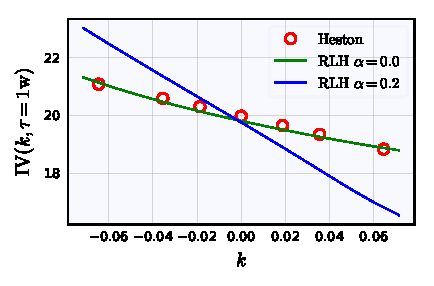
\includegraphics[height=0.32\linewidth]{figures/smile_skewed_1w}
    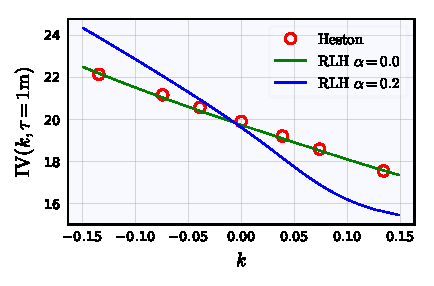
\includegraphics[height=0.32\linewidth]{figures/smile_skewed_1m}
    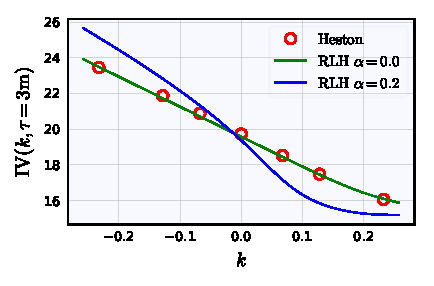
\includegraphics[height=0.32\linewidth]{figures/smile_skewed_3m}
    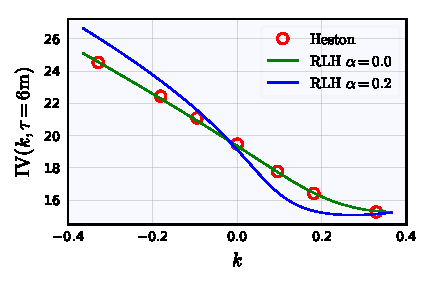
\includegraphics[height=0.32\linewidth]{figures/smile_skewed_6m}
    \hspace*{-2mm}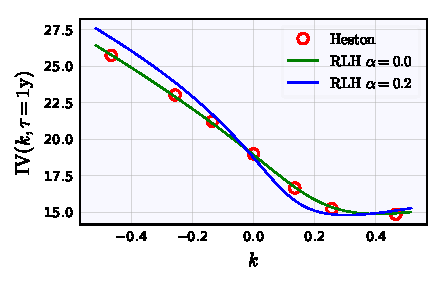
\includegraphics[height=0.32\linewidth]{figures/smile_skewed_1y}
    \hspace*{-2mm}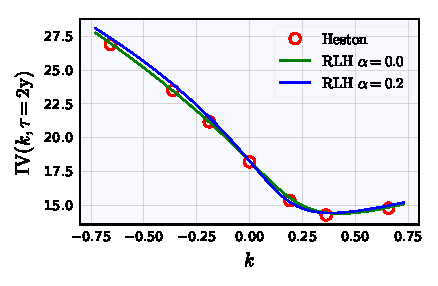
\includegraphics[height=0.32\linewidth]{figures/smile_skewed_2y}
    \caption{Implied volatilities $\mathrm{IV}(k,\tau)$ from the classical Heston and RLH models, defined in \autoref{eq:heston_plots} and \autoref{eq:RLH_plots} respectively, are shown. Parameters are set to $\sigma = \kappa = 0.2$, $\theta=v=0.04$, $\rho=-0.7$, with the fractional derivative $\alpha$ as shown.}
    \label{fig:heston_comparison_skewed}
\end{figure}

\vspace{4mm}

\begin{figure}[H]
    \centering
    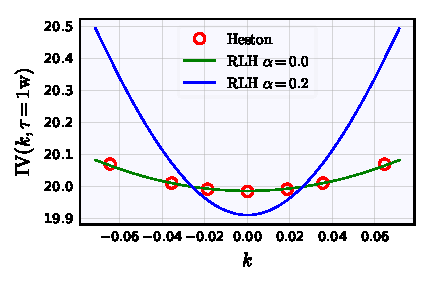
\includegraphics[height=0.32\linewidth]{figures/smile_symmetric_1w}
    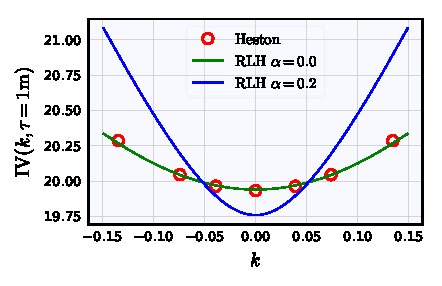
\includegraphics[height=0.32\linewidth]{figures/smile_symmetric_1m}
    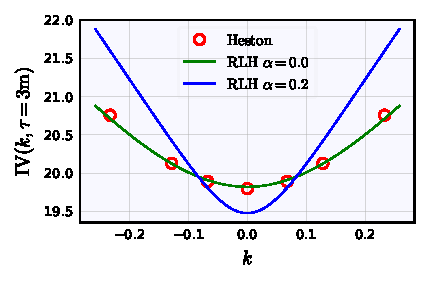
\includegraphics[height=0.32\linewidth]{figures/smile_symmetric_3m}
    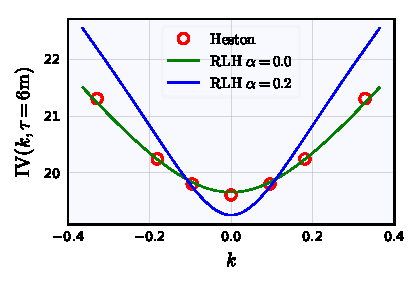
\includegraphics[height=0.32\linewidth]{figures/smile_symmetric_6m}
    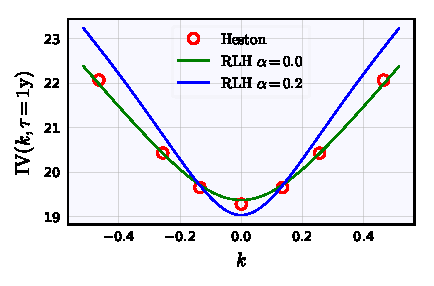
\includegraphics[height=0.32\linewidth]{figures/smile_symmetric_1y}
    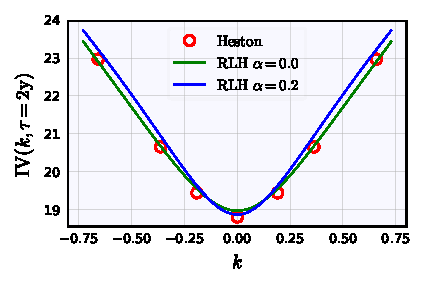
\includegraphics[height=0.32\linewidth]{figures/smile_symmetric_2y}
    \caption{A reproduction of \autoref{fig:heston_comparison_skewed} is shown, setting instead $\rho=0$.}
    \label{fig:heston_comparison_symmetric}
\end{figure}

\vspace{-4mm}

In both \autoref{fig:heston_comparison_skewed} and \autoref{fig:heston_comparison_symmetric}, the RLH implied volatilities clearly coincide with those of the classical Heston model when $\alpha=0$, validating \autoref{thm:heston_ode}. Given that all implied volatilities are similar for the two year maturity, the effect on shorter maturities when increasing $\alpha$ to 0.2 is also clear: in \autoref{fig:heston_comparison_skewed}, we observe increasingly pronounced skews as maturities fall to a week, and in \autoref{fig:heston_comparison_symmetric}, we observe increasingly pronounced curvatures.

Now in \autoref{fig:skews} and \autoref{fig:curvatures} we approximate (at-the-money) skews and curvatures by finite difference, defined for each maturity $\tau$ via the following absolute partial derivatives
\begin{equation}\label{eq:skew_curv}
    \mathrm{skew}(\tau):=\left|\frac{\partial\mathrm{IV}(k,\tau)}{\partial k}\right|_{k=0},\quad \mathrm{curvature}(\tau):=\left|\frac{\partial^2\mathrm{IV}(k,\tau)}{\partial k^2}\right|_{k=0}.
\end{equation}

\vspace{-4mm}

\begin{figure}[H]
    \centering
    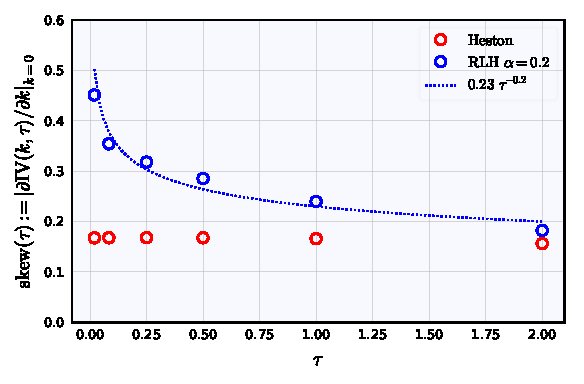
\includegraphics[width=0.75\linewidth]{figures/skew}
    \caption{At-the-money implied volatility skews approximated by central finite difference from the data in \autoref{fig:heston_comparison_skewed}.}
    \label{fig:skews}
\end{figure}

\vspace{-8mm}

\begin{figure}[H]
    \centering
    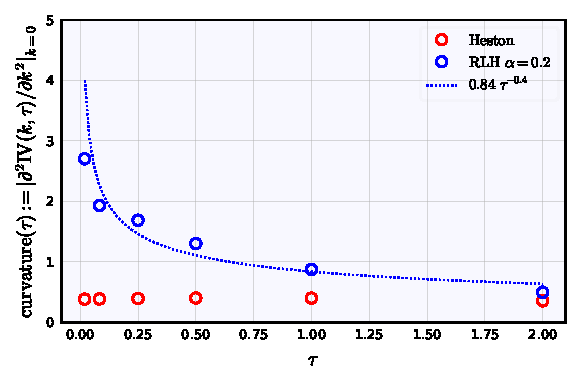
\includegraphics[width=0.74\linewidth]{figures/curvature}
    \caption{At-the-money implied volatility curvatures approximated by central finite difference from the data in \autoref{fig:heston_comparison_symmetric}.}
    \label{fig:curvatures}
\end{figure}

In \autoref{fig:skews} and \autoref{fig:curvatures} we hope to observe power law skews and curvatures, like those generated by leading rough volatility models, and considered a `stylised fact' of equity markets. We thus include power laws of type $\tau^{-\alpha}$ and $\tau^{-2\alpha}$ respectively, which are those predicted by the theory of \cite{alos_2007} and \cite{alos_2017} when translating the Hurst parameter $H$ there to our fractional derivative $\alpha$ via H\"older regularities, i.e.~$H=0.5-\alpha$. Despite these power laws being (short-time) approximations themselves, similarities between them and our finite difference RLH skews and curvatures are still clearly evident, suggesting that the RLH model indeed behaves like the leading rough volatility models in this respect.

Now in \autoref{fig:rough_heston_comparison}, we simulate implied volatilities using a modified RLH model, which are similar to those from Figures 1 and 2 in \cite{eleuch_2019b}, i.e.~the rough Heston model.

\begin{figure}[H]
    \centering
    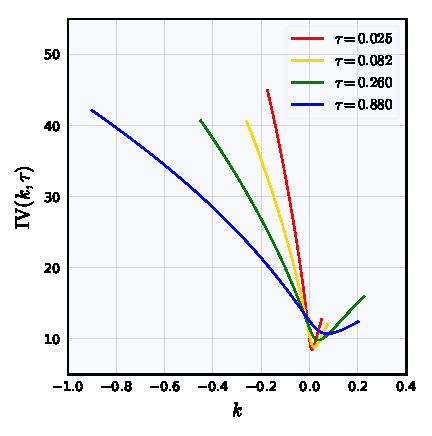
\includegraphics[width=0.48\linewidth]{figures/rough_heston_1}
    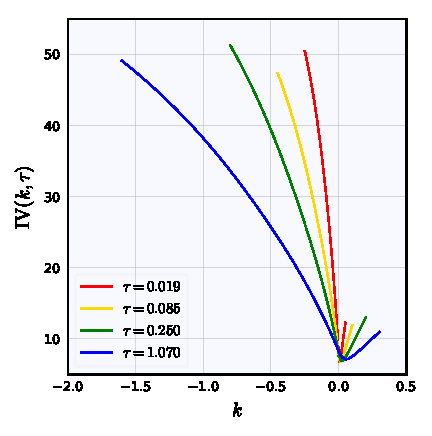
\includegraphics[width=0.48\linewidth]{figures/rough_heston_2}
    \caption{Implied volatilities from the modified RLH model in \autoref{eq:rough_heston_RLH}, which compare to those of rough Heston. Parameters are $H=0.1216,\nu=0.2910,\rho=-0.6714$ in the left panel and $H=0.0474,\nu=0.4061,\rho=-0.6710$ in the right.}
    \label{fig:rough_heston_comparison}
\end{figure}

\vspace{-4mm}

Contrasting the classical Heston variance process in \autoref{eq:heston_plots}, the rough Heston counterpart in \cite{eleuch_2019b} is a weak solution of the singular stochastic Volterra equation~
\begin{equation}\label{eq:rough_heston}
    V_t = \xi(t) + \frac{\nu}{\Gamma(H+\frac12)}\int_0^t(t-s)^{H-\frac12}\sqrt{V_s}\dd W^1_s,
\end{equation}
for a forward variance curve $\xi(t)=\EE[V_t]$, $H\in(0,\frac12)$ and $\nu>0$. For a comparison with the RLH model, we thus modify the cumulative variance process $X$ in \autoref{def:RLH_model} to solve
\begin{equation}\label{eq:rough_heston_RLH}
    X'_t = \vt(t) + \nu W^{\frac12-H}_{X_t}\ \  \iff\ \  V_t = \vt(t) + \frac{\nu}{\Gamma(H+\frac12)}\left(\int_0^{\cdot}(\cdot-x)^{H-\frac12}\dd W^1_x\right)_{\int_0^t V_s\dd s},
\end{equation}
where $V:=X'$, we allow $\vt(0)>0$, we have prioritised the rough Heston Hurst parameter $H=\frac12-\alpha$, and have removed the drift component $-X_t$ from \autoref{eq:RLH_model_summary} entirely. We note that this model has a unique (strong) solution by \autoref{thm:rand_well_posed} provided $\vt$ is strictly increasing. However, our martingality result depending on \autoref{cor:gauss_heston_mgf} no longer applies given this drift $-X_t$ is removed. This is practically irrelevant, however, because it \emph{does} apply if a drift $-\ep X_t$ is included in the r.h.s.~of \autoref{eq:rough_heston_RLH} for \emph{any} $\ep>0$, e.g.~$\ep:=2^{-100}$.

There are clear similarities between the rough Heston model in \autoref{eq:rough_heston} and our modified RLH model in \autoref{eq:rough_heston_RLH}. This is validated by \autoref{fig:rough_heston_comparison}, especially because this figure is produced \emph{not} by \emph{calibrating} our parameters $H,\nu,\rho$ to replicate the rough Heston output, but by simply adopting the rough Heston parameters from \cite{eleuch_2019b}. Note however that the RLH model produces higher implied volatilities in the left tails in \autoref{fig:rough_heston_comparison} in general, so there is still room for improvement through an actual calibration. Recalling \autoref{eq:theta_curve}, it remains to ensure the equivalence $\vt(t)=\xi(t) - \nu\EE[W^{\frac12-H}_{X_t}]$ to reasonable accuracy. We manage this on the fly during the simulation producing \autoref{fig:rough_heston_comparison}, but we find that curves of type $\vt(t)=\vt_0+\vt_1(1-2H)t^{2H}$ also produce reasonable output.

\vspace{2mm}

Through \autoref{fig:skews}, \autoref{fig:curvatures} and \autoref{fig:rough_heston_comparison}, we have thus provided convincing evidence that the RLH model behaves like the leading rough volatility models. However, more theoretical or numerical evidence is required to validate a relationship with the rough Heston model, given that our simulations producing \autoref{fig:rough_heston_comparison} depend on very high fractional derivatives. We clarify some potential future research regarding the RLH model at the end of \autoref{chap:conclusion}.

Finally, recall from the beginning of this chapter that our primary objective when defining the RLH model was to promote understanding for the wider volatility modelling frameworks in \autoref{fig:venn}, via the familiar \emph{classical} Heston model. These apparent \emph{rough} Heston similarities are a bonus. Unlike the rough Heston model, the RLH model exists in a framework where all models can be flexibly modified without compromising their unique strong solution, and have a continuous solution map w.r.t.~uniform convergence over compacts. Conditions for the rough Heston model (and related stochastic Volterra equations) to have a unique strong solution are still not yet known, despite attempts. The rough Heston model has a characteristic function which can be approximated, however, enabling semi-analytic pricing.

\subsection{Fractional Heston-NIG limits}\label{sec:price_limits}

In this final section the plan is to apply the limiting results from \autoref{chap:solutions}, most notably \autoref{thm:exit_limit}, to the RLH model from \autoref{def:RLH_model}. After doing so, we will demonstrate some surprising classical CIR and Heston limiting results as a special case. The former will establish an entirely new connection between the time-integrated CIR process and the IG L\'evy process, a consequence of which is the weak convergence on Skorokhod's $\uM_1$ topology.

The latter results will strengthen the Heston and NIG relationship discussed at length in the \hyperlink{prologue}{Prologue}. Recall that connections were already established in \cite{keller-ressel_2011} and \cite{forde_2011} between the Heston process for large times and the NIG \emph{distribution}, and \autoref{thm:mech_pro} from \cite{mechkov_2015} established the first connection between the marginal distributions of \emph{processes}. The Heston and NIG relationships here are therefore the first \emph{functional} results, illustrating how these processes are related (and not related, as it turns out) for all times simultaneously. These results are not as accessible as the CIR-related ones, with weak convergence being violated on all of Skorokhod's five topologies, for example.

To draw these conclusions on the classical CIR and Heston processes, the relationship from \autoref{thm:heston_ode} between these processes and the RLH model, when setting the fractional derivative $\alpha=0$, will be used. So recall the RLH model for an $\cF_{X_t}$-martingale price process $S=\{S_t\}_{t\in\RR_+}$ and its cumulative variance $X=\{X_t\}_{t\in\RR_+}$, summarised by the equations
\begin{equation}\label{eq:RLH_model_limit}
    X'_t = \sigma W^\alpha_{X_t} + \kappa(\vt(t) - X_t) + v,\quad S_t=\exp(W^\rho_{X_t}-\tfrac12 X_t),
\end{equation}
where we define the usual processes $W^\alpha:=D^\alpha(W^1)$ and $W^\rho:=\rho W^1+\sqrt{1-\rho^2}W^0$. We are now interested in sequences of such models which can be expressed just in terms of sequences of the implicit underlying random field in \autoref{eq:RLH_model_limit}. Specifically, we consider fields
\begin{equation}\label{eq:RLH_field_seq}
    Y^n_{t,x} := \sigma_n W^\alpha_x + \kappa_n(\vt_n(t) - x) + v_n,
\end{equation}
noting that this means the Brownian motion $(W^0,W^1)$ and parameters $\alpha,\rho$ are now fixed.

When applying \autoref{thm:exit_limit} to such fields, the curves $\kappa_n\vt_n(t)+v_n$ play the same role provided a limit is found uniformly over compacts as $n\to\infty$, so in order to help draw direct conclusions on the classical CIR and Heston processes we will just consider the (classical) cases of $\vt_n(t):=\theta t$ and $v_n:=v$ for $\theta,v>0$. Fields in \autoref{eq:RLH_field_seq} can thus be expressed
\begin{equation}\label{eq:RLH_model_limit2}
    Y^n_{t,x} := \sigma_n W^\alpha_x + \kappa_n(\theta t - x) + v
\end{equation}
and in the results which follow, the term $\theta t$ can be generalised to a limiting curve $\vt_0(t)$.

Recall from \autoref{thm:heston_ode} that when we set the fractional derivative $\alpha=0$ in \autoref{eq:RLH_model_limit2}, the distribution of the random ODE solution $X$ coincides with that of an integrated CIR process, and that of $S$ with a Heston price process. Now depending on how we let $\sigma_n$ and $\kappa_n$ scale with $n$, different, possibly discontinuous, limits will be obtained via \autoref{thm:exit_limit}.

We are most interested here in limits like those studied in \cite{mechkov_2015} and summarised in the \hyperlink{prologue}{Prologue}, where $\sigma_n,\kappa_n\xrightarrow{n\to\infty}\infty$ at the same rate, because we know these lead to the most informative and practically useful functional relationships between classical processes. In the \hyperlink{epilogue}{Epilogue}, clarity is provided on alternative limits deriving from the regimes of \cite{heston_1993} and \cite{fouque_2011}, also accommodating the case where $Y^n_{0,0} = v_n\xrightarrow{n\to\infty}\infty$.

\vspace{3mm}\textbf{The fast-reversion parameterisation.} In \cite{mechkov_2015} a particular `fast-reversion' parameterisation of the Heston model is defined which, subject to a relabelling of the parameters $a,b,c>0$, amounts to considering the following It\^o SDEs indexed by any $n>0$~
\begin{equation}\label{eq:fast_reversion_heston}
    \dd V^n_t = na\sqrt{V^n_t}\dd W^1_t + n(b - V^n_t),\quad \dd S^n_t = \sqrt{V^n_t}S^n_t\dd W^\rho_t,\quad (V^n_0,S^n_0)=(c,1).
\end{equation}
The novelty of this parameterisation is due to the linear scaling of \emph{both} the  diffusion and reversion components of the CIR SDE for $V$ with $n$. Through an analysis of characteristic functions (given the system in \autoref{eq:fast_reversion_heston} is affine), the convergence in distribution $S^n_t\xrightarrow{\mathrm{d}}S^0_t$ is obtained as $n\to\infty$ for any $t>0$, where $S^0$ is an exponentiated NIG L\'evy process, with parameters depending only on $a,b$ and $\rho$ and no longer $c$. This result is summarised by \autoref{thm:mech_pro}, will be confirmed by \autoref{cor:heston_fd} then extended in \autoref{cor:heston_hausdorff}. Now we want to parameterise a sequence of RLH models in a similar `fast-reversion' way.

Considering how the RLH model is connected with the classical Heston model, through \autoref{thm:heston_ode}, such a parameterisation like that in \autoref{eq:fast_reversion_heston} is achieved by utilising fields $Y^n$ as in \autoref{eq:RLH_model_limit2} with $\sigma_n:=na$ and $\kappa_n:=n$. This leads simply to the following.

\begin{definition}[Fast-reversion RLH parameterisation]\label{def:fast_RLH}
    In the RLH model from \autoref{def:RLH_model}, set $\sigma=na$, $\kappa=n$, $\vt(t)=b t$ and $v=c$ for some $n,a,b,c>0$, so that the RLH processes $(X^n,S^n)$ are the unique processes over $\RR_+$ which verify the defining equations
    \begin{equation}\label{eq:RLH_model_summary3}
        {X^n_t}' = n\left( a W^\alpha_{X^n_t} + b t - X^n_t\right) + c,\quad S^n_t=\exp\left(W^\rho_{X^n_t}-\tfrac12 X^n_t\right),
    \end{equation}
    for some fixed $\alpha\in(0,\frac12)$ and $\rho\in[-1,1]$. We will say that such an RLH model is in its fast-reversion parameterisation, and will call $n\to\infty$ the RLH model's fast-reversion limit.
\end{definition}

Now our main focus is on establishing a.s.~functional limits of this model via the probability-free results of \autoref{chap:solutions}. Then, by setting $\alpha=0$, these will immediately provide weak limits for the Heston model as in \autoref{eq:fast_reversion_heston}. Although we are interested in a.s.~limits of the RLH model in their own right, notice how the approach here to weak convergence for the classical Heston model contrasts the usual `Prokhorov approach' via finite-dimensional distributions and tightness, as summarised succinctly e.g.~in \cite{jacod_2003}.

On all topologies from \cite{skorokhod_1956}, a naive application of Prokhorov's approach to the Heston price process in \autoref{eq:fast_reversion_heston} is doomed, because the functional limits established here go via \autoref{cor:graph_hausdorff}; these are not continuous process limits, not c\`adl\`ag processes, but compact \emph{interval-valued} processes, with paths $\ve(t)=:[\ve_-(t),\ve_+(t)]$ in the set $\uE$ from \autoref{def:excursionary_paths}. Such processes are studied in Chapter 15 of \cite{whitt_2002}, and their emergence here in finance is not just theoretically fascinating, but practically valuable, given they characterise unexpected behaviour of path-dependent derivatives, discussed in \autoref{chap:conclusion}.

\vspace{3mm}\textbf{Preparatory results.} All of the stochastic process limits of this section derive from the probability-free results from \autoref{sec:bounds_limits} and \autoref{sec:excursionary_limits}. Specifically, we will apply the exit-time and Hausdorff results of \autoref{thm:exit_limit} and \autoref{cor:graph_hausdorff}. So that the application of these results are clear, we first clarify their consequences in the probabilistic setting here.

Recall the set $\bPhi\subset\uD(\RR_+,\RR_+)$ from \autoref{def:setE}, containing the strictly increasing and unbounded c\`adl\`ag paths, and let $d_{\bPhi}$ be the exit-time metric from \autoref{def:exit_metric} satisfying $d_{\bPhi}(\bvp_1,\bvp_2) = \Vert E(\bvp_2) - E(\bvp_1)\Vert_{\RR_+}$. For clarity, $E$ is the exit-time functional from \autoref{def:exit_functional}, and $\Vert\cdot\Vert_{\RR_+}$ is the norm from \autoref{def:uni_metric}, characterising uniform convergence over compacts. Finally recall the set $\uG\subset\uC(\RR_+^2,\RR)$ from \autoref{def:mod_driving_func}, featuring in \autoref{prob:random_ivp}.

The proof of this next result is not given because it is identical to that of point 3.~in \autoref{thm:rand_well_posed}, only replacing the pathwise application of \autoref{thm:wellposed} with that of \autoref{thm:exit_limit}.

\begin{corollary}[Uniform exit-time limits]\label{cor:exit_limit}
    Let $\{Y^n\}_{n\in\NN_0}$ be random fields in $\uG$, let $\{X^n\}_{n\in\NN}$ solve the random IVPs $x'=nY^n_{t,x}$, $x_0=0$ and define $X^0\in\bPhi$ by $X^0_t:=\inf\{x>0:Y^0_{t,x}<0\}$. If $Y^n \xrightarrow[n\to\infty]{\mathrm{a.s.}}Y^0$ uniformly over compacts, then $X^n \xrightarrow[n\to\infty]{\mathrm{a.s.}} X^0$ on the exit-time space $(\bPhi,d_{\bPhi})$.
\end{corollary}

As covered by \autoref{thm:m1_relationship} and \autoref{cor:ae_converge}, recall that this convergence $X^n \to X^0$ on $(\bPhi,d_{\bPhi})$ is stronger than the same on Skorokhod's $\uM_1$ space (defined via the metric in \autoref{eq:m1_metric}) as well as providing the a.s.~pointwise convergence for (Lebesgue) a.e.~$t\in\RR_+$.

Now \autoref{cor:graph_hausdorff} translated into our probabilistic setting provides the following on $(\uE,d_\uE)$, where we recall from \autoref{def:excursionary_paths} that $\uE$ is the set of compact interval-valued paths over $\RR_+$, and $d_\uE$ the Hausdorff metric on this set, defined via the pseudometrics in \autoref{eq:hausdorff_dist}. In the following, we allow processes $\Lambda_X\in\uE$ to return the singleton $\{\Lambda_{X_t}\}$ for each $t\in\RR_+$.

\begin{corollary}[Hausdorff composite limits]\label{cor:hausdorff_random}
    Adopt the assumptions of \autoref{cor:exit_limit}, so that $X^n \xrightarrow[n\to\infty]{\mathrm{a.s.}} X^0$ on $(\bPhi,d_{\bPhi})$, and let $\Lambda=\{\Lambda_x\}_{x\in\RR_+}$ be any process in $\uC(\RR_+,\RR)$. Then the composition processes $\{\Lambda\circ X^n:=\Lambda_{X^n}\}_{n\in\NN}$ verify $\Lambda\circ X^n \xrightarrow[n\to\infty]{\mathrm{a.s.}} \Lambda\bullet X^0$ on $(\uE,d_\uE)$, where
    \begin{equation}
        (\Lambda\bullet X^0)_t := \{\Lambda_x:x\in[X^0_{t_-},X^0_t]\}.
    \end{equation}
\end{corollary}

Recall that the proof of \autoref{cor:graph_hausdorff}, on which \autoref{cor:hausdorff_random} here depends, goes via \autoref{thm:para_uniform}, which is not just a graphical Hausdorff convergence result, but a product convergence result for \emph{specific} parametric representations which \emph{generate} these graphs. The corresponding product statement giving \autoref{cor:hausdorff_random} here is $((X^n)^{-1},\Lambda)\to(E(X^0),\Lambda)$ uniformly over compacts. Although stronger, this does not lead to direct statements on our models, but rather on higher-dimensional representations of them. These representations may be helpful in the future, but for now we prefer to prioritise the likes of \autoref{cor:hausdorff_random}.

Now we are ready to apply these results to understand the fast-reversion limit of the RLH processes $X^n$ and $S^n$ in \autoref{def:fast_RLH}. Indeed, similarities between $\Lambda\bullet X$ in \autoref{cor:hausdorff_random} and our NIG generalisation $S^\bullet$ from \autoref{eq:ex_nig_pro} in the \hyperlink{prologue}{Prologue} should already be evident.

\vspace{3mm}\textbf{Cumulative variance limits.} We now characterise a limit $X^0$ of a sequence of the processes $X^n$ from \autoref{def:fast_RLH} as $n\to\infty$, i.e.~the RLH fast-reversion limit. \autoref{cor:exit_limit} will be applied to establish these, so despite each process $X^n$ being differentiable, the limit $X^0$ will exhibit discontinuities, like the following generalisation of the IG L\'evy process. Recall the Riemann-Liouville (RL) fractional derivative process $W^\alpha$ from \autoref{def:RL_process}.

\begin{definition}[Fractional IG process]\label{def:frac_IG}
    For $a,b>0$ and $\alpha\in(0,\frac12)$, define the RL fractional process $W^\alpha:=D^\alpha(W^1)$ as usual and the process $X^0=\{X^0_t\}_{t\in\RR_+}$ by the exit-time~
    \begin{equation}\label{eq:frac_IG}
        X^0_t :=\inf\big\{x>0 : x - a W^\alpha_x > bt\big\}.
    \end{equation}
    Such a process $X^0$ will be called a fractional IG process of order $\alpha$, with parameters $a,b$.
\end{definition}

By defining $\delta:=a^{-1}b$ and $\gamma:=a^{-1}$, this fractional IG process coincides precisely with the classical IG L\'evy process with parameters $\delta,\gamma>0$ as defined in \cite{applebaum_2009}, \emph{when} $\alpha=0$ (so when $W^\alpha$ is Brownian motion), which has MGF $e^{\delta(\gamma-\sqrt{\gamma^2-2u})t}$ in general, so $\EE[e^{pX^0_t}] = e^{ba^{-2}(1-\sqrt{1-2a^2u})t}$ in our case. As already discussed, this process could be further generalised via a suitable curve $\vt(t)$ in place of the linear exit-barrier $bt$ in \autoref{eq:frac_IG}.

Like the classical IG process, the fractional IG process has strictly increasing and unbounded c\`adl\`ag paths, but remains finite over $\RR_+$, so is a.s.~in $\bPhi$. This follows e.g.~from \autoref{lem:zeros2}, and \autoref{cor:gauss_heston_mgf}. This latter result actually establishes the MGF existence $M^0_X(p,t)=\EE[e^{pX^0_t}]<\infty$ for all $(p,t)\in\RR\times\RR_+$, from which a.s.~finiteness $X^0_t<\infty$ of course follows. Now applying \autoref{cor:exit_limit} to the RLH model yields the fractional IG process as follows.

\begin{corollary}[Fractional IG limits]\label{cor:frac_IG_limit}
    Let $\{X^n\}_{n\in\NN}$ be a sequence of RLH processes as in \autoref{def:fast_RLH}, and let $X^0$ be the fractional IG process from \autoref{def:frac_IG}, so that
    \begin{equation}\label{eq:frac_ig_sum}
        {X^n_t}' = n\left( a W^\alpha_{X^n_t} + b t - X^n_t\right) + c,\quad X^0_t =\inf\big\{x>0 : x - a W^\alpha_x > bt\big\}.
    \end{equation}
    Then the convergence $d_{\bPhi}(X^n,X^0)=\Vert E(X^0) - (X^n)^{-1}\Vert_{\RR_+}\asc 0$ takes place as $n\to\infty$.
\end{corollary}
\begin{proof}
    The processes $\{X^n\}_{n\in\NN}$ each solve the random IVPs $x'=n Y^n_{t,x}$, $x_0=0$, where
    \begin{equation}
        Y^n_{t,x} := a W^\alpha_x + b t - x + n^{-1}c,
    \end{equation}
    and clearly $Y^n\asc Y^0$ uniformly over compacts of $\RR_+^2$ as $n\to\infty$, where $Y^0_{t,x}:=a W^\alpha_x + b t - x$. All of the RLH fields $\{Y^n\}_{n\in\NN_0}$ are moreover in $\uG$, as confirmed following the MGF existence in \autoref{cor:rlh_mgf_exist}. So the assumptions of \autoref{cor:exit_limit} hold, and we therefore obtain the convergence $X^n \asc X^0$ on $(\bPhi,d_{\bPhi})$, where $X^0\in\bPhi$ is defined by $X^0_t:=\inf\{x>0:Y^0_{t,x}<0\}$. Since this expression for $X^0$ coincides with that in \autoref{eq:frac_ig_sum}, the proof is complete.
\end{proof}

Now recall from \autoref{thm:m1_relationship} that convergence on the exit-time space $(\bPhi,d_{\bPhi})$ is stronger than on Skorokhod's $\uM_1$ space, essentially because the former considers only distances \emph{in time} between paths, rather than both time and space. In turn, like in \autoref{cor:ae_converge}, we get a.s.~(Lebesgue) a.e.~pointwise convergence. That is, for all times $T\in\RR_+$, we a.s.~have
\begin{equation}
    \mathrm{Leb}\left[t\in[0,T]: X^n_t\xrightarrow{n\to\infty}X^0_t\right]=T.
\end{equation}

Finally note that the limiting exit-time process $E(X^0)$ appearing in \autoref{cor:frac_IG_limit} was analysed in \cite{vellaisamy_2018} in the non-fractional case $\alpha=0$. Using the relationship $E\circ E=M$ noted in \autoref{lem:whitt}, this may be equivalently expressed using the maximal functional from \autoref{eq:maximal_func}, as $E(X^0)=b^{-1}M(\id-aW^\alpha)$, i.e.~$E(X^0)_x=b^{-1}\max_{u\in[0,x]}\{u-aW^\alpha_u\}$. The inverses $\{(X^n)^{-1}\}_{n\in\NN}$ in \autoref{cor:frac_IG_limit} a.s.~find this maximal limit uniformly over compacts, which can be observed on a pathwise basis e.g.~in \autoref{fig:exit_converge}.

\vspace{3mm}\textbf{Classical integrated CIR limits.} Now we clarify what \autoref{cor:frac_IG_limit}, connecting the RLH model with the fractional IG process, means for the classical CIR process in the Heston model from \autoref{eq:fast_reversion_heston}. Given the popularity of the CIR and IG processes in \autoref{cor:IG_limit}, it is surprising that even the 1d reduction of \autoref{cor:IG_limit_fd} is new, despite a large-time connection between a CIR process and IG distribution being known since \cite{tse_2013}. Accordingly, these results demonstrate our pathwise ODE-based framework's ability to teach us surprising new results about already much-analysed stochastic processes.

\begin{corollary}[Inverse-Gaussian exit-time limits]\label{cor:IG_limit}
    Let $\{V^n\}_{n\in\NN}$ be a sequence of CIR processes as in \autoref{eq:fast_reversion_heston}, and define $\{X^n\}_{n\in\NN}$ respectively by the time-integrals $X^n_t:=\int_0^t V^n_s\dd s$. Define also the IG process $X^0$ as in \autoref{def:frac_IG} with $\alpha=0$ so, in summary,
    \begin{equation}
        \dd V^n_t = na \sqrt{V^n_t}\dd W^1_t + n(b - V^n_t)\dd t,\quad V^n_0=c,\quad X^0_t =\inf\big\{x>0 : x - a W^1_x > bt\big\}.
    \end{equation}
    Then the weak convergence $X^n\cw X^0$ takes place on the exit-time metric space $(\bPhi,d_{\bPhi})$.
\end{corollary}
\begin{proof}
    To avoid a clash of notation, denote by $\{\tX^n\}_{n\in\NN}$ the processes $\{X^n\}_{n\in\NN_0}$ from \autoref{cor:frac_IG_limit} when setting $\alpha=0$, so we obtain $\tX^n \asc X^0$ on $(\bPhi,d_{\bPhi})$. As shown in \autoref{thm:heston_ode}, we then have the equivalence $\tX^n\ed X^n$ in distribution for every $n\in\NN$. (Given we have adopted the parameterisation in \autoref{def:fast_RLH}, note the parameter relationships there, e.g.~$\sigma=na$.) So from $\tX^n \asc X^0$ on $(\bPhi,d_{\bPhi})$ we obtain $X^n\cw X^0$ as claimed.
\end{proof}

This convergence on $(\bPhi,d_{\bPhi})$ is equivalent to the weak convergence $E(X^n)\cw E(X^0)$ of exit-times w.r.t.~uniform convergence over compacts. Like with \autoref{cor:frac_IG_limit}, convergence on Skorokhod's $\uM_1$ space takes place as a consequence, and now it is natural, and practically relevant, to ask whether we also have convergence of finite-dimensional distributions. This will be denoted $X^n\cfd X^0$ as $n\to\infty$, which means the weak convergence $(X^n_{t_1},\dots,X^n_{t_d})\cw(X^0_{t_1},\dots,X^0_{t_d})$ takes place for any $\{t_k\}_{k=1}^d\subset\RR_+$ of dimension $d\in\NN$.

As demonstrated in Chapter 13 of \cite{billingsley_1999}, this \emph{does not} follow even from weak convergence on Skorokhod's stronger $\uJ_1$ space, but does if the processes of concern have the property of stochastic continuity, i.e.~$\PP[X_{t_-}= X_t]=1$, where $X_{t_-}:=\lim_{s\uparrow t}X_s$ as usual, and in our setting $X_{0_-}:=0$. This next result shows that $X^n\cfd X^0$ as $n\to\infty$ similarly holds in our setting, provided $X^0$ is stochastically continuous, like any L\'evy process.

For the proof, recall that $\PP[X_{t_-}= X_t]=1$ provides also $\PP[X_{{t_k}_-}= X_{t_k},k=1,\dots,d]=1$ for any finite $\{t_k\}_{k=1}^d\subset\RR_+$, which can be proved using the basic manipulations in \autoref{eq:full_measure}. Also recall from \autoref{cor:ae_converge} that convergence $\bvp_n\to\bvp_0$ on $(\bPhi,d_{\bPhi})$ provides also the pointwise convergence $\bvp_n(t)\to\bvp_0(t)$ for any point of continuity for $\bvp_0$, which is a.e.~at least. The same was shown in \cite{skorokhod_1956} to hold for all metrics defined there.

\begin{corollary}[Inverse-Gaussian f.d.~limits]\label{cor:IG_limit_fd}
    Supplementing \autoref{cor:IG_limit}, the convergence $X^n\cfd X^0$ of finite-dimensional distributions over $\RR_+$ also takes place as $n\to\infty$.
\end{corollary}
\begin{proof}
    Let $\{\tX^n\}_{n\in\NN}$ be as in the proof of \autoref{cor:IG_limit}, so that $\tX^n \asc X^0$ on $(\bPhi,d_{\bPhi})$ and $\tX^n\ed X^n$ for each $n\in\NN$. Recall that each $\tX^n$ is differentiable, and $X^0$ is an inverse-Gaussian L\'evy process, thus stochastically continuous. Fixing any finite set $\{t_k\}_{k=1}^d\subset\RR_+$, we therefore have $\PP[X^0_{{t_k}_-}= X^0_{t_k},k=1,\dots,d]=1$.  Since convergence on $(\bPhi,d_{\bPhi})$ provides convergence on $(\RR,|\!\cdot\!|)$ at points of continuity, then from $\tX^n \asc X^0$ on $(\bPhi,d_{\bPhi})$ and the a.s.~continuity $\PP[X^0_{{t_k}_-}= X^0_{t_k},k=1,\dots,d]=1$ we get $(\tX^n_{t_1},\dots,\tX^n_{t_d})\asc(X^0_{t_1},\dots,X^0_{t_d})$ on $(\RR^d,|\cdot|)$. Given $\tX^n\ed X^n$, this provides $(X^n_{t_1},\dots,X^n_{t_d})\cw(X^0_{t_1},\dots,X^0_{t_d})$. So the claim of $X^n\cfd X^0$ is established by definition, given the finite set $\{t_k\}_{k=1}^d\subset\RR_+$ is arbitrary.
\end{proof}

It is of course possible to verify \autoref{cor:IG_limit_fd}, given the integrated CIR and IG processes are affine, so have closed form MGF representations. Actually doing so in the 1d case is similar to the proof via MGFs given for \autoref{lem:int_cir_unbound}. For this let the processes $\{X^n\}_{n\in\NN_0}$ be those in \autoref{cor:IG_limit}, and for $2a^2p<1$ and $t>0$ define the MGFs $M^n_X(p,t):=\EE[e^{pX^n_t}]$. We then obtain $M^n_X(p,t) = e^{\vp^n_0(t)+\vp^n_1(t)c}$, where for $n\in\NN$ and $\lambda:=\sqrt{1-2a^2 p}>0$ we find
\begin{equation}\label{eq:IG_mgf1}
    \vp^n_0(t):= \frac{bt}{a^2}- \frac{2b}{a^2 n}\log\left(\cosh\left(\frac{n \lambda t}{2}\right) + \frac{1}{\lambda}\sinh\left(\frac{n \lambda t}{2}\right)\right),\ \vp^n_1(t):= \frac{2pn^{-1}}{1 + \lambda\coth\left(\frac{n \lambda t}{2}\right)}.
\end{equation}
Subject to redefining parameters, these expressions coincide with those given in \autoref{eq:int_cir_char_func}. From \autoref{eq:IG_mgf1} we can see $\vp_1^n(t)\xrightarrow{n\to\infty}\vp_1^0(t) := 0$ provided $\lambda>0$, which is ensured by $2a^2p<1$. Using similar expansions to those given in \autoref{lem:int_cir_unbound}, we also find
\begin{equation}
    \frac{2}{n}\log\left(\cosh\left(\frac{n \lambda t}{2}\right) + \frac{1}{\lambda}\sinh\left(\frac{n \lambda t}{2}\right)\right)\xrightarrow{n\to\infty}\lambda t.
\end{equation}
So in full we find $\vp_0^n(t)\xrightarrow{n\to\infty}\vp_0^0(t) := ba^{-2}(1 - \lambda)t$, and the resulting MGF limit $M^0_X(p,t) = e^{\vp^0_0(t)+\vp^0_1(t)c} = e^{ba^{-2}(1-\lambda)t} = e^{ba^{-2}(1-\sqrt{1-2a^2 p})t}$ is that of the IG random variable $X^0_t$ from \autoref{cor:IG_limit_fd}, as clarified after \autoref{def:frac_IG}. This reconciles \autoref{cor:IG_limit_fd} in the 1d case, and doing so in higher dimensions is possible via induction, although rather tedious. This contrasts our proof of \autoref{cor:IG_limit_fd}, which can even be visualised like in \autoref{fig:exit_converge}.

Since this result relating the classical integrated CIR and IG processes is just one of the limits arising when applying \autoref{thm:exit_limit}, we clarify in the \hyperlink{epilogue}{Epilogue} all the other limits that can arise when the CIR processes are parameterised differently. These include the \emph{L\'evy} L\'evy process which, as \cite{applebaum_2009} shows, can be considered a special case of the IG L\'evy process, and both of these L\'evy processes can also arise with random starting points.

\vspace{3mm}\textbf{Price process limits.} In this part we will conduct the same type of analysis as the previous but for the RLH \emph{price} processes $S^n$ in \autoref{def:fast_RLH}. Then in the next part, we will reduce this to consequences for the classical Heston model from \autoref{eq:fast_reversion_heston}, finally strengthening \autoref{thm:mech_pro} as far as we deem possible and thereby answering our questions in the \hyperlink{prologue}{Prologue}.

As with the fractional IG process from \autoref{def:frac_IG}, we first define \emph{two} candidate limits of the RLH price processes. The senses in which these generalise the classical NIG process, see e.g.~\cite{barndorff-nielsen_2001a}, \cite{cont_2003} or \cite{applebaum_2009}, will be clarified in the next part, when these limits are related to the classical Heston model.

\begin{definition}[Fractional NIG c\`adl\`ag process]\label{def:frac_NIG1}
    Let $X^0$ be the fractional IG process from \autoref{def:frac_IG}, then define the process $S^\circ=\{S^\circ_t\}_{t\in\RR_+}$ as in \autoref{eq:RLH_model_summary3}. So in full,
    \begin{equation}
        X^0_t:=\inf\big\{x>0:x-aW^\alpha_x>bt\big\},\quad S^\circ_t:=\exp\left(W^\rho_{X^0_t}-\tfrac12 X^0_t\right),
    \end{equation}
    for $a,b>0$, $\alpha\in(0,\frac12)$, $\rho\in[-1,1]$, with $W^\alpha:=D^\alpha(W^1)$ and $W^\rho:=\rho W^1+\sqrt{1-\rho^2}W^0$ as usual. $S^\circ$ will be called a fractional NIG \emph{c\`adl\`ag} process of order $\alpha$, with parameters $a,b,\rho$.
\end{definition}

Given $\exp(W^\rho_x-\tfrac12 x)$ is a continuous process over $\RR_+$ and $X^0$ a strictly increasing c\`adl\`ag process over $\RR_+$ with $X^0_0=0$, it is clear that $S^\circ$ is indeed a c\`adl\`ag process over $\RR_+$, with $S^\circ_0=1$. Note that an alternative `Fractional NIG' process is studied in the line of research from \cite{kumar_2012} to \cite{wylomanska_2016}, considered for several applications in statistical physics. In this alternative case, fractional Brownian motion is being subordinated, whereas our fractional process $W^\alpha$ is hidden \emph{within} our volatility-related subordinator $X^0$. So the emergence of our candidate limit $S^\circ$ from a sequence of martingales remains plausible. We now define a related \emph{interval-valued} process.

\begin{definition}[Fractional NIG excursion process]\label{def:frac_NIG2}
    Let $a,b,\alpha,\rho,W^0,W^1$ and $X^0$ be as in \autoref{def:frac_NIG1}, but define the real interval-valued process $S^\bullet=\{S^\bullet_t\}_{t\in\RR_+}$ instead using
    \begin{equation}\label{eq:frac_NIG_ex}
        S^{\bullet}_t:=\left\{\exp\left(W^\rho_x-\tfrac12 x\right):x\in[X^0_{t_-},X^0_t]\right\}.
    \end{equation}
    Then $S^\bullet$ will be called a fractional NIG \emph{excursion} process of order $\alpha$, with parameters $a,b,\rho$.
\end{definition}

Again, by the continuity of $\exp(W^\rho_x-\tfrac12 x)$, each $S^\bullet_t$, for $t\in\RR_+$, defines a random \emph{closed subinterval} of $\RR$, not just a random subset. Indeed, we have the equivalent representation
\begin{equation}\label{eq:frac_NIG_ex2}
    S^\bullet_t=\left[\min_{x\in[X^0_{t-},X^0_t]}\exp(W^\rho_x-\tfrac12 x),\max_{x\in[X^0_{t-},X^0_t]}\exp(W^\rho_x-\tfrac12 x)\right]=:[S^-_t,S^+_t].
\end{equation}
It is clear from these expressions that these c\`adl\`ag and excursion processes satisfy $S^\circ_{t_-},S^\circ_t\in S^\bullet_t$ for each $t\in\RR_+$. We should think of $S^\bullet$ as being equivalent to $S^\circ$, only with additional instantaneous excursions attached at the times of the discontinuities of $X^0$ (when $X^0_{t-}<X^0_t$), thus $S^\circ$. The upwards excursions have length $S^+_t-S^\circ_t\ge0$, and the downward excursions $S^\circ_t-S^-_t\ge0$, and both are a.s.~zero at a fixed time, meaning $S^-_t=S^\circ_t=S^+_t$, provided $X^0$ is stochastically continuous. Like the discontinuities of any c\`adl\`ag process such as $X^0$ and $S^\circ$, these excursions are a.s.~countable along a given path, so regardless of stochastic continuity we a.s.~have $S^\bullet_t=\{S^\circ_t\}$ for a.e.~$t\in\RR_+$, meaning again $S^\circ_t=S^-_t=S^+_t$.

Such an interval-valued process $S^\bullet$, connected with a specific c\`adl\`ag process $S^\circ$, falls beautifully into the setting of Section 15.4 in \cite{whitt_2002}, arising in queuing theory. Like in \autoref{cor:hausdorff_random}, we will consider $S^\bullet$ as a random element of $\uE$ from \autoref{def:excursionary_paths}. Recall that $\uE$ simply contains \emph{all} real compact interval-valued paths over $\RR_+$, i.e.~not just those of $S^\bullet$ which are connected to the c\`adl\`ag paths of $S^\circ$. It is with respect to the Borel $\sigma$-algebra $\cE$ induced by the excursionary (Hausdorff) metric $d_\uE$ from \autoref{def:excursionary_metric} on $\uE$ that we can consider $S^\bullet$ a bona fide stochastic process, i.e.~a measurable map from $(\Omega,\cF,\PP)$ to $(\uE,\cE)$.

The next two results clarify notions in which a sequence $\{S^n\}_{n\in\NN}$ of RLH price processes from \autoref{def:fast_RLH} converge to the fractional NIG processes $S^\circ$ and $S^\bullet$ respectively. These results constitute straightforward applications of \autoref{cor:ae_composite} and \autoref{cor:hausdorff_random} respectively.

\begin{corollary}[A.e.~fractional NIG limits]\label{cor:price_ae}
    Let $\{S^n\}_{n\in\NN}$ be a sequence of RLH price processes from \autoref{def:fast_RLH}, and $S^\circ$ the fractional NIG c\`adl\`ag process from \autoref{def:frac_NIG1}. Then a.s., the convergence $S^n_t\xrightarrow{n\to\infty}S^\circ_t$ takes place a.e., i.e. for all $T\in\RR_+$, we a.s.~have
    \begin{equation}
        \mathrm{Leb}\left[t\in[0,T]: S^n_t\xrightarrow{n\to\infty}S^\circ_t\right]=T.
    \end{equation}
\end{corollary}
\begin{proof}
    Given $X^n\asc X^0$ on $(\bPhi,d_{\bPhi})$ from \autoref{cor:frac_IG_limit} and that $\Lambda_x:=\exp(W^\rho_x-\frac12 x)$ a.s.~has paths in $\uC(\RR_+,\RR)$, then applying \autoref{cor:ae_composite} on a pathwise basis a.s.~provides
    \begin{equation}
        \Leb\left[t\in[0,T]:\Lambda_{X^n_t}\xrightarrow{n\to\infty}\Lambda_{X^0_t}\right]=T.
    \end{equation}
    But now just using the definitions of $S^n$, $S^\circ$ and $\Lambda$, we see that this is precisely the claim.
\end{proof}

Although this limiting result is sufficient for some applications, the following is necessary to understand the richer limiting behaviour of path-dependent derivatives. Like in \autoref{cor:hausdorff_random}, we let $S^n$ simultaneously denote the process in $\uE$ returning the singletons $\{S^n_t\}$.

\begin{corollary}[Hausdorff fractional NIG limits]\label{cor:price_hausdorff}
    Let $\{S^n\}_{n\in\NN}$ be a sequence of RLH price processes from \autoref{def:fast_RLH}, and let $S^\bullet$ be the fractional NIG excursion process from \autoref{def:frac_NIG2}. Then the convergence $S^n\asc S^\bullet$ takes place on $(\uE,d_{\uE})$ as $n\to\infty$.
\end{corollary}
\begin{proof}
    Like in \autoref{cor:price_ae}, define the process $\Lambda_x:=\exp(W^\rho_x - \frac12x)$. Then given the convergence $X^n \asc X^0$ on $(\bPhi,d_{\bPhi})$ from \autoref{cor:frac_IG_limit}, \autoref{cor:hausdorff_random} can be applied to obtain $\Lambda\circ X^n \asc \Lambda\bullet X^0$ on $(\uE,d_\uE)$. By the definitions of $S^n$ and $S^\bullet$, this is the claim.
\end{proof}

As noted following \autoref{cor:hausdorff_random}, the graphical Hausdorff result here is actually a consequence of a stronger product convergence result applicable to \emph{explicit} parametric representations of such graphs. In the setting here, we have $((X^n)^{-1},\Lambda)\asc(E(X^0),\Lambda)$ uniformly over compacts. The reduced Hausdorff statement in \autoref{cor:price_hausdorff} is prioritised given it directly applies to the RLH model, rather than a higher-dimensional representation of it.

\vspace{3mm}\textbf{Classical Heston limits.} Now we can set the fractional derivative $\alpha=0$ in the above RLH price process convergence results to establish limits of the classical Heston model from \autoref{eq:fast_reversion_heston}. It will also now become clear how the fractional NIG c\`adl\`ag and excursion processes from \autoref{def:frac_NIG1} and \autoref{def:frac_NIG2} generalise the classical NIG L\'evy process.

First recall e.g.~from \cite{applebaum_2009} that a NIG L\'evy process $N=\{N_t\}_{t\in\RR_+}$ admits the following `variance-mean mixture' representation in terms of an IG L\'evy subordinator $X$,
\begin{equation}\label{eq:nig_rep}
    X_t:= \inf\big\{x>0:x-a W^1_x > bt\big\},\quad N_t:= \hat\alpha W^0_{X_t} + \hat\beta X_t + \hat\gamma t.
\end{equation}
This is an over-parameterised representation if $\hat\alpha, \hat\beta, \hat\gamma\in\RR$ are not restricted, e.g.~we could simply set $\hat\alpha=1$ here. To draw the clearest comparison with the Heston model, however, these parameters should be restricted like in this next result, which is straightforward but by no means obvious. Notice that the representation of $S^\circ$ in \autoref{lem:NIG_reduc} coincides with that in \autoref{eq:nig_prologue}, and depends only on the \emph{three} parameters $a,b,\rho$, unlike \autoref{eq:nig_rep}.

\begin{lemma}[Fractional NIG reduction]\label{lem:NIG_reduc}
    Let $S^\circ$ be the fractional NIG process from \autoref{def:frac_NIG1}, of fractional order $\alpha=0$. Then $S^\circ$ is an exponentiated NIG process. Specifically,~
    \begin{equation}
        S^\circ_t=\exp\left(\hat\alpha W^0_{X^0_t} + \hat\beta X^0_t + \hat\gamma t\right),\quad \hat\alpha:=\sqrt{1-\rho^2},\quad \hat\beta:=\frac{2\rho-a}{2a},\quad \hat\gamma:=-\frac{\rho b}{a}.
    \end{equation}
\end{lemma}
\begin{proof}
    First separate out the process $W^\rho:=\rho W^1+\sqrt{1-\rho^2}W^0$ in the definition $S^\circ:=\exp(W^\rho_{X^0}-\frac12 X^0)$. Although counter-intuitive, the IG process $X^0$ verifies $X^0_t-aW^1_{X^0_t}=bt$, given its definition $X^0_t:=\inf\{x>0:x-a W^1_x>bt\}$ and continuity of $W^1$. So we can replace the process $aW^1_{X^0_t}$ in $S^\circ$ by $X^0_t-bt$, and doing so we arrive at the claimed representation.
\end{proof}

This next result provides a higher-dimensional generalisation of \autoref{thm:mech_pro}. It is of course possible to verify this using MGFs, like we did in the 1d case following \autoref{cor:IG_limit_fd}. For the 1d case applicable to \emph{price} processes here, \cite{mechkov_2015} should however be consulted.

\begin{corollary}[Heston f.d.~limits]\label{cor:heston_fd}
    Let $\{S^n\}_{n\in\NN}$ be the sequence of Heston price processes from \autoref{eq:fast_reversion_heston}, and let $S^\circ$ be the process from \autoref{def:frac_NIG1} with $\alpha=0$ (so admitting the exponentiated NIG representation in \autoref{lem:NIG_reduc}). Then $S^n\cfd S^\circ$ over $\RR_+$ as $n\to\infty$.
\end{corollary}
\begin{proof}
    Let $\{\tX^n\}_{n\in\NN}$ be the cumulative variance processes from the proof of \autoref{cor:IG_limit_fd}, so $(\tX^n_{t_1},\dots,\tX^n_{t_d})\asc(X^0_{t_1},\dots,X^0_{t_d})$ on $(\RR^d,|\cdot|)$ for any $\{t_k\}_{k=1}^d\subset\RR_+$ and $\tX^n\ed X^n$ for $n\in\NN$, where $X^n_t:=\int_0^t V_s\dd s$ are the classical Heston processes also from \autoref{cor:IG_limit_fd}. Define the process $\Lambda$ as usual by $\Lambda_x:=\exp(W^\rho_x-\frac12 x)$ and $\tS^n:=\Lambda_{\tX^n}$, recalling that $\tS^n\ed S^n$ by \autoref{thm:heston_ode}. Then by the continuity of $\Lambda$ we obtain $(\tS^n_{t_1},\dots,\tS^n_{t_d}) := (\Lambda_{\tX^n_{t_1}},\dots,\Lambda_{\tX^n_{t_d}})\asc(\Lambda_{X^0_{t_1}},\dots,\Lambda_{X^0_{t_d}}) =: (S^\circ_{t_1},\dots,S^\circ_{t_d})$ on $(\RR^d,|\cdot|)$. Now given that $(\tS^n_{t_1},\dots,\tS^n_{t_d})\ed(S^n_{t_1},\dots,S^n_{t_d})$ for every $n\in\NN$, this provides $(S^n_{t_1},\dots,S^n_{t_d}) \cw(S^\circ_{t_1},\dots,S^\circ_{t_d})$ on $(\RR^d,|\cdot|)$. Since the time points $\{t_k\}_{k=1}^d\subset\RR_+$ are arbitrary, this is equivalent to the claim $S^n\cfd S^\circ$ over $\RR_+$.
\end{proof}

Depending on \autoref{cor:price_hausdorff}, this final result precisely characterises the interval-valued \emph{weak} limit of the classical Heston price process. This limit has paths in the set $\uE$ from \autoref{def:excursionary_paths}, which in itself is extremely surprising. As discussed following \autoref{def:frac_NIG2}, recall that the NIG excursion process $S^\bullet$ here a.s.~returns the singleton $\{S^\circ_t\}$ for a.e.~$t\in\RR_+$, and given we set $\alpha=0$, $S^\circ$ admits the exponentiated NIG representation in \autoref{lem:NIG_reduc}.

\begin{corollary}[Heston Hausdorff limits]\label{cor:heston_hausdorff}
    Let $\{S^n\}_{n\in\NN}$ be the sequence of Heston price processes from \autoref{eq:fast_reversion_heston}, and $S^\bullet$ the process from \autoref{def:frac_NIG2} with $\alpha=0$, so that
    \begin{equation}
        X^0_t:=\inf\big\{x>0:x-aW^1_x>bt\big\},\quad S^{\bullet}_t:=\left\{\exp\left(W^\rho_x-\tfrac12 x\right):x\in[X^0_{t_-},X^0_t]\right\}.
    \end{equation}
    Then the weak convergence $S^n\cw S^\bullet$ takes place on the Hausdorff metric space $(\uE,d_\uE)$.
\end{corollary}
\begin{proof}
    Define processes $\tS^n$ like in \autoref{cor:heston_fd}. Then by \autoref{cor:price_hausdorff}, the convergence $\tS^n\asc S^\bullet$ takes place on $(\uE,d_\uE)$ as $n\to\infty$. Given we have set $\alpha=0$, then \autoref{thm:heston_ode} provides $\tS^n\ed S^n$. So from $\tS^n\asc S^\bullet$ on $(\uE,d_\uE)$ we get the weak claim $S^n\cw S^\bullet$ .
\end{proof}

We consider \autoref{cor:heston_hausdorff} to strengthen \autoref{thm:mech_pro} as much as we deem meaningfully possible. Given this is a consequence of \autoref{cor:price_hausdorff}, which is a consequence of \autoref{cor:hausdorff_random}, which is a consequence of the probability-free \autoref{cor:graph_hausdorff}, then clearly we have not only strengthened \autoref{thm:mech_pro} significantly, but generalised it widely as well. We have therefore achieved our preliminary goal from the \hyperlink{prologue}{Prologue} to strengthen and generalise \autoref{thm:mech_pro}.

Finally recall that \autoref{cor:graph_hausdorff}, on which \autoref{cor:heston_hausdorff} ultimately depends, was demonstrated visually in \autoref{fig:hausdorff_composite}. In the same way we can visualise how the scaled Heston variance processes $n^{-1}V^{n}$ from \autoref{eq:fast_reversion_heston} behave as $n\to\infty$ using \autoref{fig:hausdorff_deriv}. Indeed, \autoref{cor:hausdorff_deriv} can be extended into the probabilistic setting here (like \autoref{cor:graph_hausdorff} was) to show that $n^{-1}V^n$ has an interval-valued limit on $(\uE,d_\uE)$, like $S^n$. This limit a.s.~returns the singleton $\{0\}$ a.e., but still has compact upwards excursions like in \autoref{fig:hausdorff_deriv}, which are dense in $\RR_+$. Given that the processes $V^n$ are not directly tradable, we do not see any practical consequences of this surprising limit, beyond those of \autoref{cor:IG_limit} and \autoref{cor:heston_hausdorff}.
